\documentclass[a4paper,11pt]{amsbook}

\usepackage{pdfpages}
\usepackage{hyperref}
\usepackage[margin=1in]{geometry}
% \usepackage{tocloft}
% \renewcommand{\cftpartleader}{\cftdotfill{\cftdotsep}} % for parts
% \renewcommand{\cftchapleader}{\cftdotfill{\cftdotsep}} % for chapters

\title{Level Two Mathematics}
\author{Alexander Elzenaar}
\date{\today}

\begin{document}

  \begin{titlepage}
    \centering

    \vspace*{\fill}

    \makeatletter

    \Huge{\textbf{\@title}}

    \vspace*{2cm}

    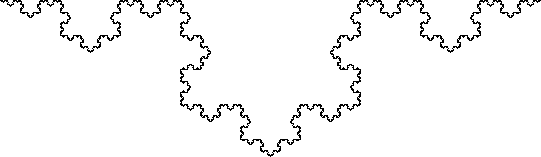
\includegraphics[width=0.9\textwidth]{koch}

    \vspace*{2cm}

    \Large\textit{\authors}

    \vspace*{\fill}

    \url{https://github.com/aelzenaar/ncea-notes}

    \makeatother
  \end{titlepage}

  \tableofcontents

  \chapter{Preamble}
  \phantomsection\addcontentsline{toc}{section}{Preface}
  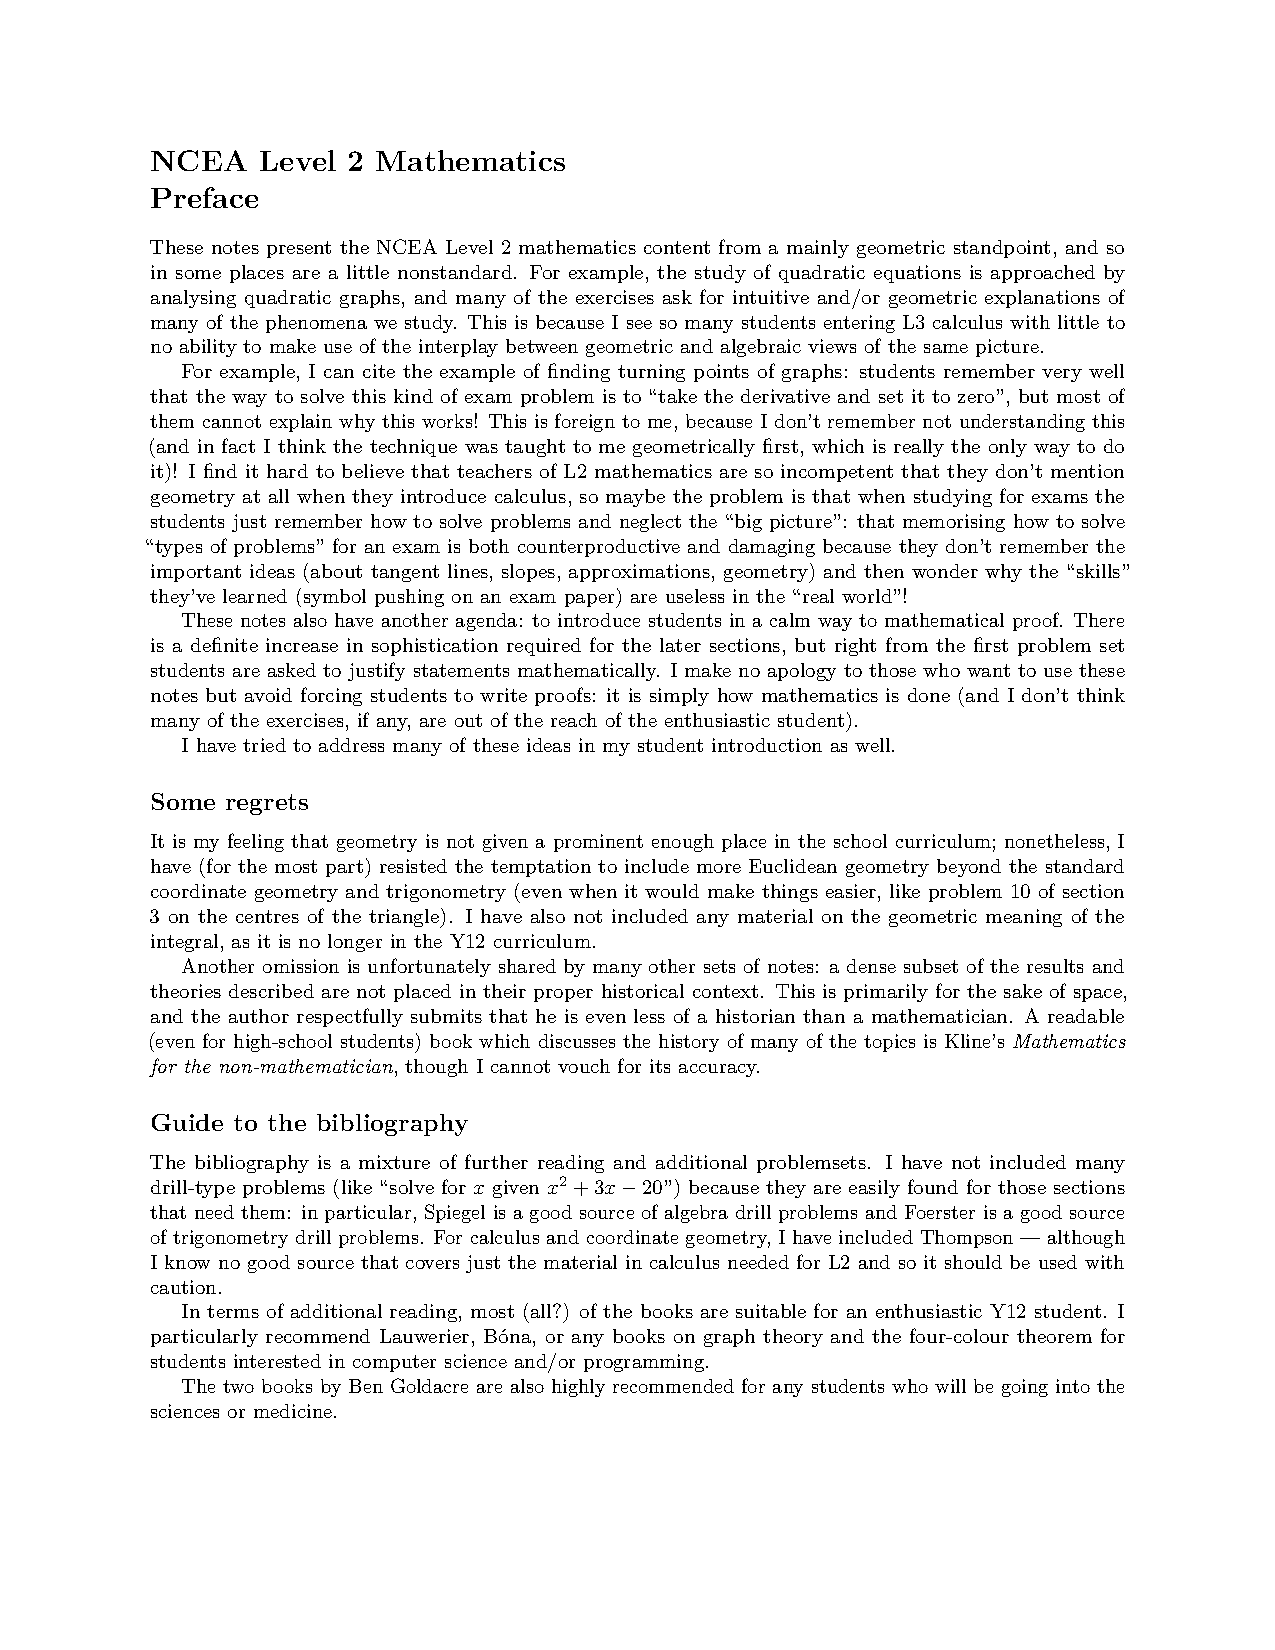
\includepdf[pages={-},pagecommand={}]{00-preface.pdf}
  \phantomsection\addcontentsline{toc}{section}{Introduction to the Notes}
  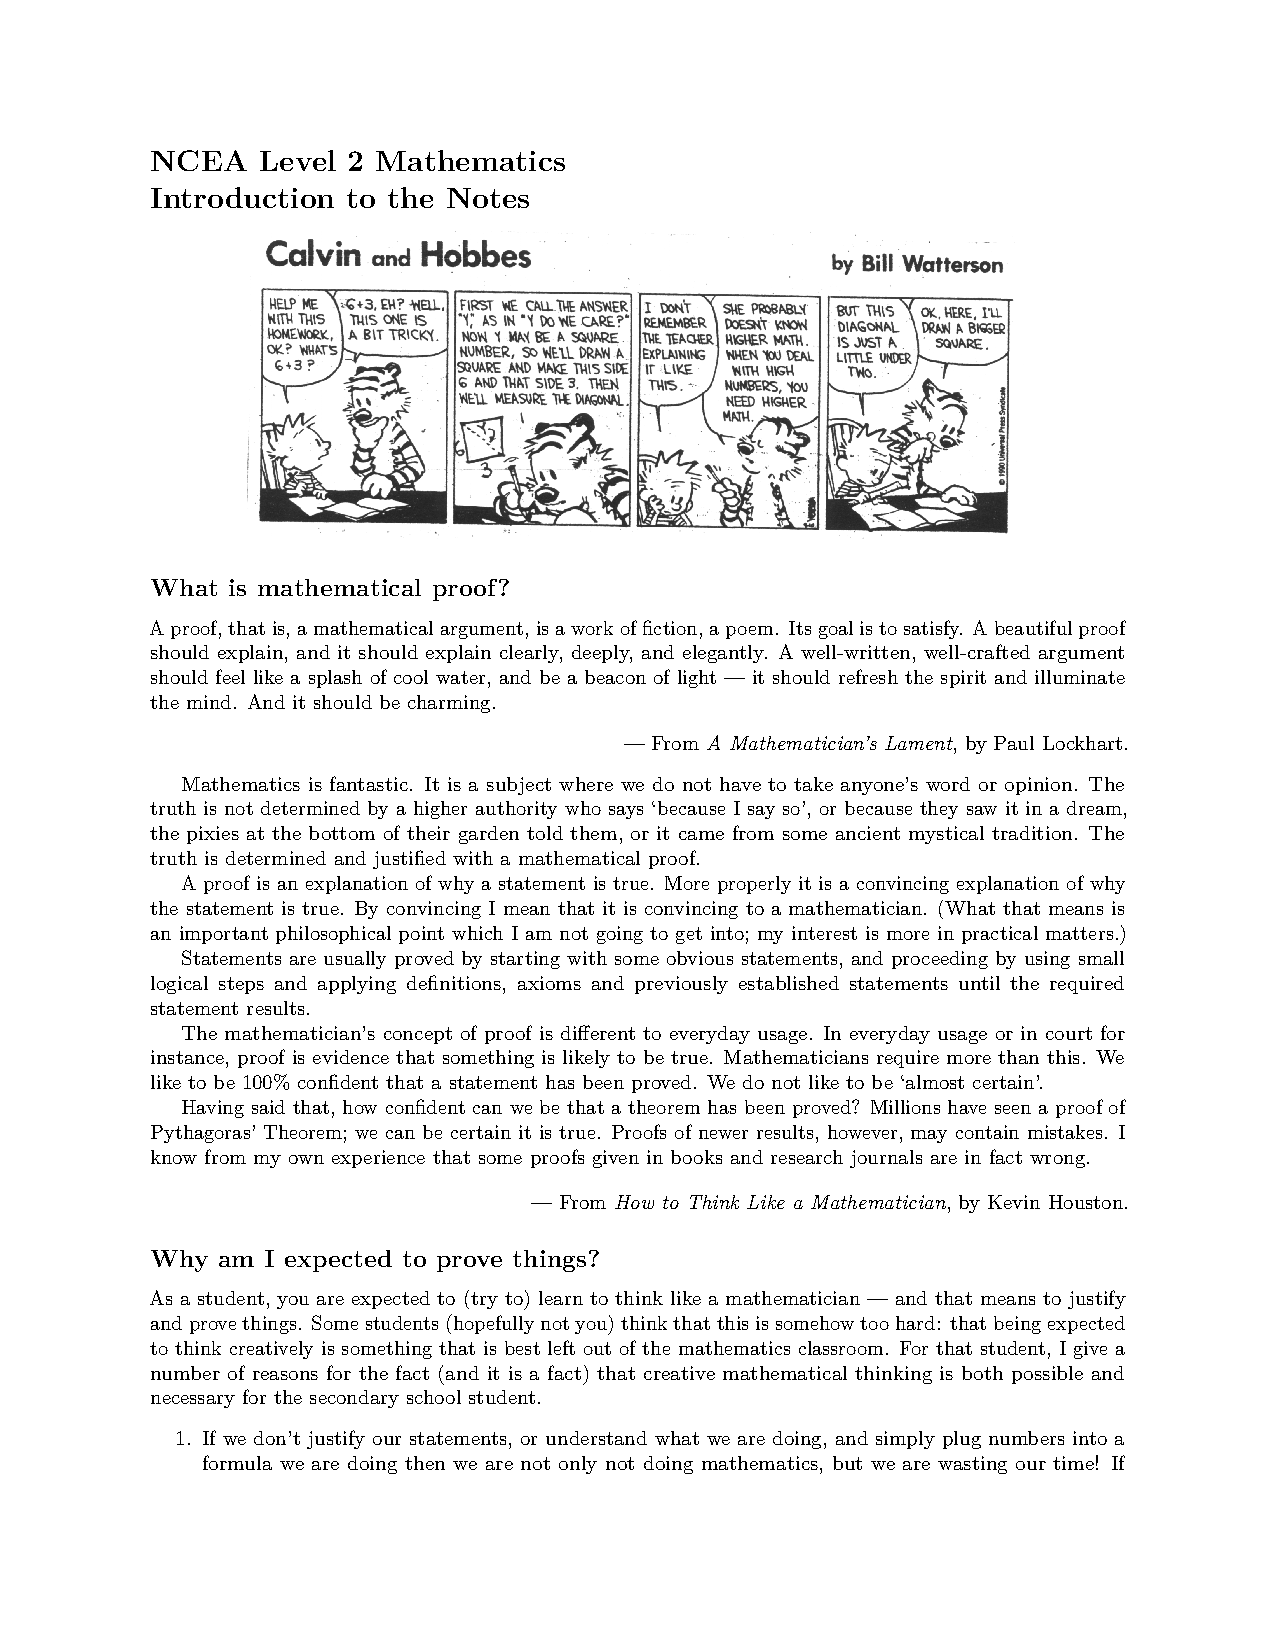
\includepdf[pages={-},pagecommand={}]{00-introduction.pdf}
  \phantomsection\addcontentsline{toc}{section}{Level 1 Revision Questions}
  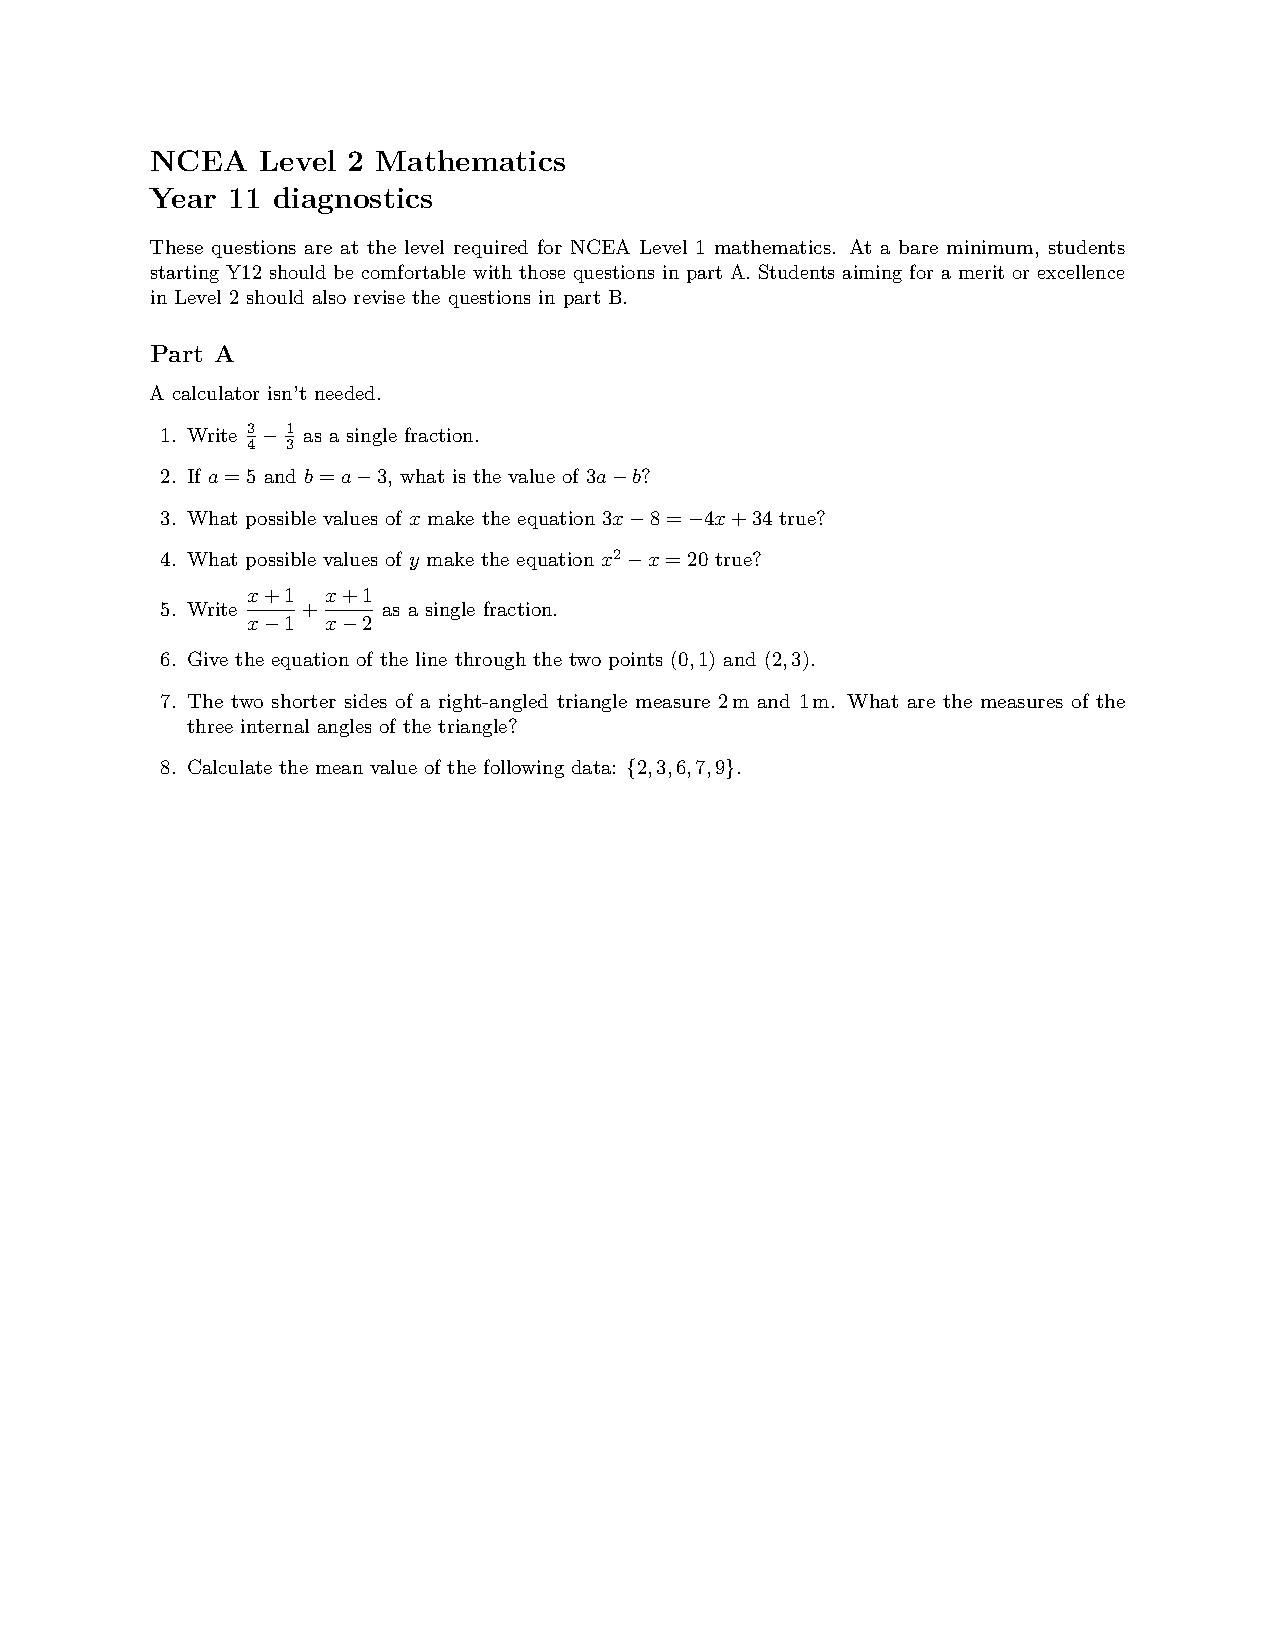
\includepdf[pages={-},pagecommand={}]{98-y11diags.pdf}

  \chapter{Geometry}
  \phantomsection\addcontentsline{toc}{section}{Coordinate Geometry}
  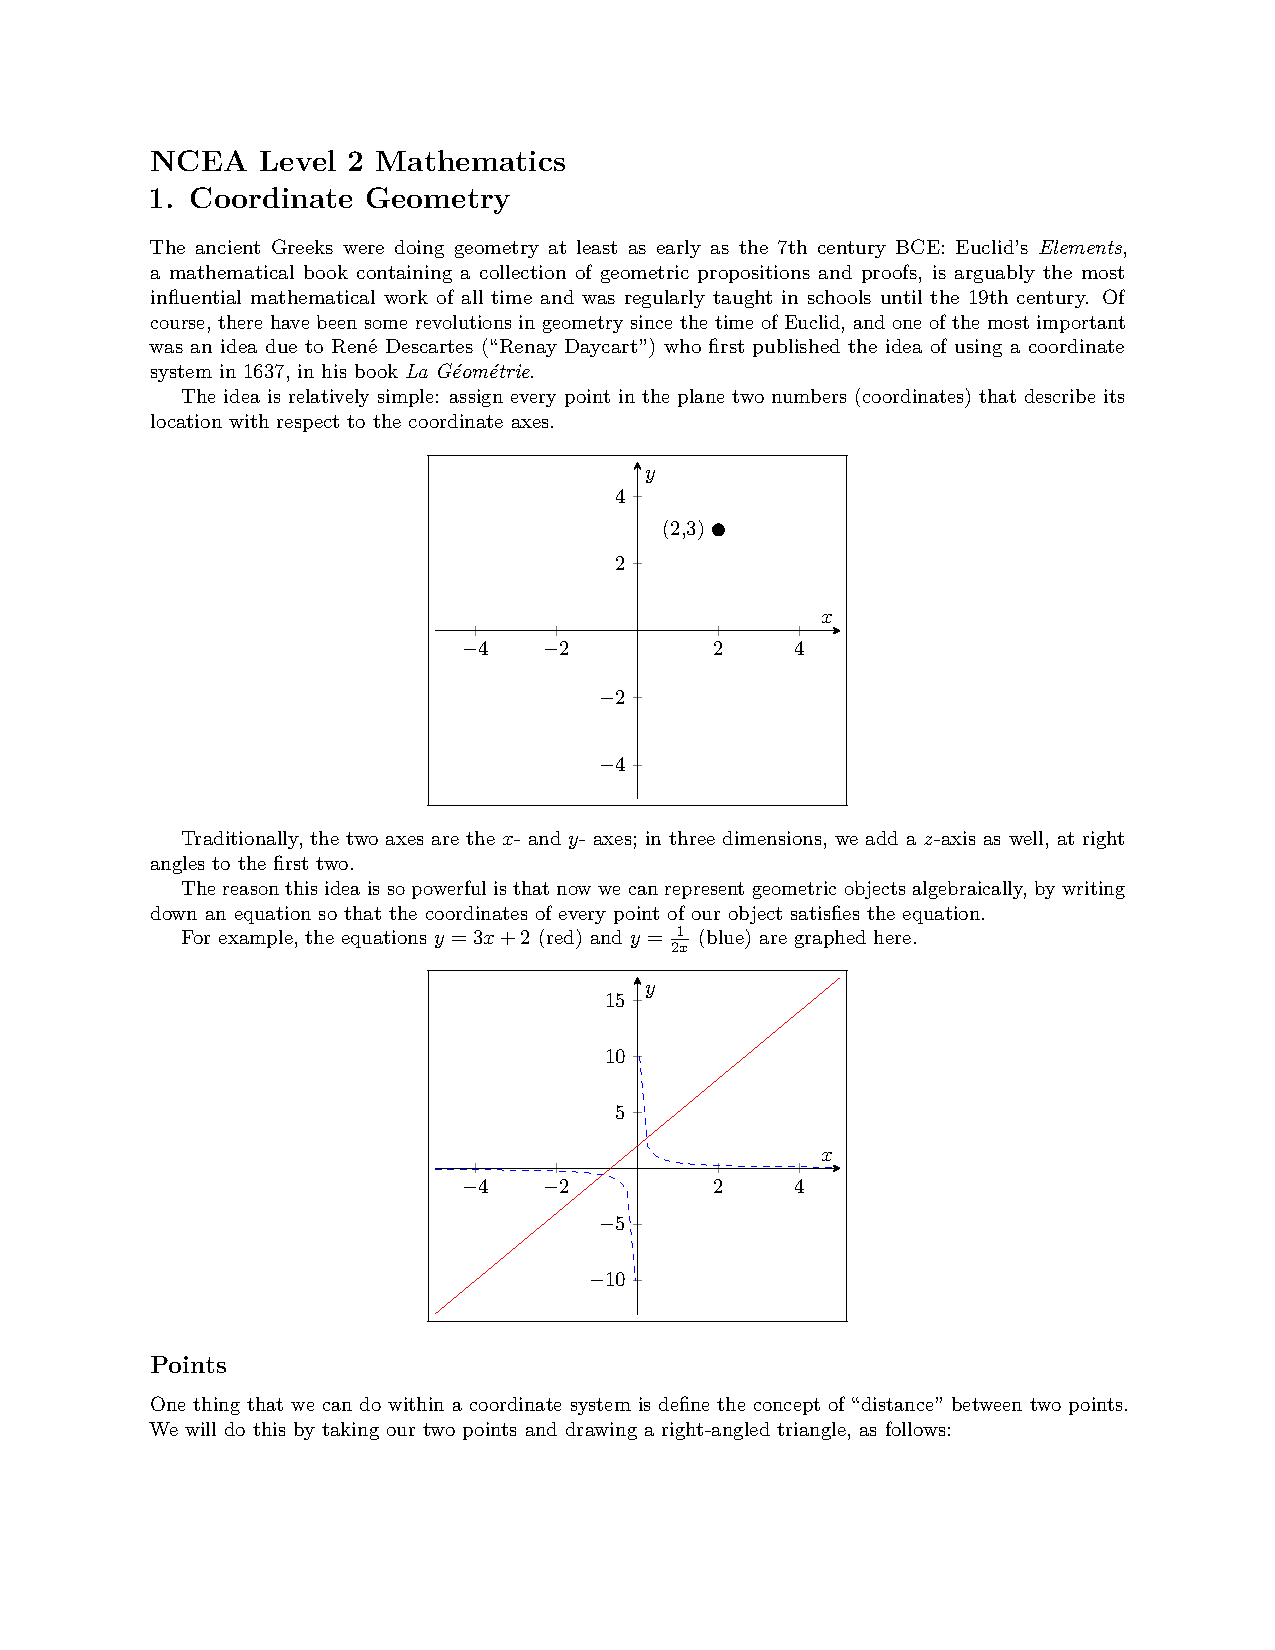
\includepdf[pages={-},pagecommand={}]{01-coordgeom.pdf}
  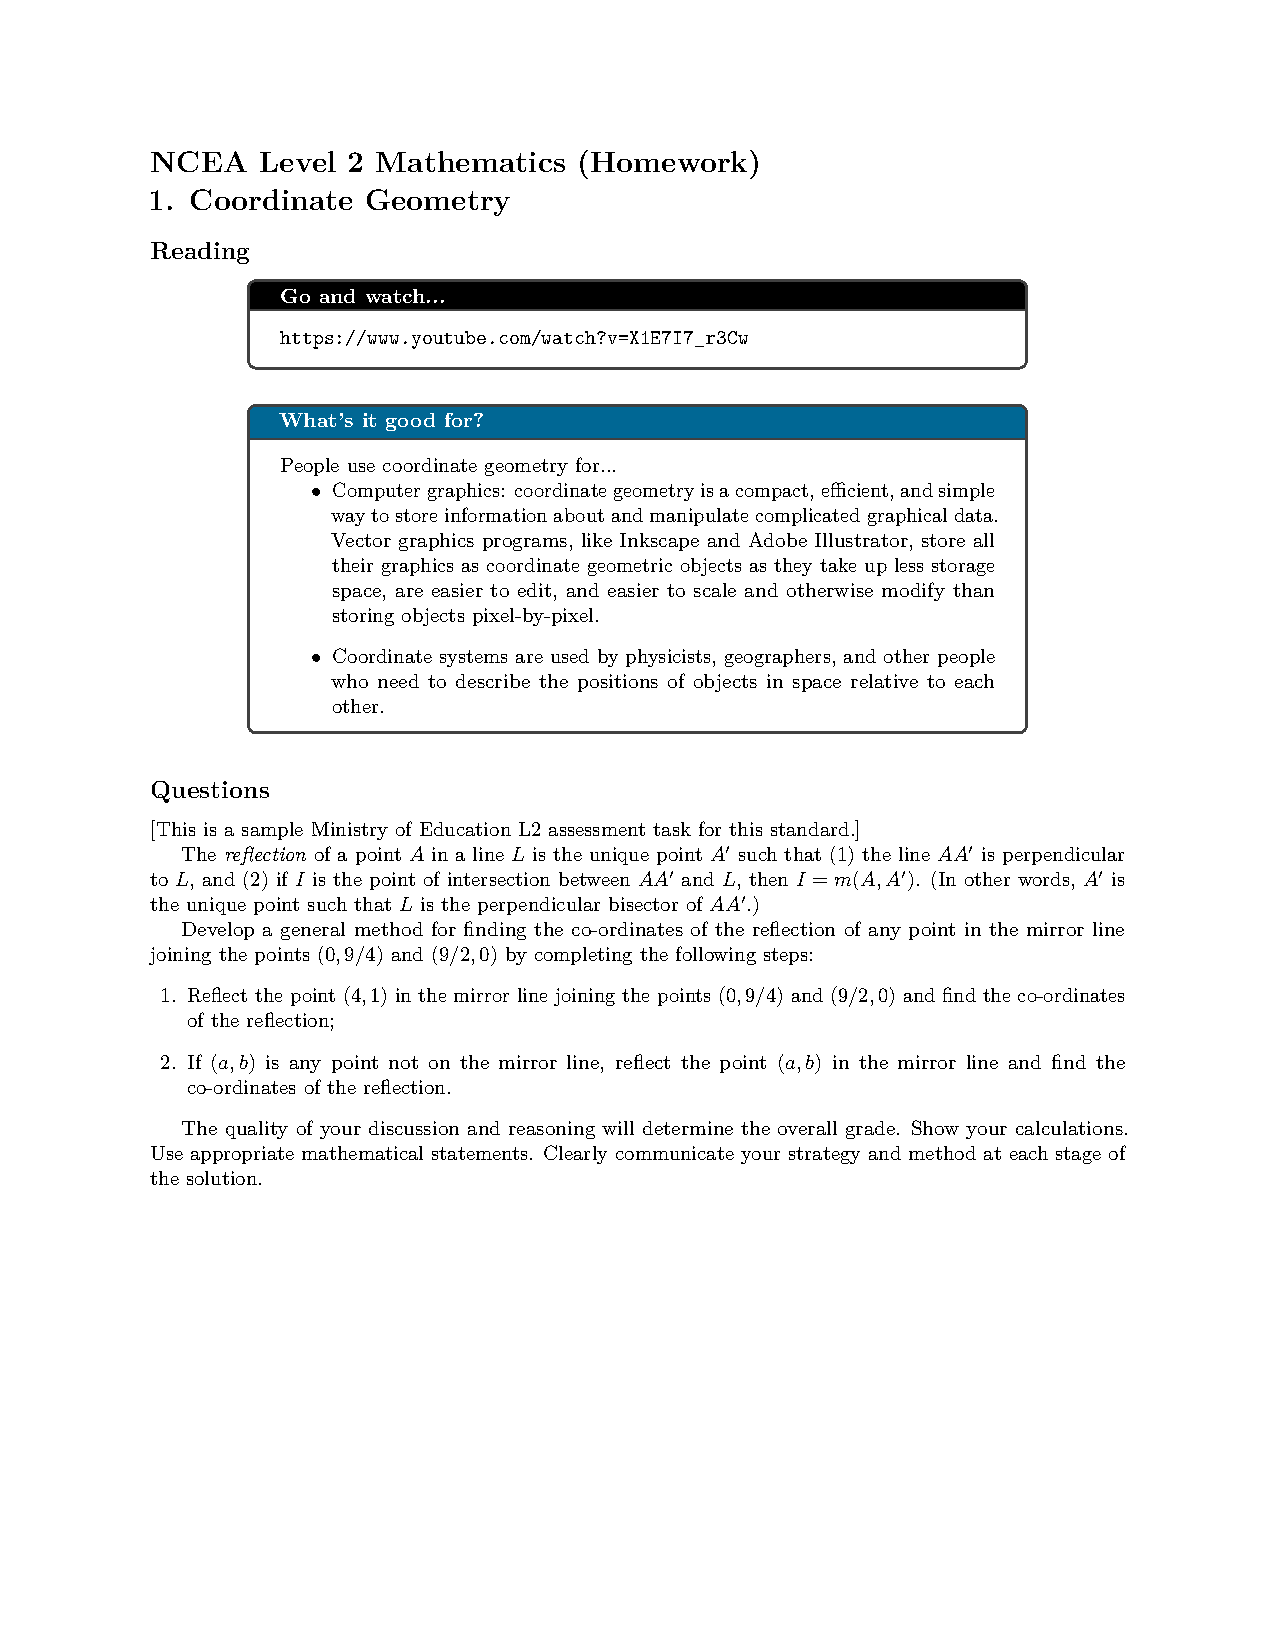
\includepdf[pages={-},pagecommand={}]{01-coordgeom-hw.pdf}
  \phantomsection\addcontentsline{toc}{section}{Arcs and Sectors of Circles}
  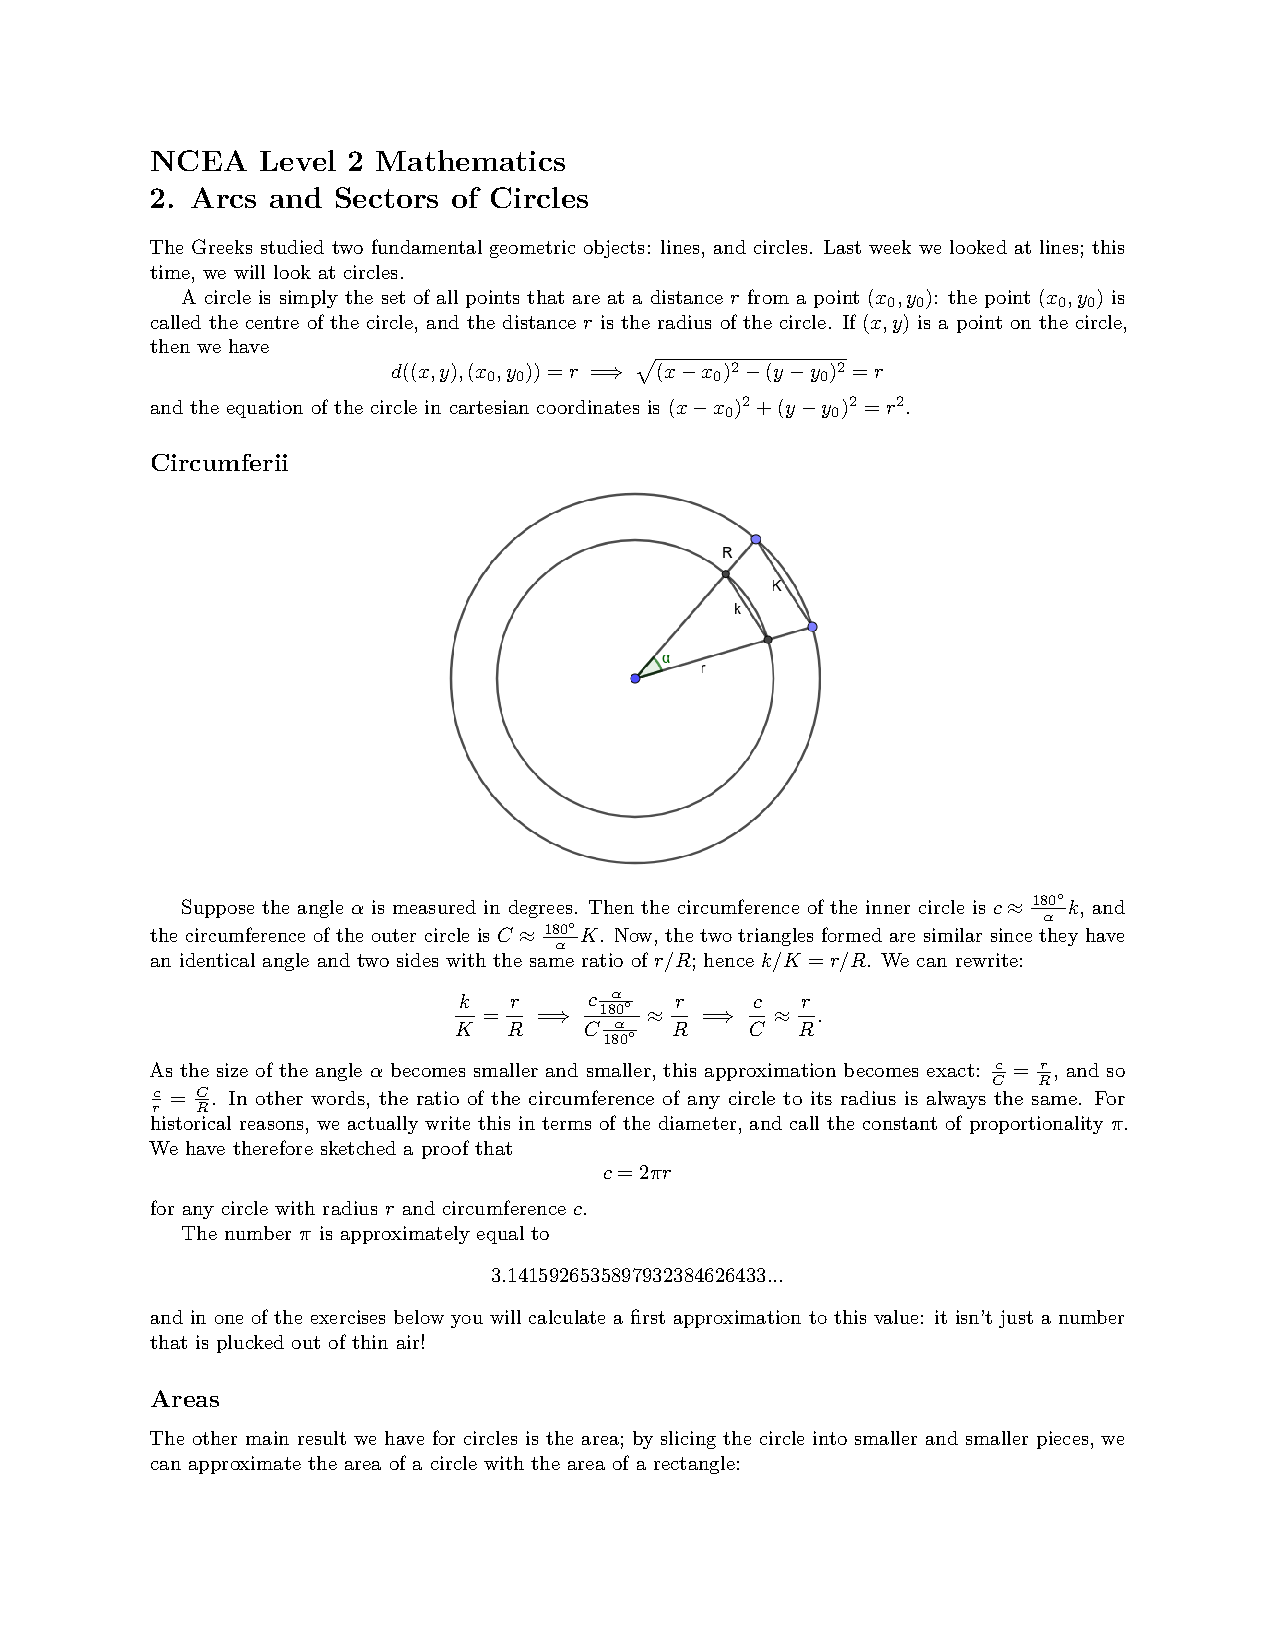
\includepdf[pages={-},pagecommand={}]{02-circles.pdf}
  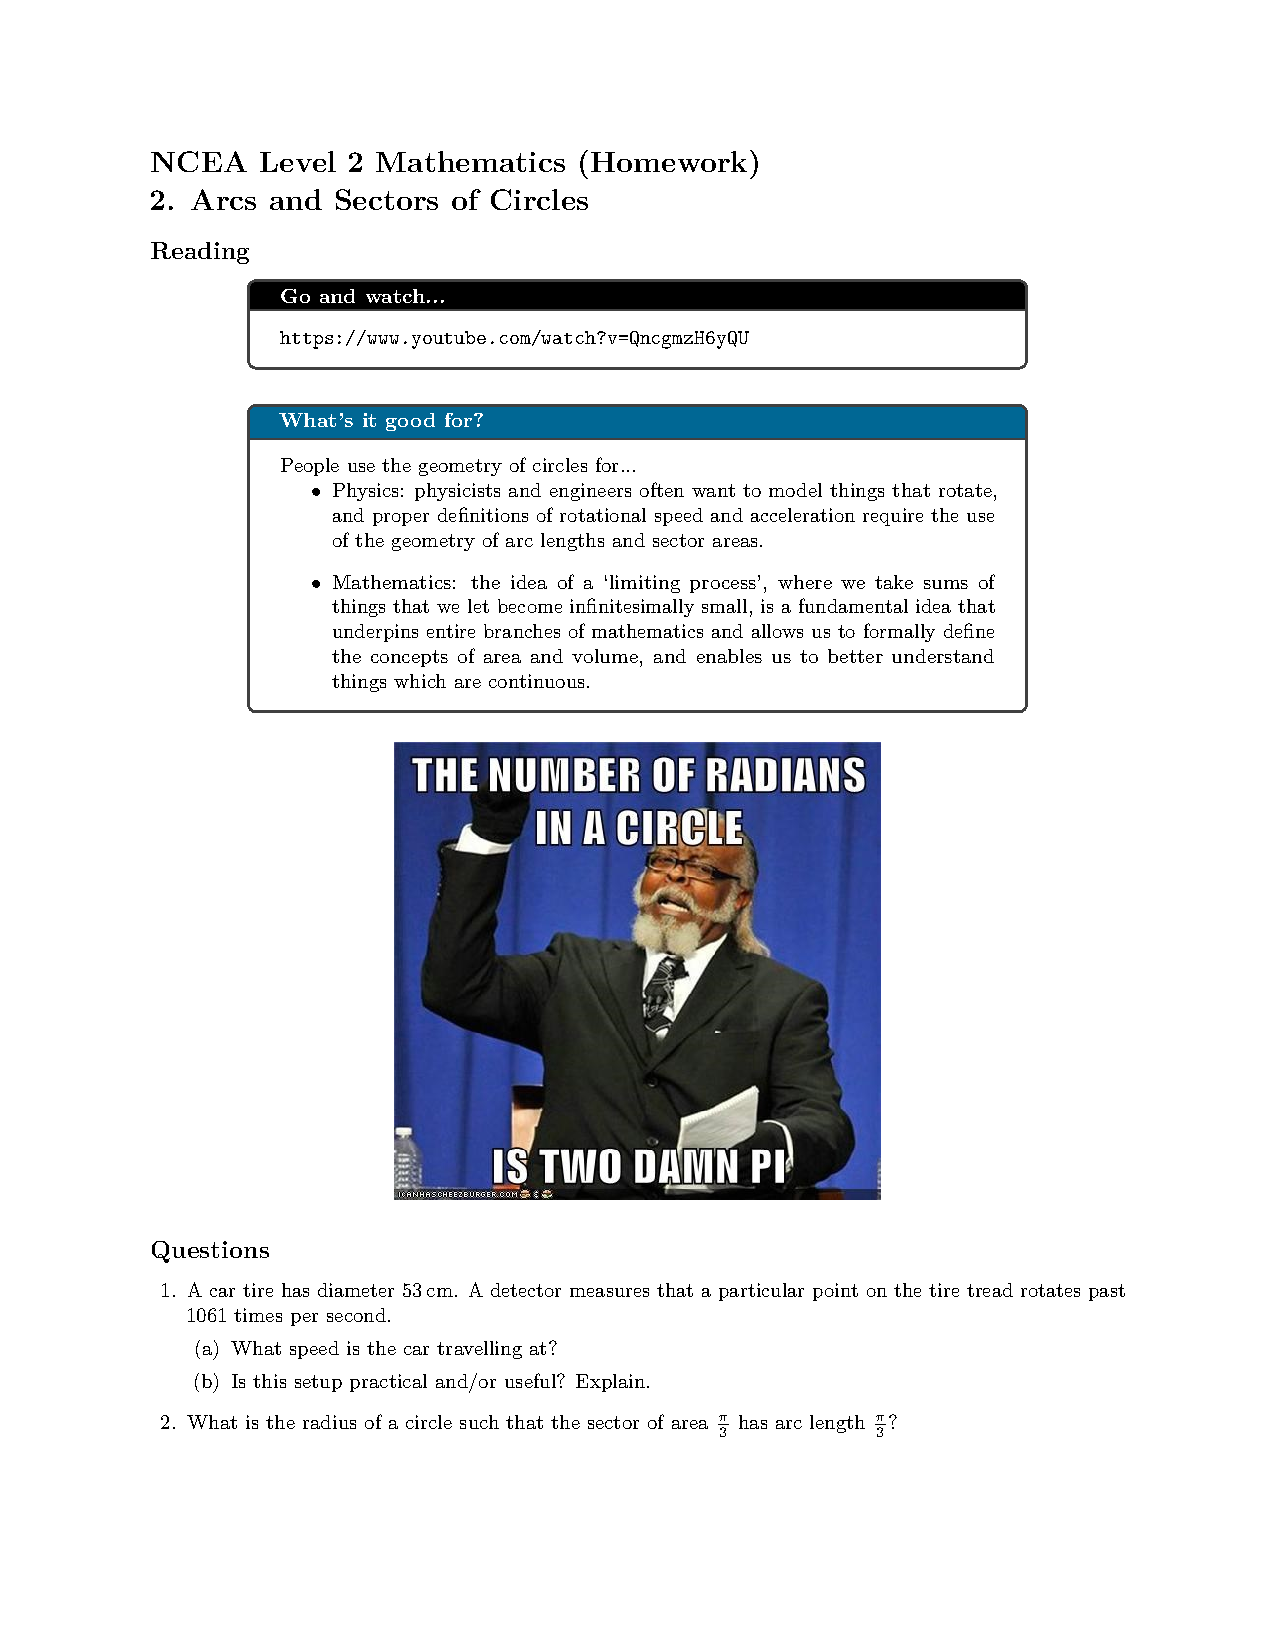
\includepdf[pages={-},pagecommand={}]{02-circles-hw.pdf}
  \phantomsection\addcontentsline{toc}{section}{Trigonometry}
  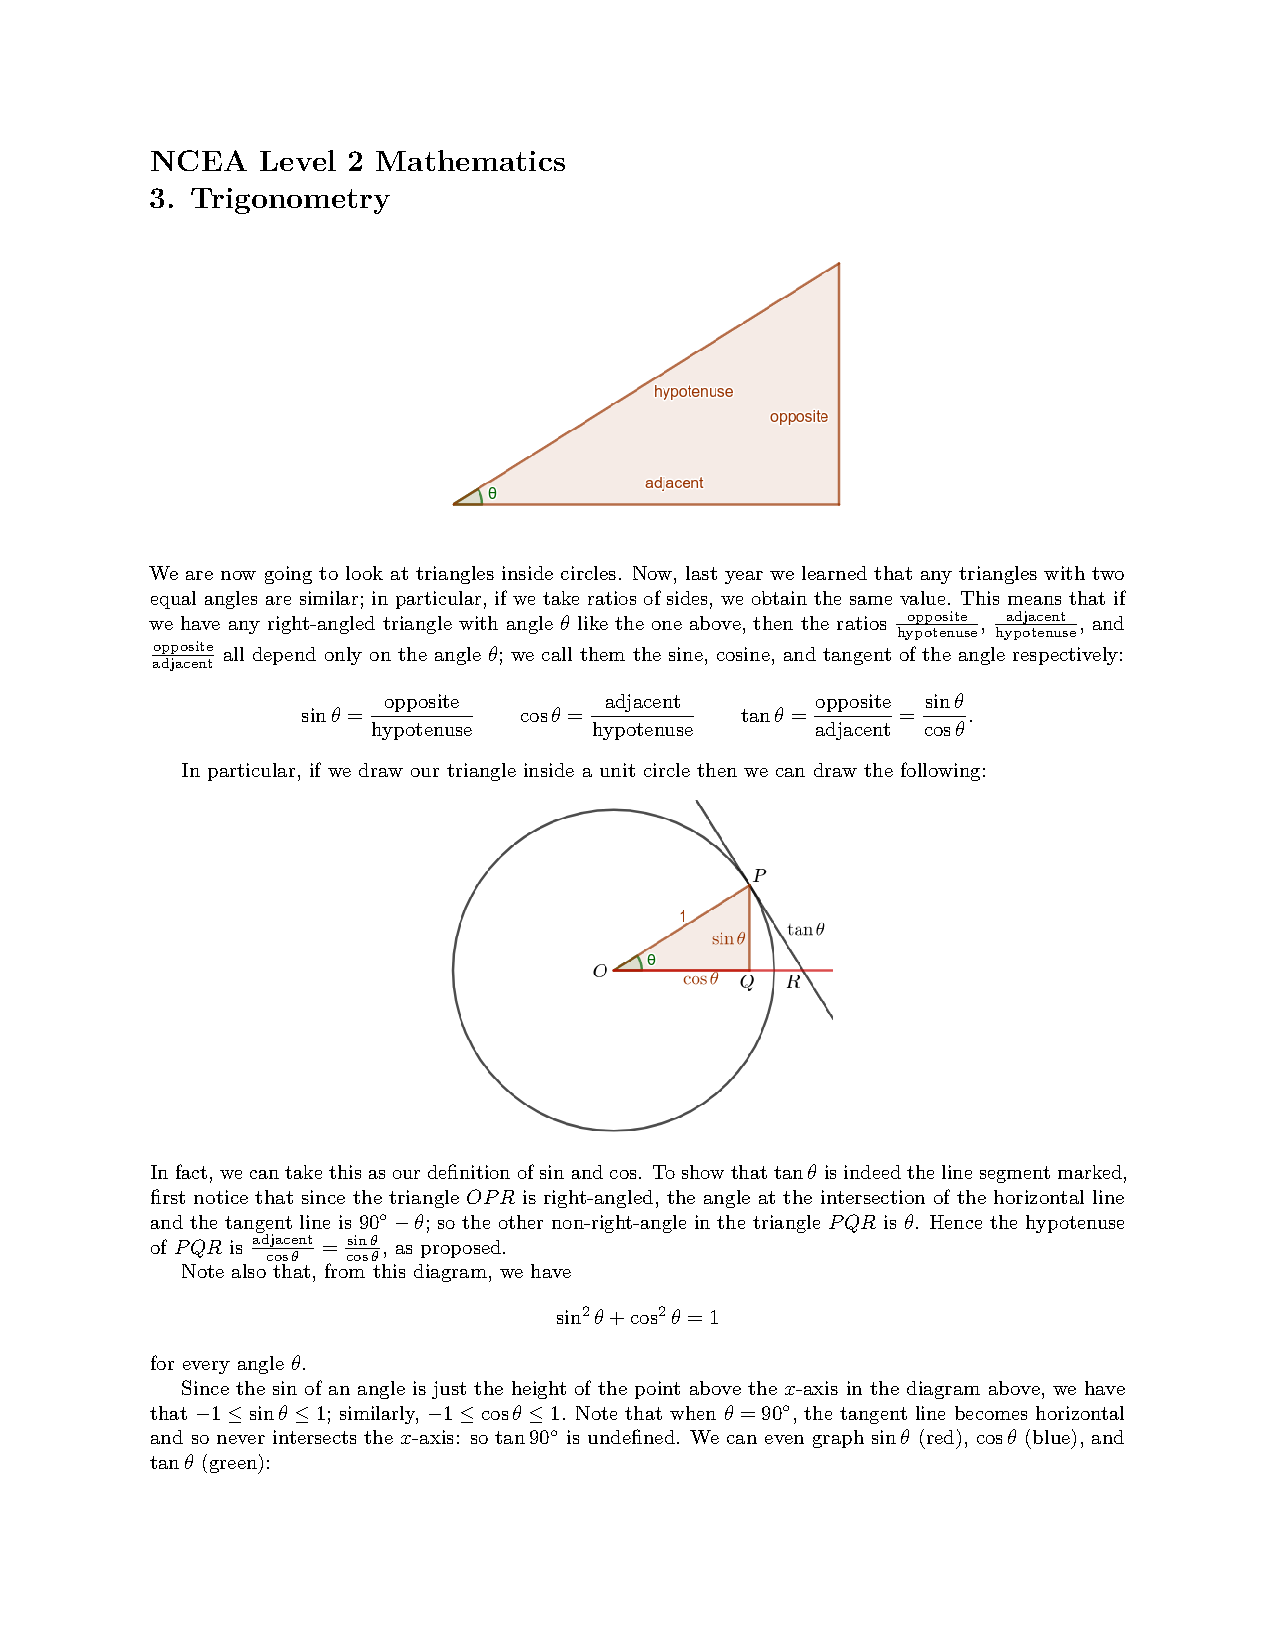
\includepdf[pages={-},pagecommand={}]{03-trig.pdf}
  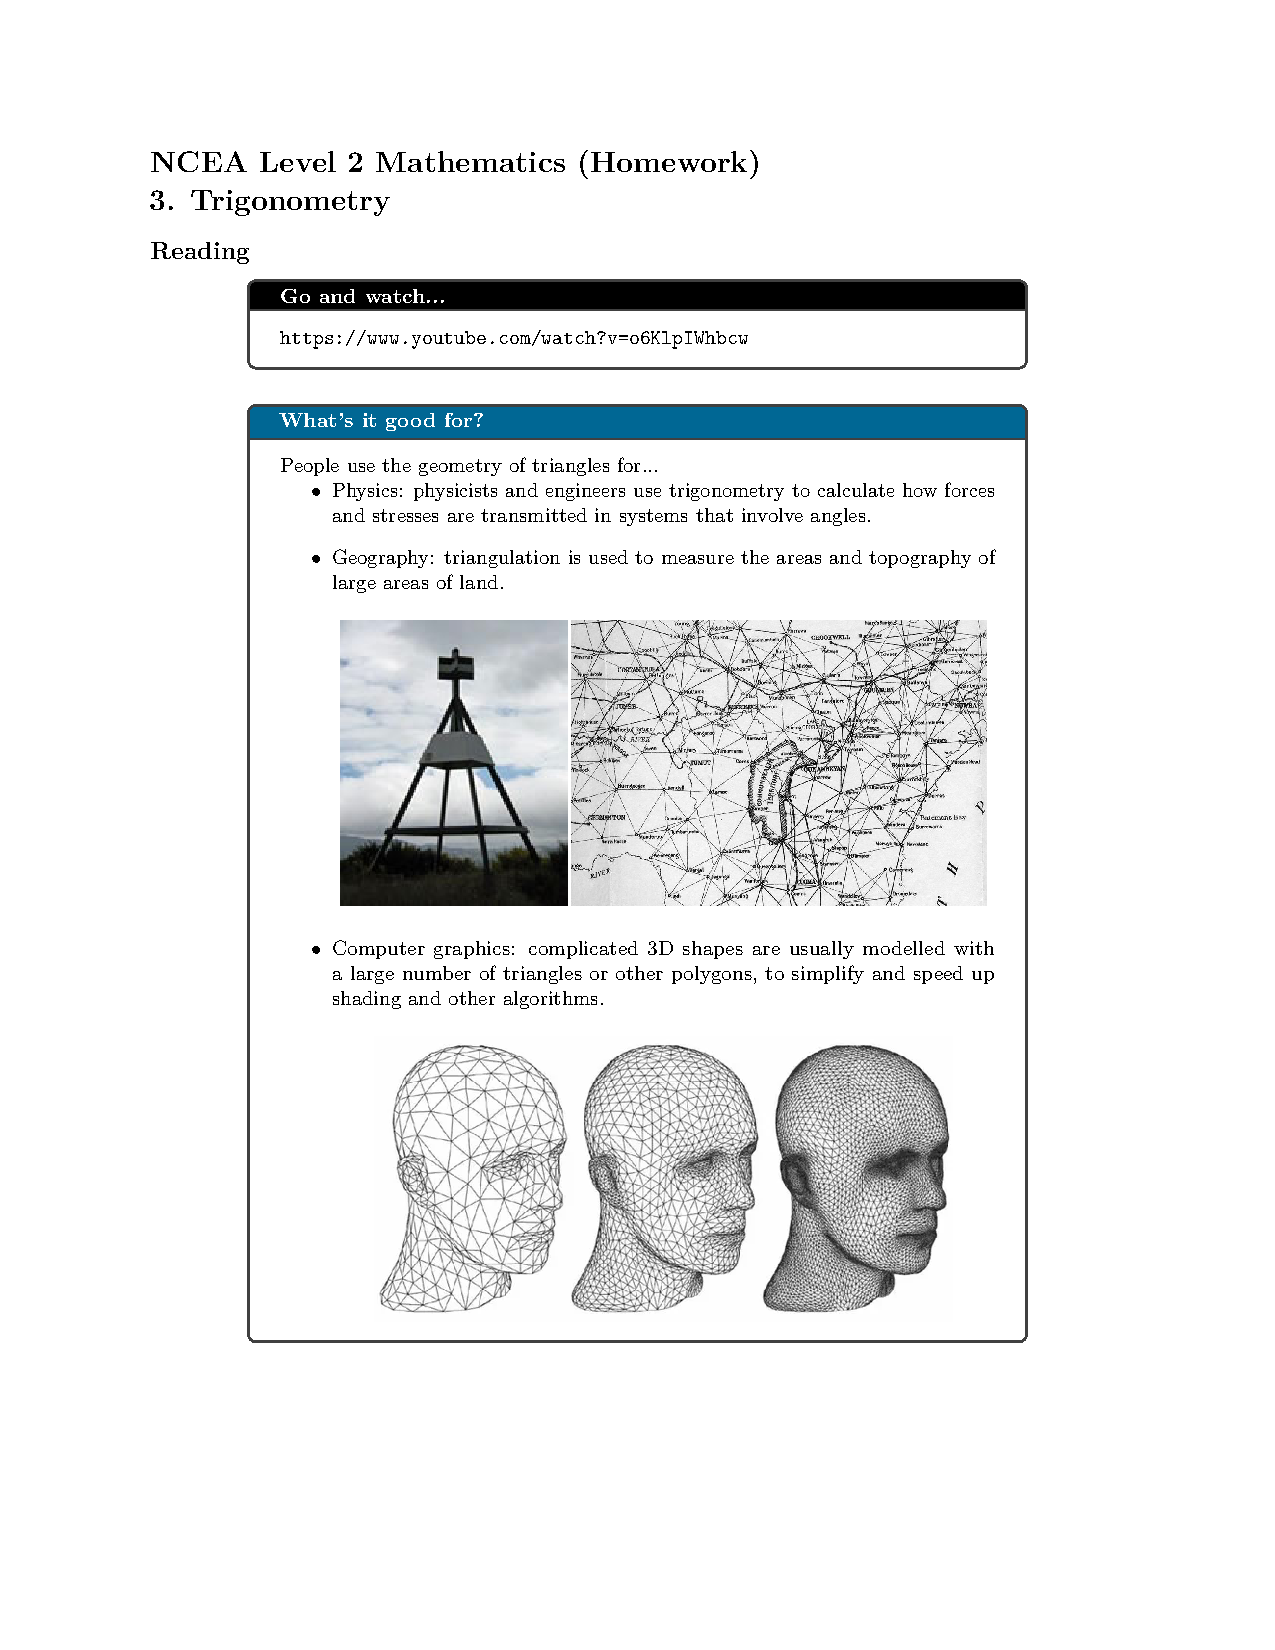
\includepdf[pages={-},pagecommand={}]{03-trig-hw.pdf}

  \chapter{Algebra}
  \phantomsection\addcontentsline{toc}{section}{Functions}
  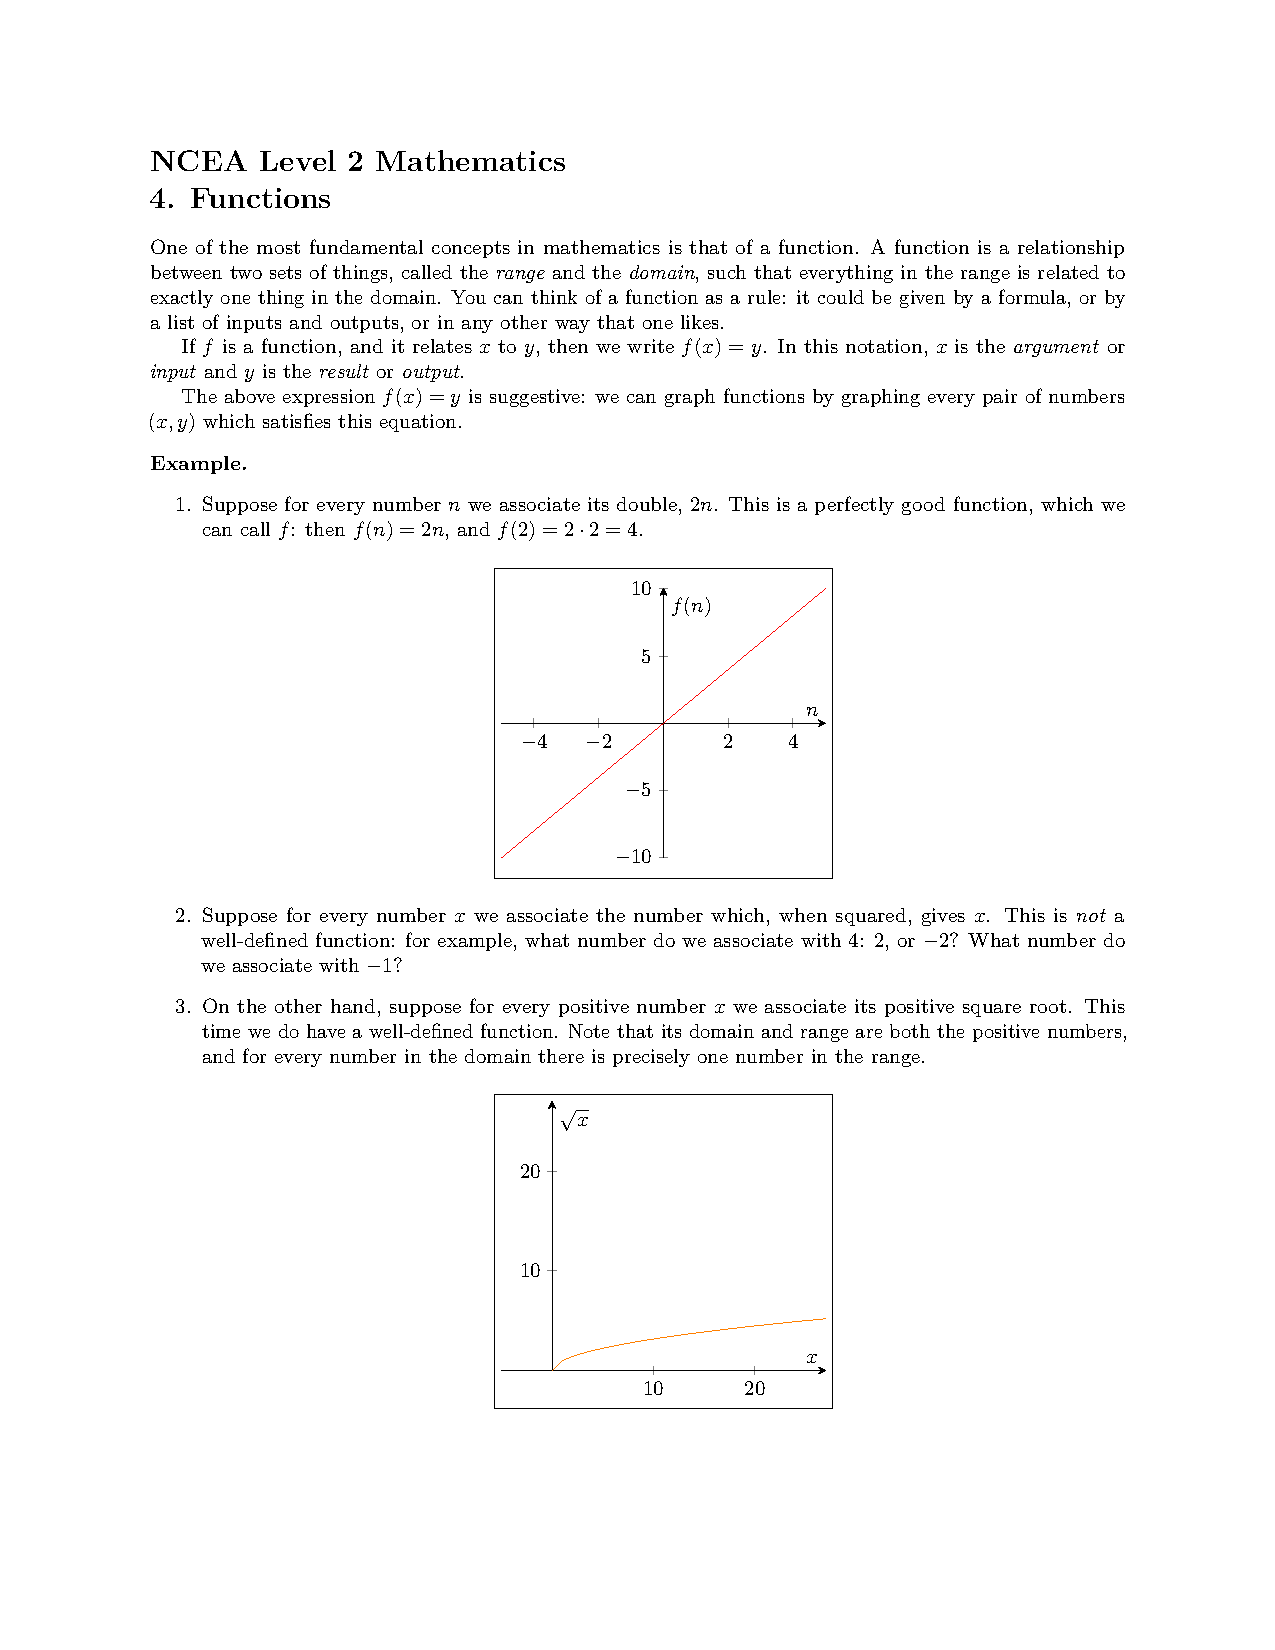
\includepdf[pages={-},pagecommand={}]{04-functions.pdf}
  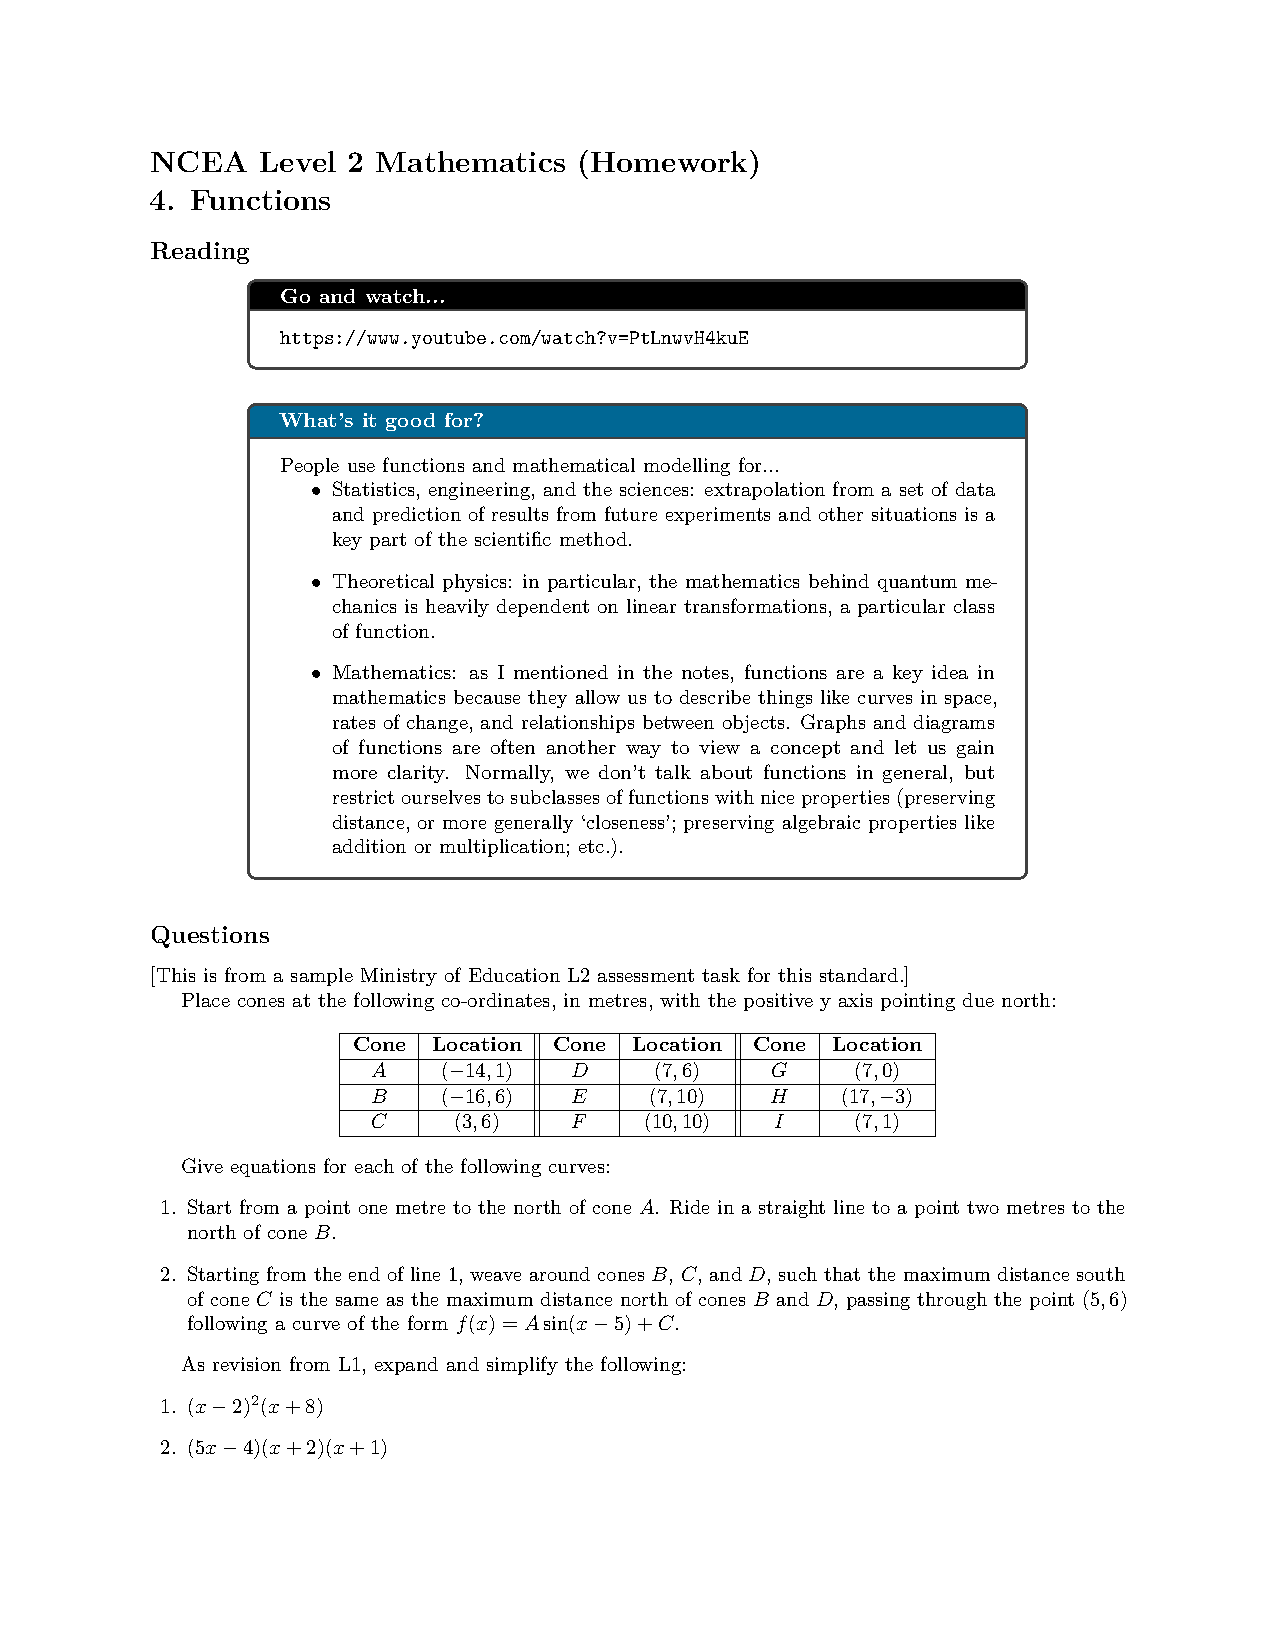
\includepdf[pages={-},pagecommand={}]{04-functions-hw.pdf}
  \phantomsection\addcontentsline{toc}{section}{Quadratic Modelling}
  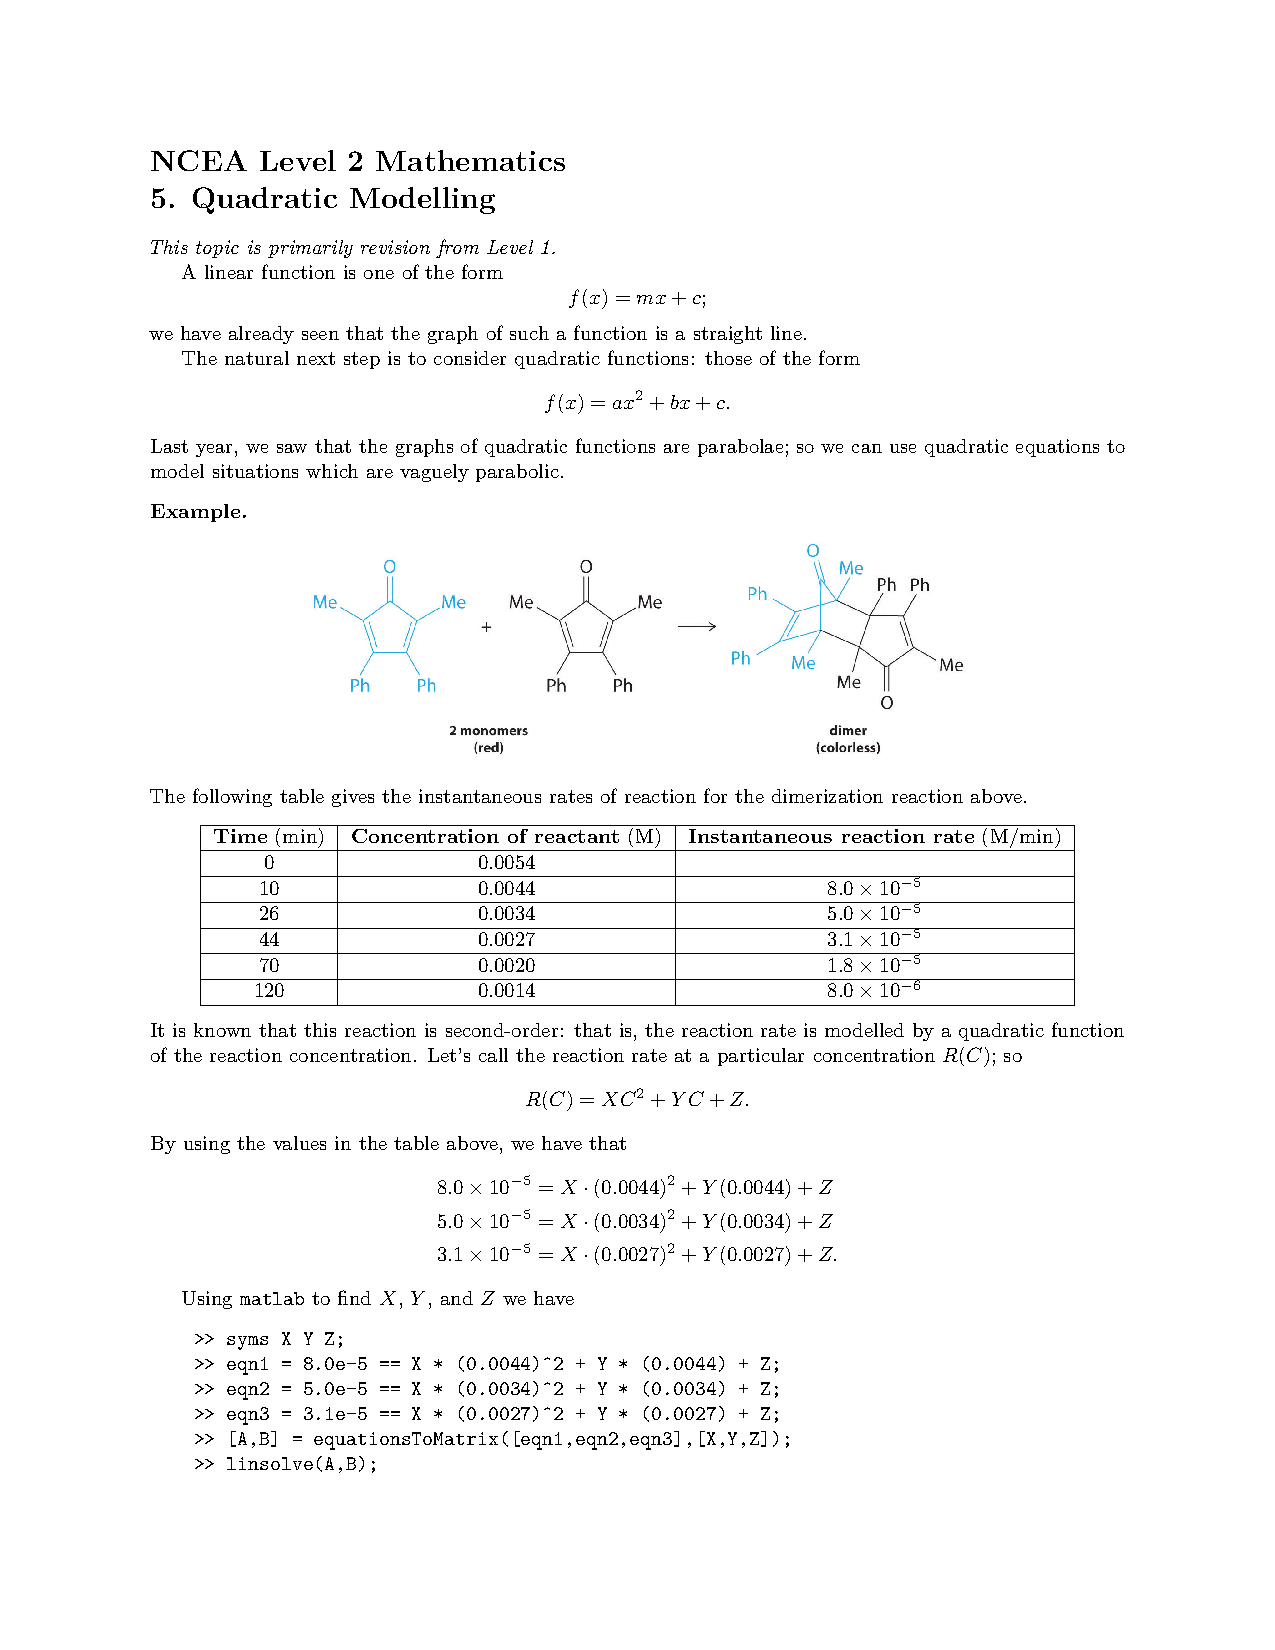
\includepdf[pages={-},pagecommand={}]{05-quadratics.pdf}
  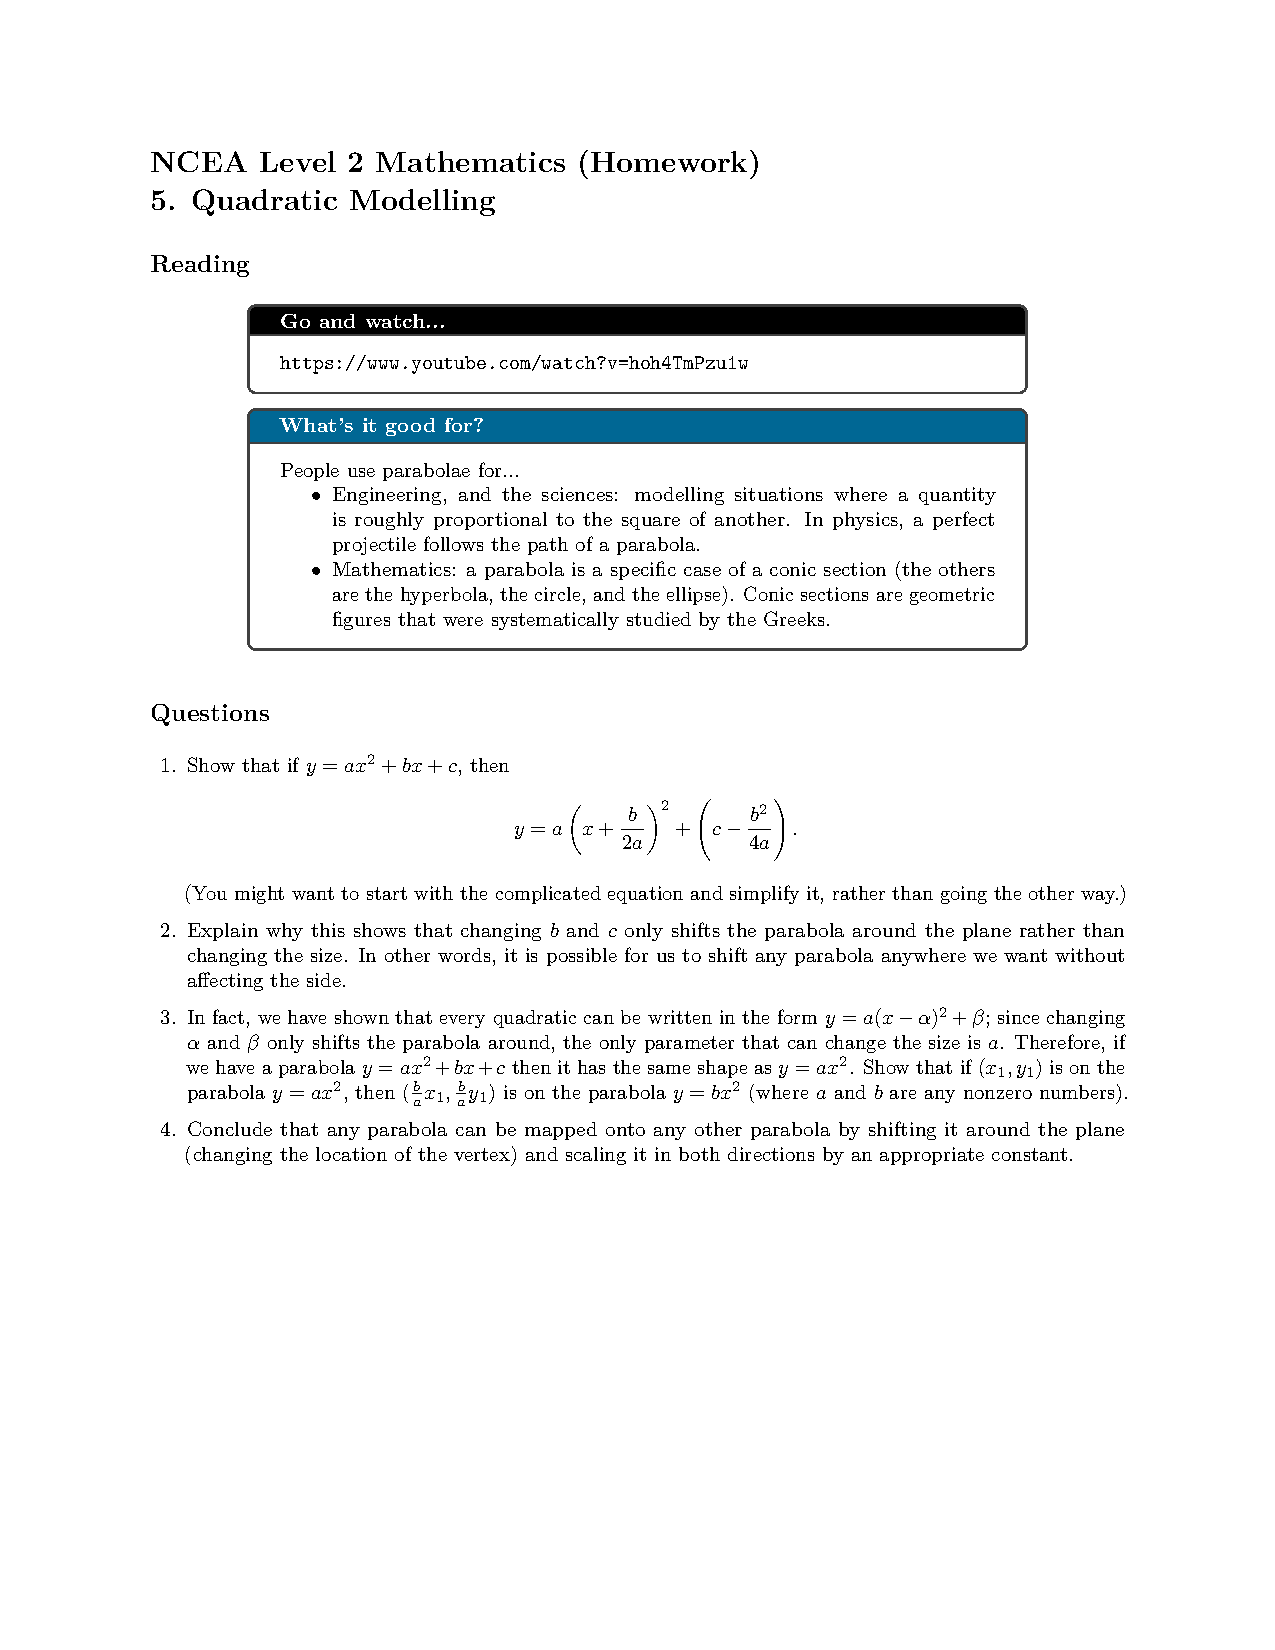
\includepdf[pages={-},pagecommand={}]{05-quadratics-hw.pdf}
  \phantomsection\addcontentsline{toc}{section}{Simultaneous Equations}
  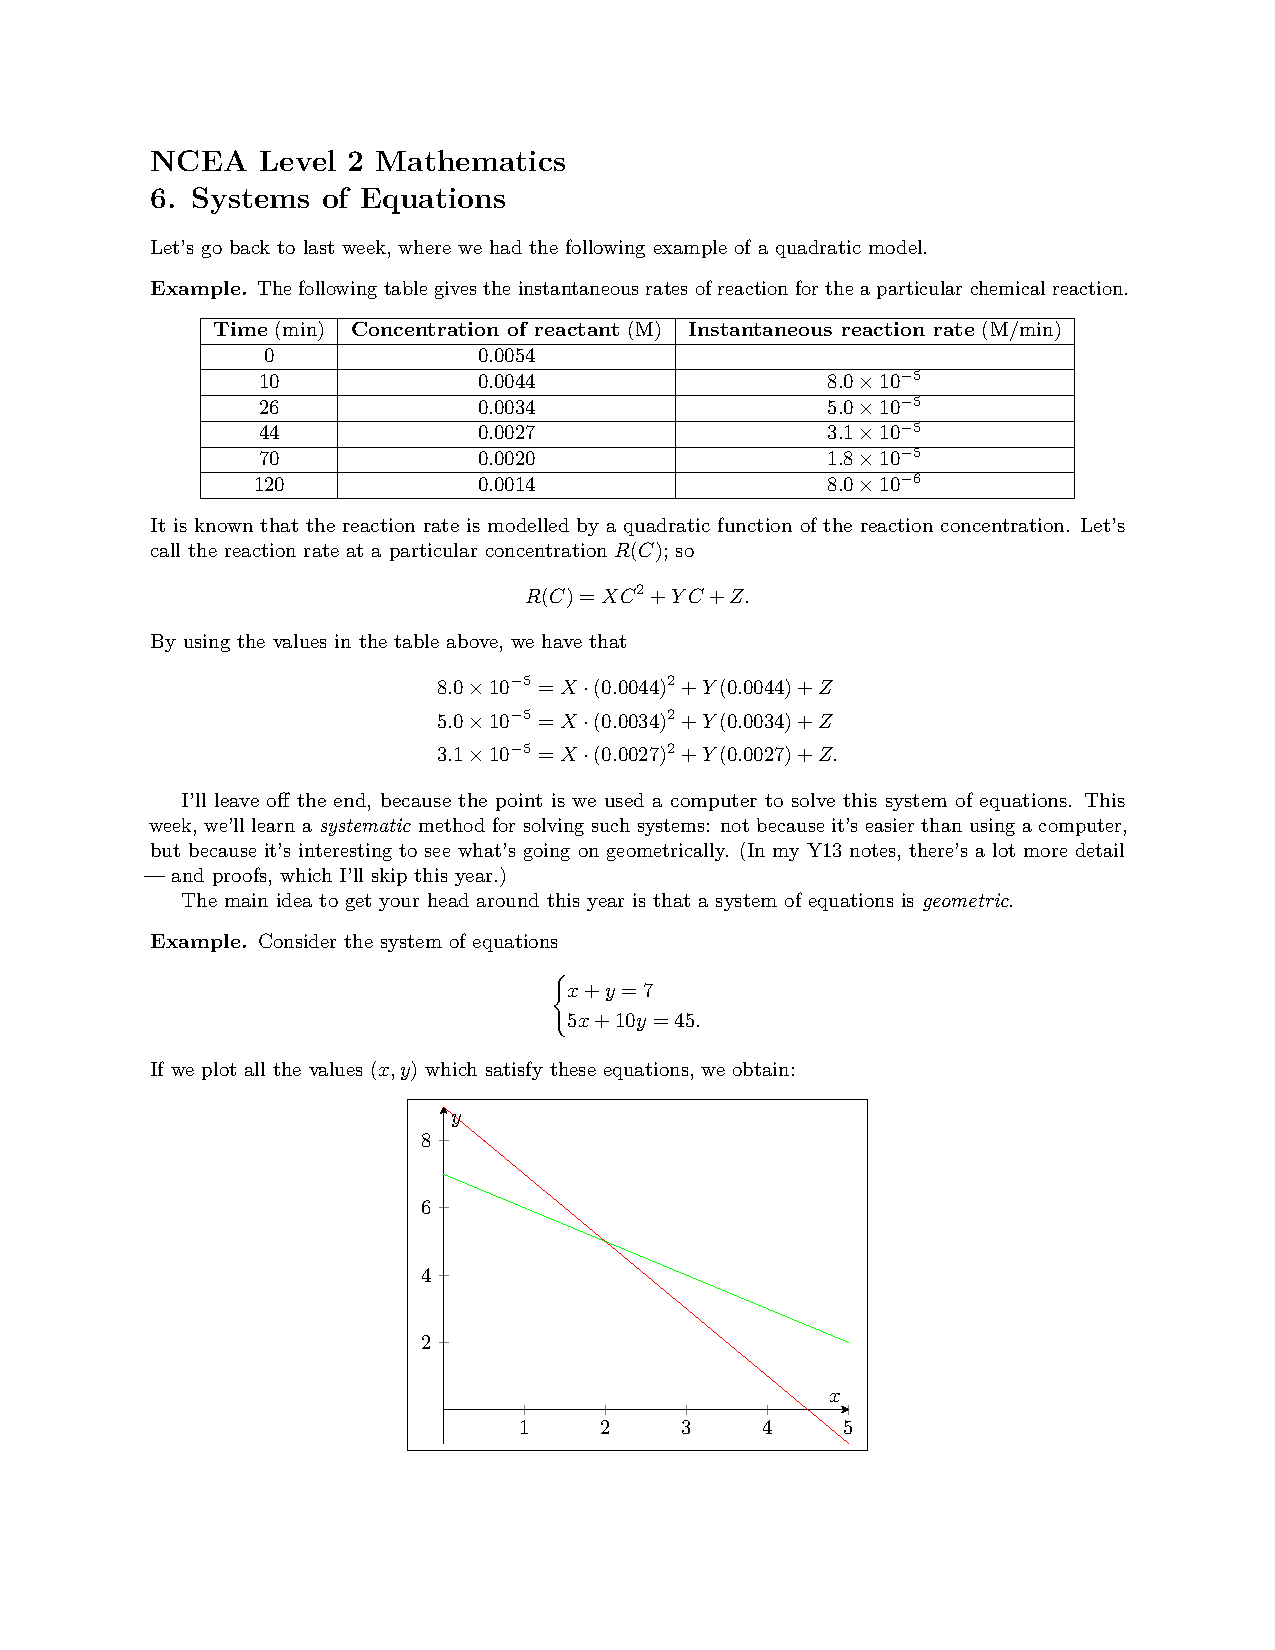
\includepdf[pages={-},pagecommand={}]{06-simeqs.pdf}
  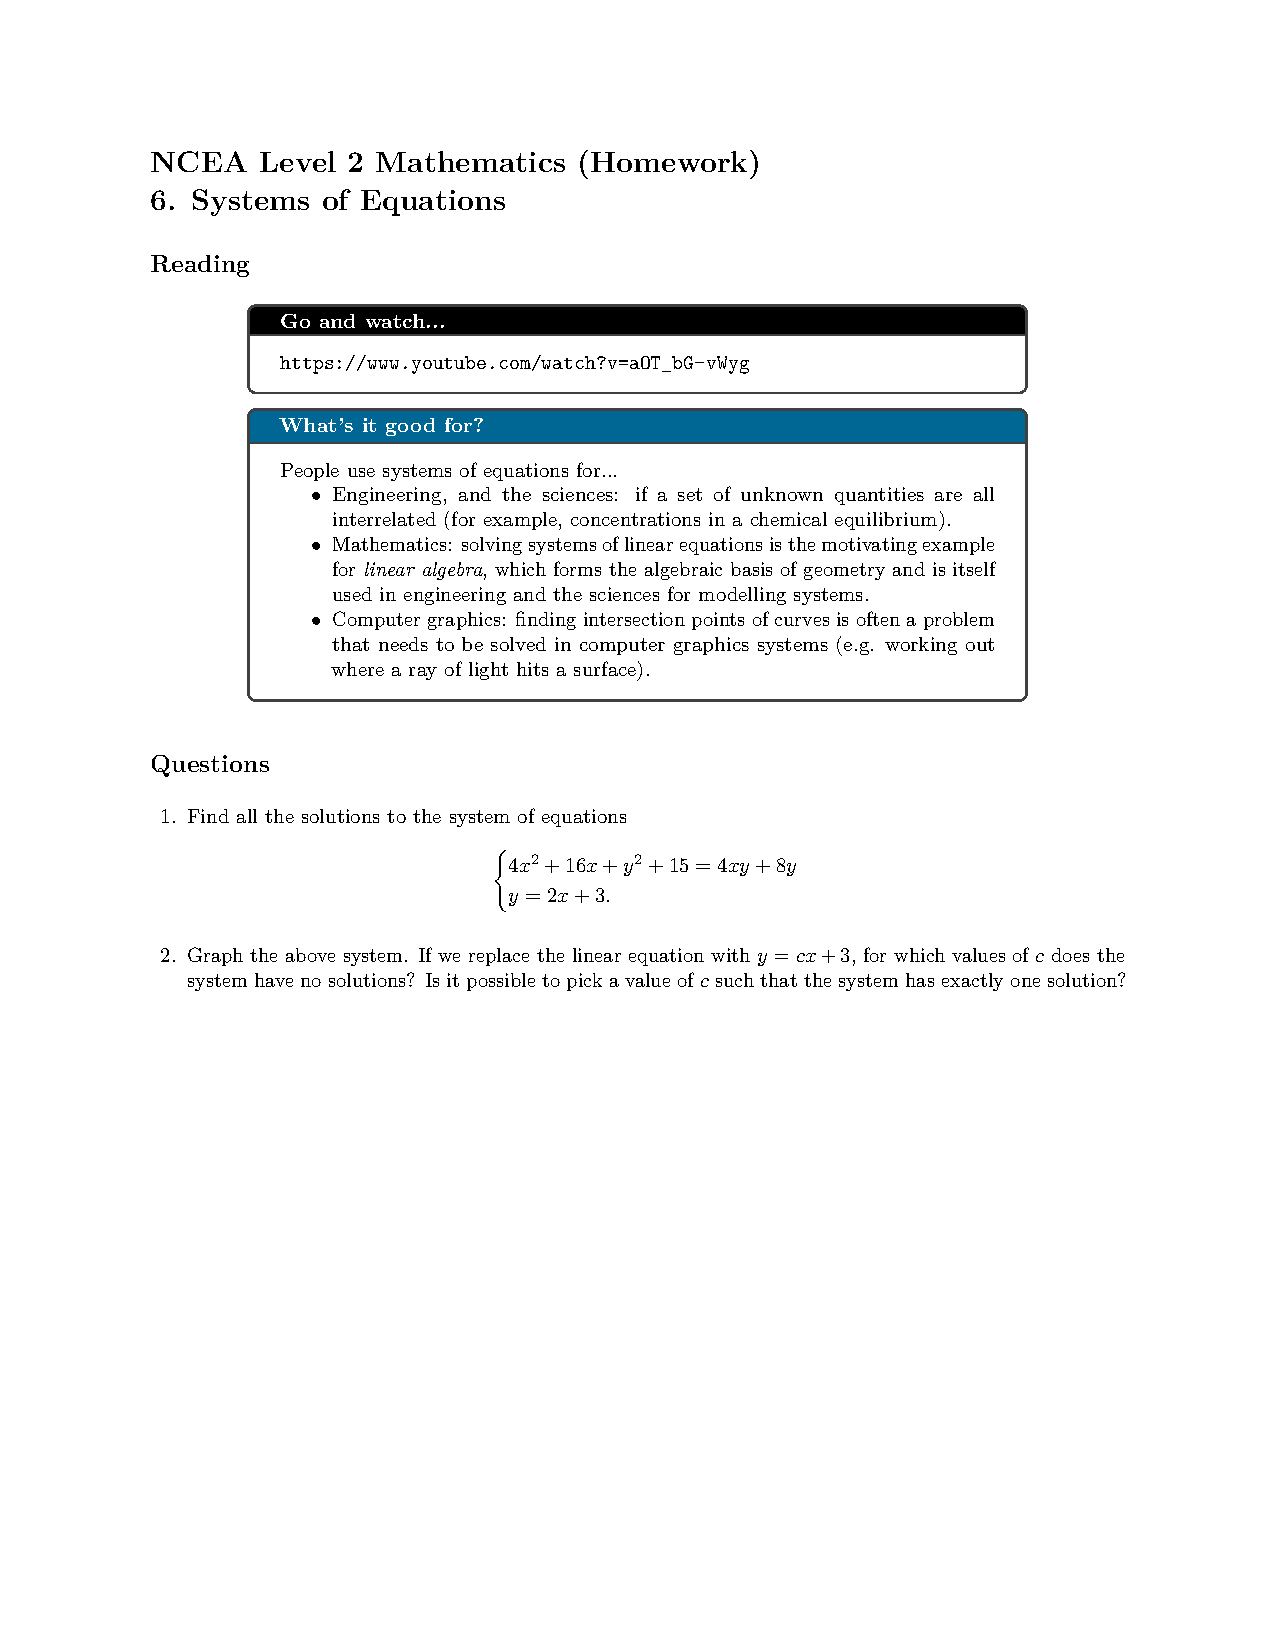
\includepdf[pages={-},pagecommand={}]{06-simeqs-hw.pdf}
  \phantomsection\addcontentsline{toc}{section}{Linear Inequalities}
  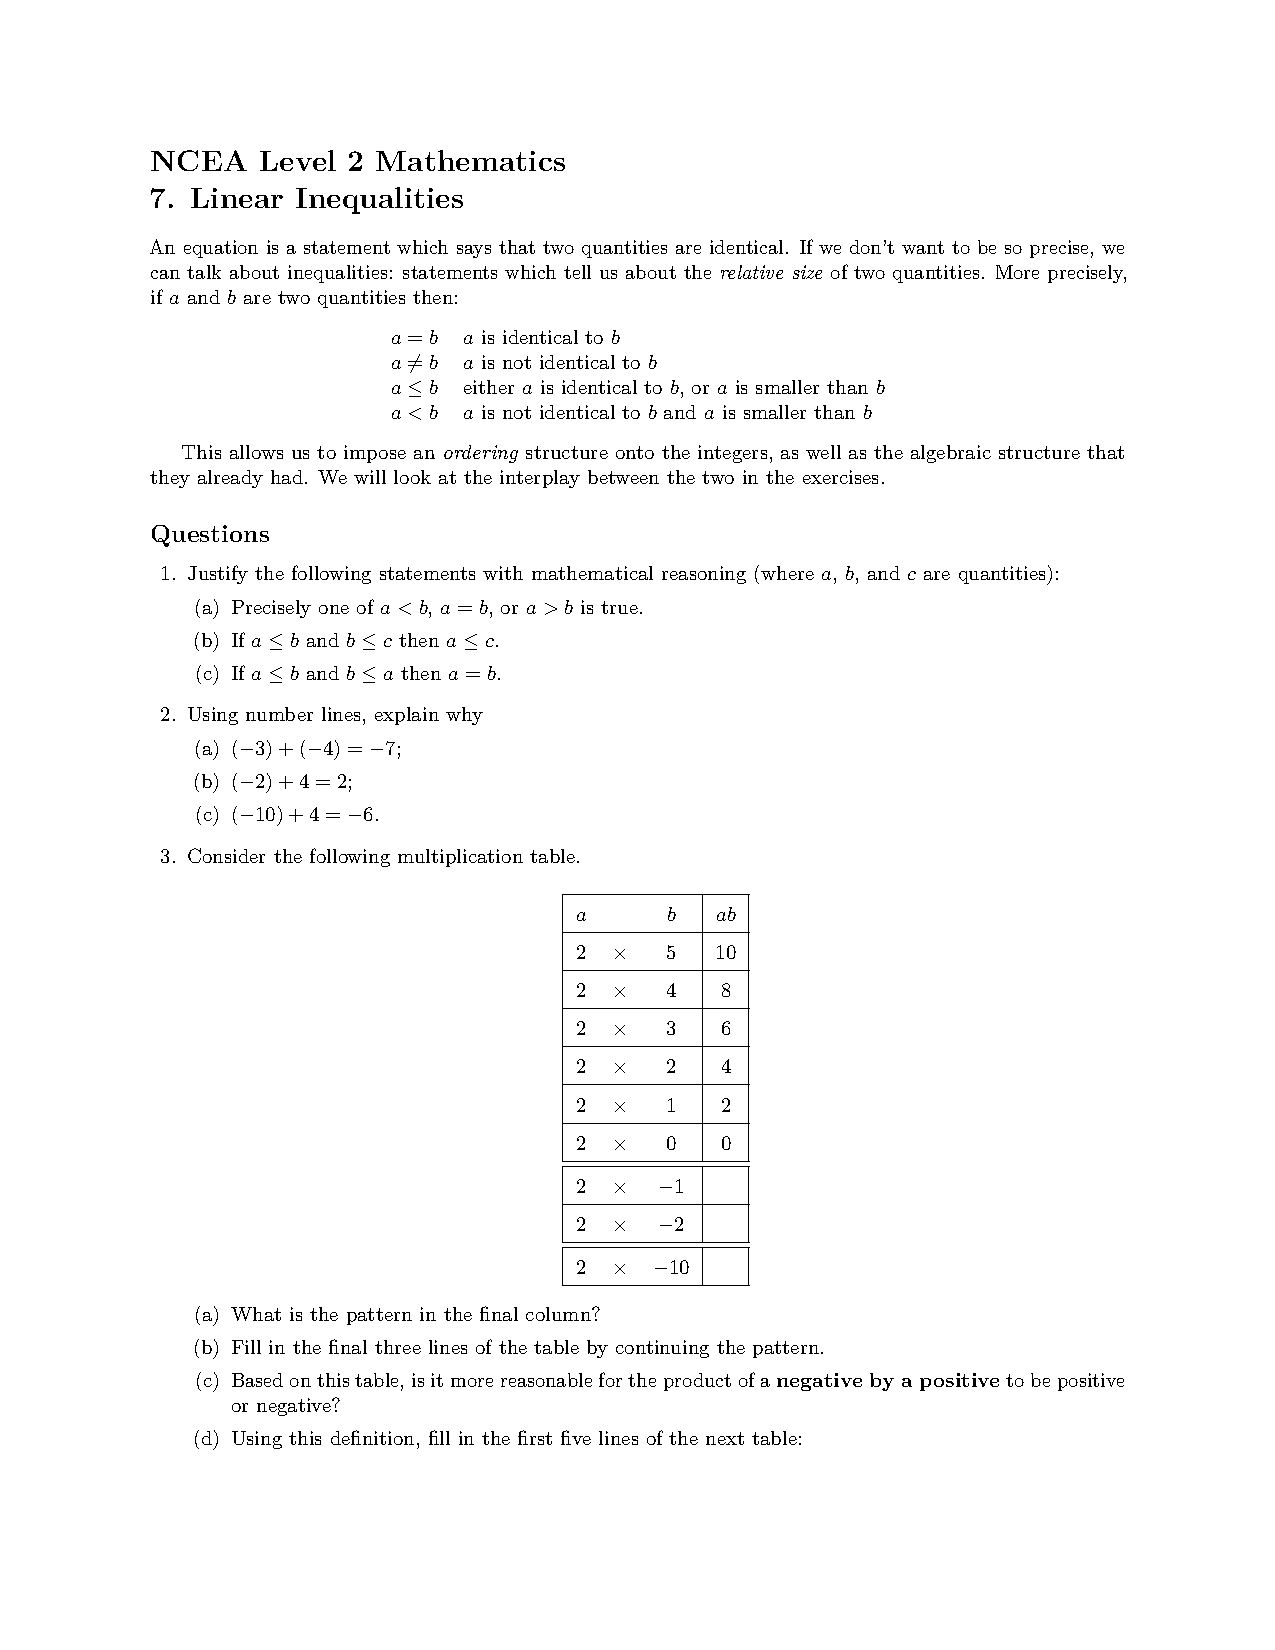
\includepdf[pages={-},pagecommand={}]{07-inequalities.pdf}
  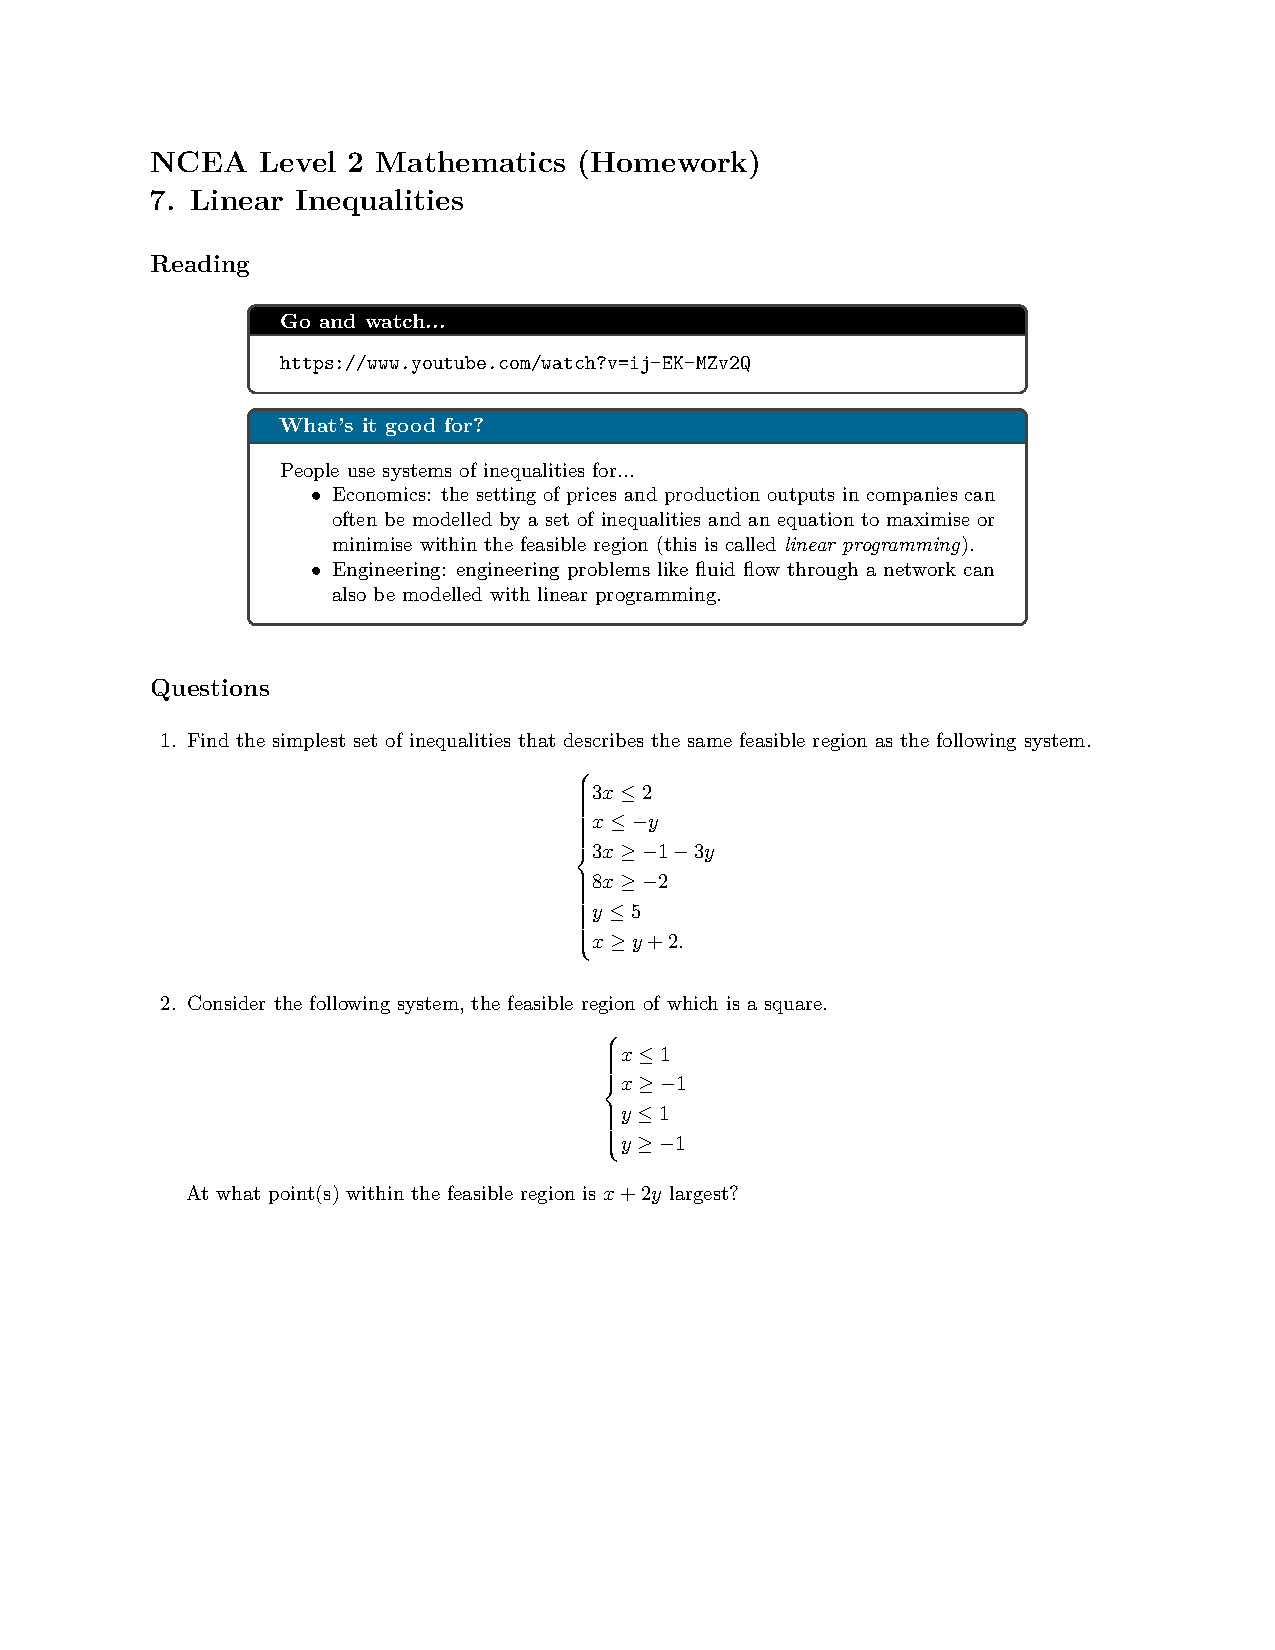
\includepdf[pages={-},pagecommand={}]{07-inequalities-hw.pdf}
  \phantomsection\addcontentsline{toc}{section}{The Quadratic Formula}
  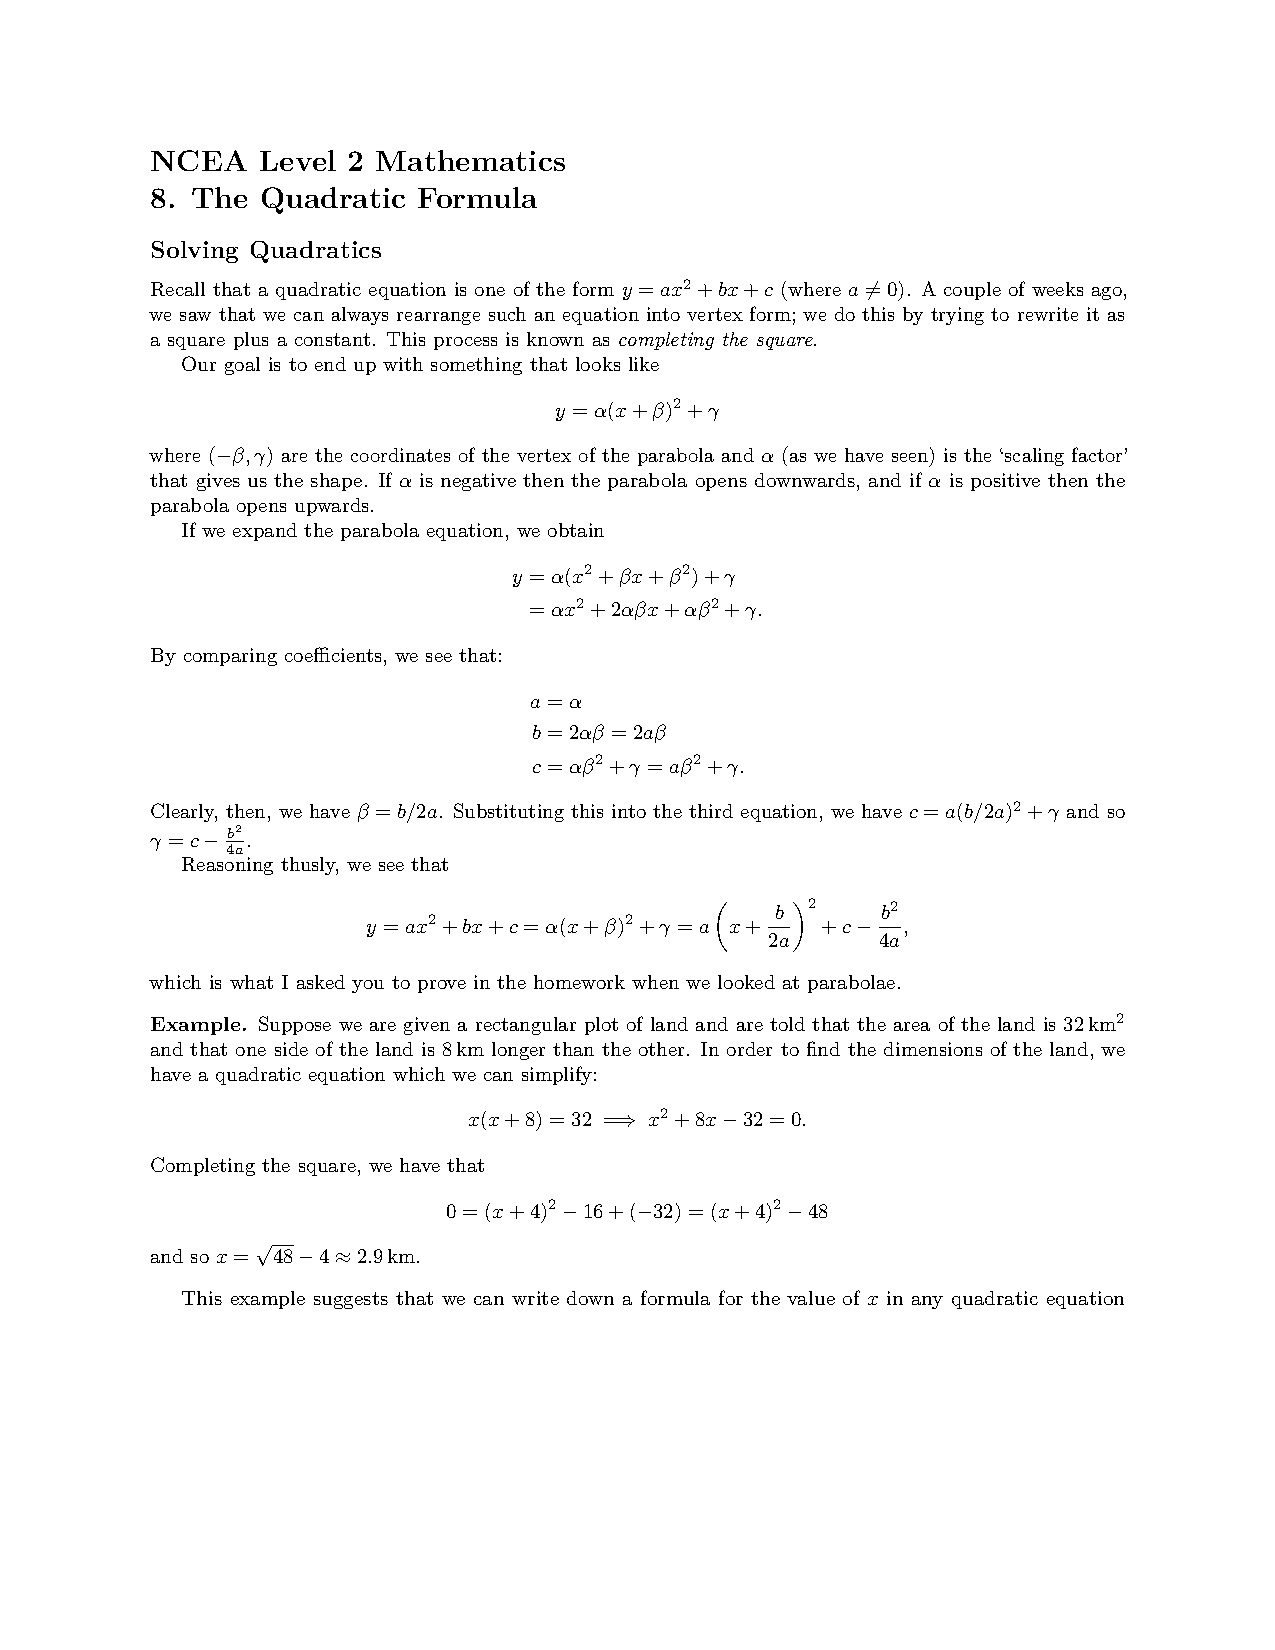
\includepdf[pages={-},pagecommand={}]{08-quadratics2.pdf}
  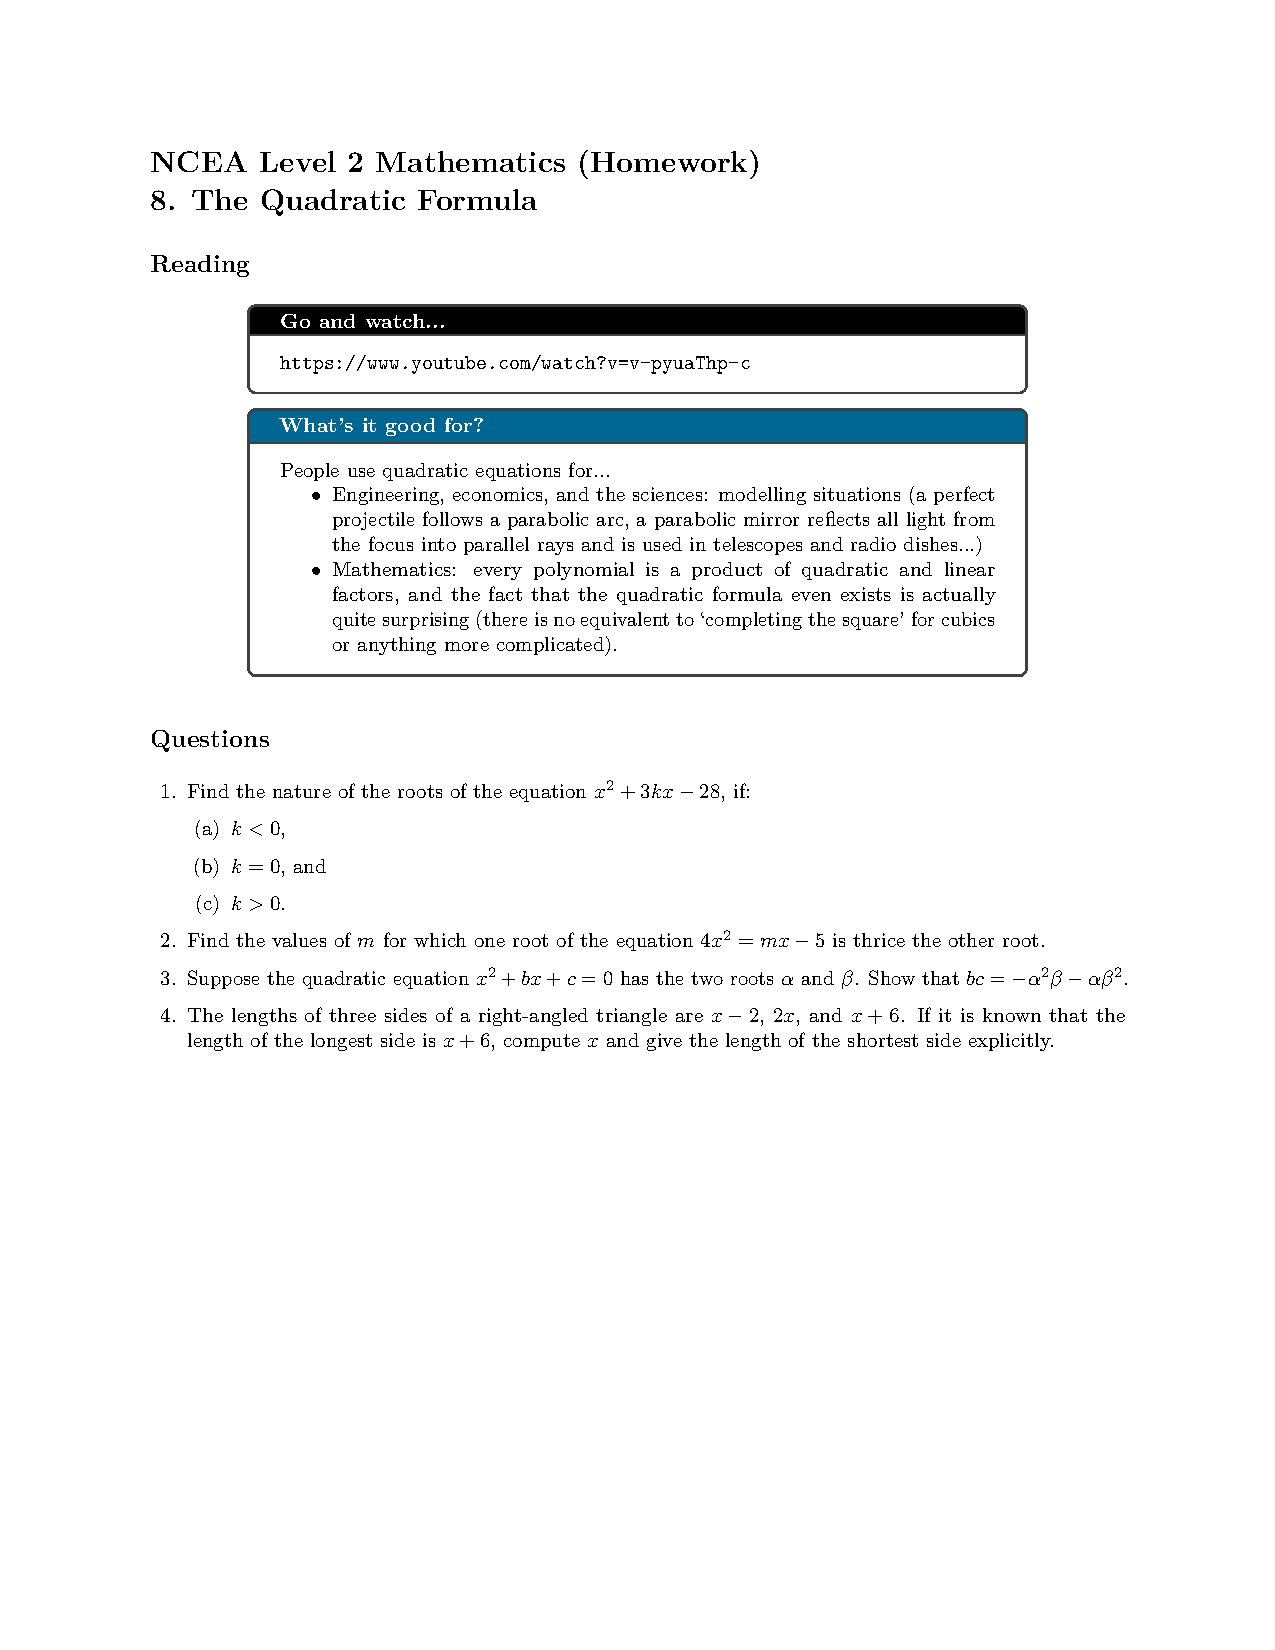
\includepdf[pages={-},pagecommand={}]{08-quadratics2-hw.pdf}
  \phantomsection\addcontentsline{toc}{section}{Exponential and Logarithmic Functions}
  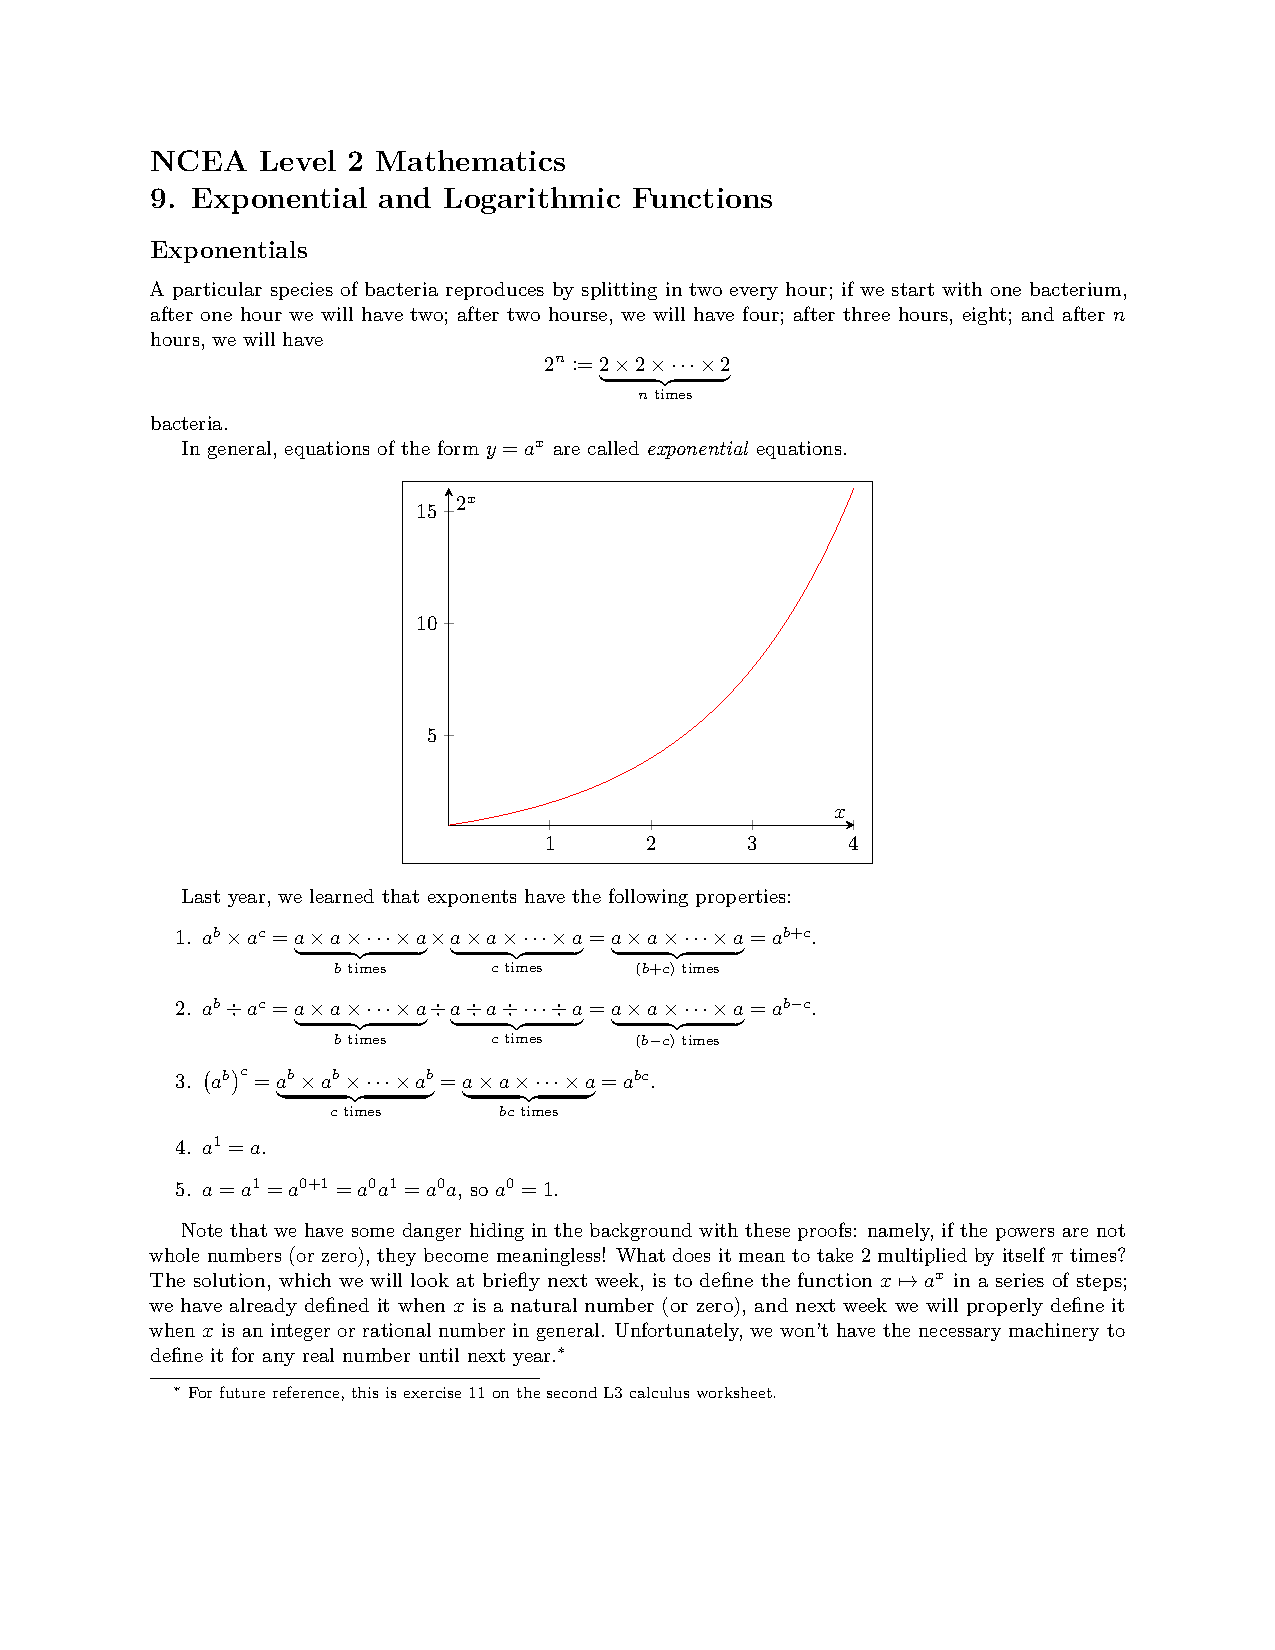
\includepdf[pages={-},pagecommand={}]{09-exponentials.pdf}
  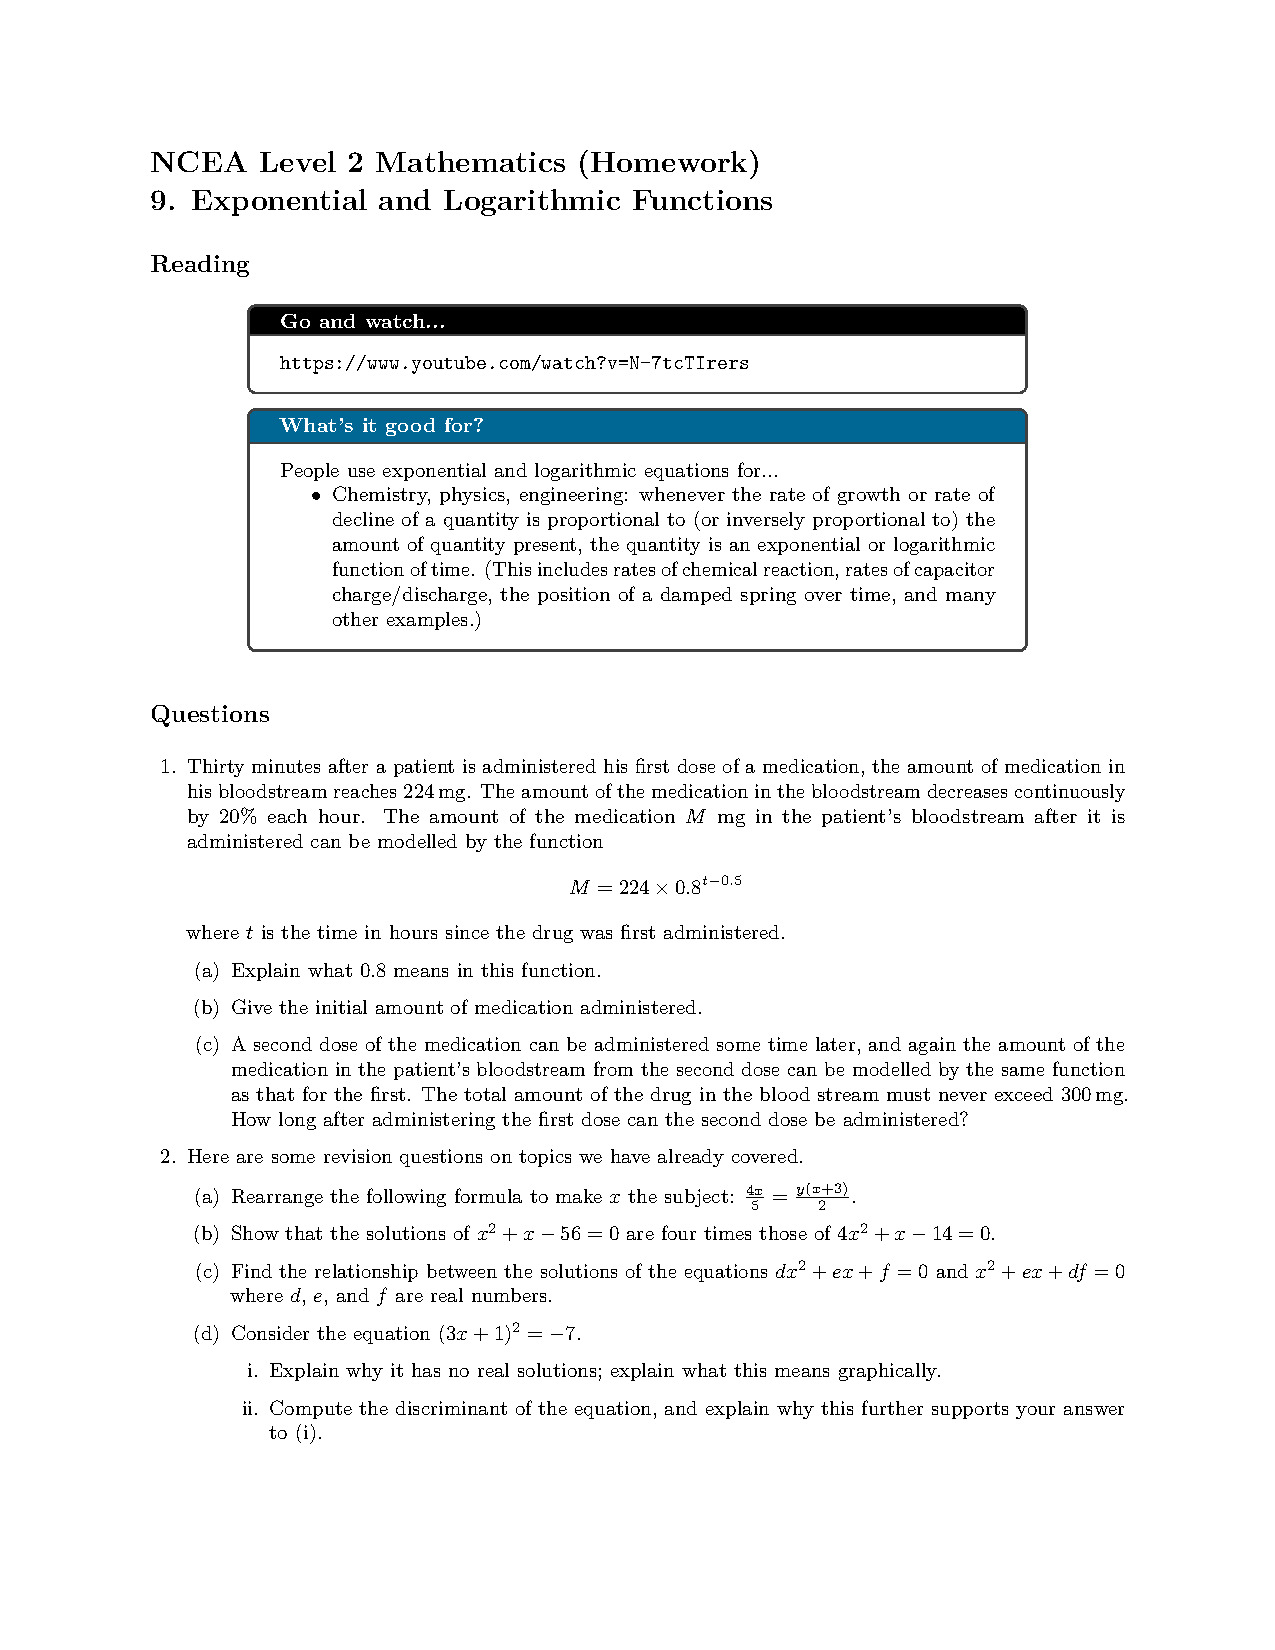
\includepdf[pages={-},pagecommand={}]{09-exponentials-hw.pdf}
  \phantomsection\addcontentsline{toc}{section}{Negative and Fractional Powers}
  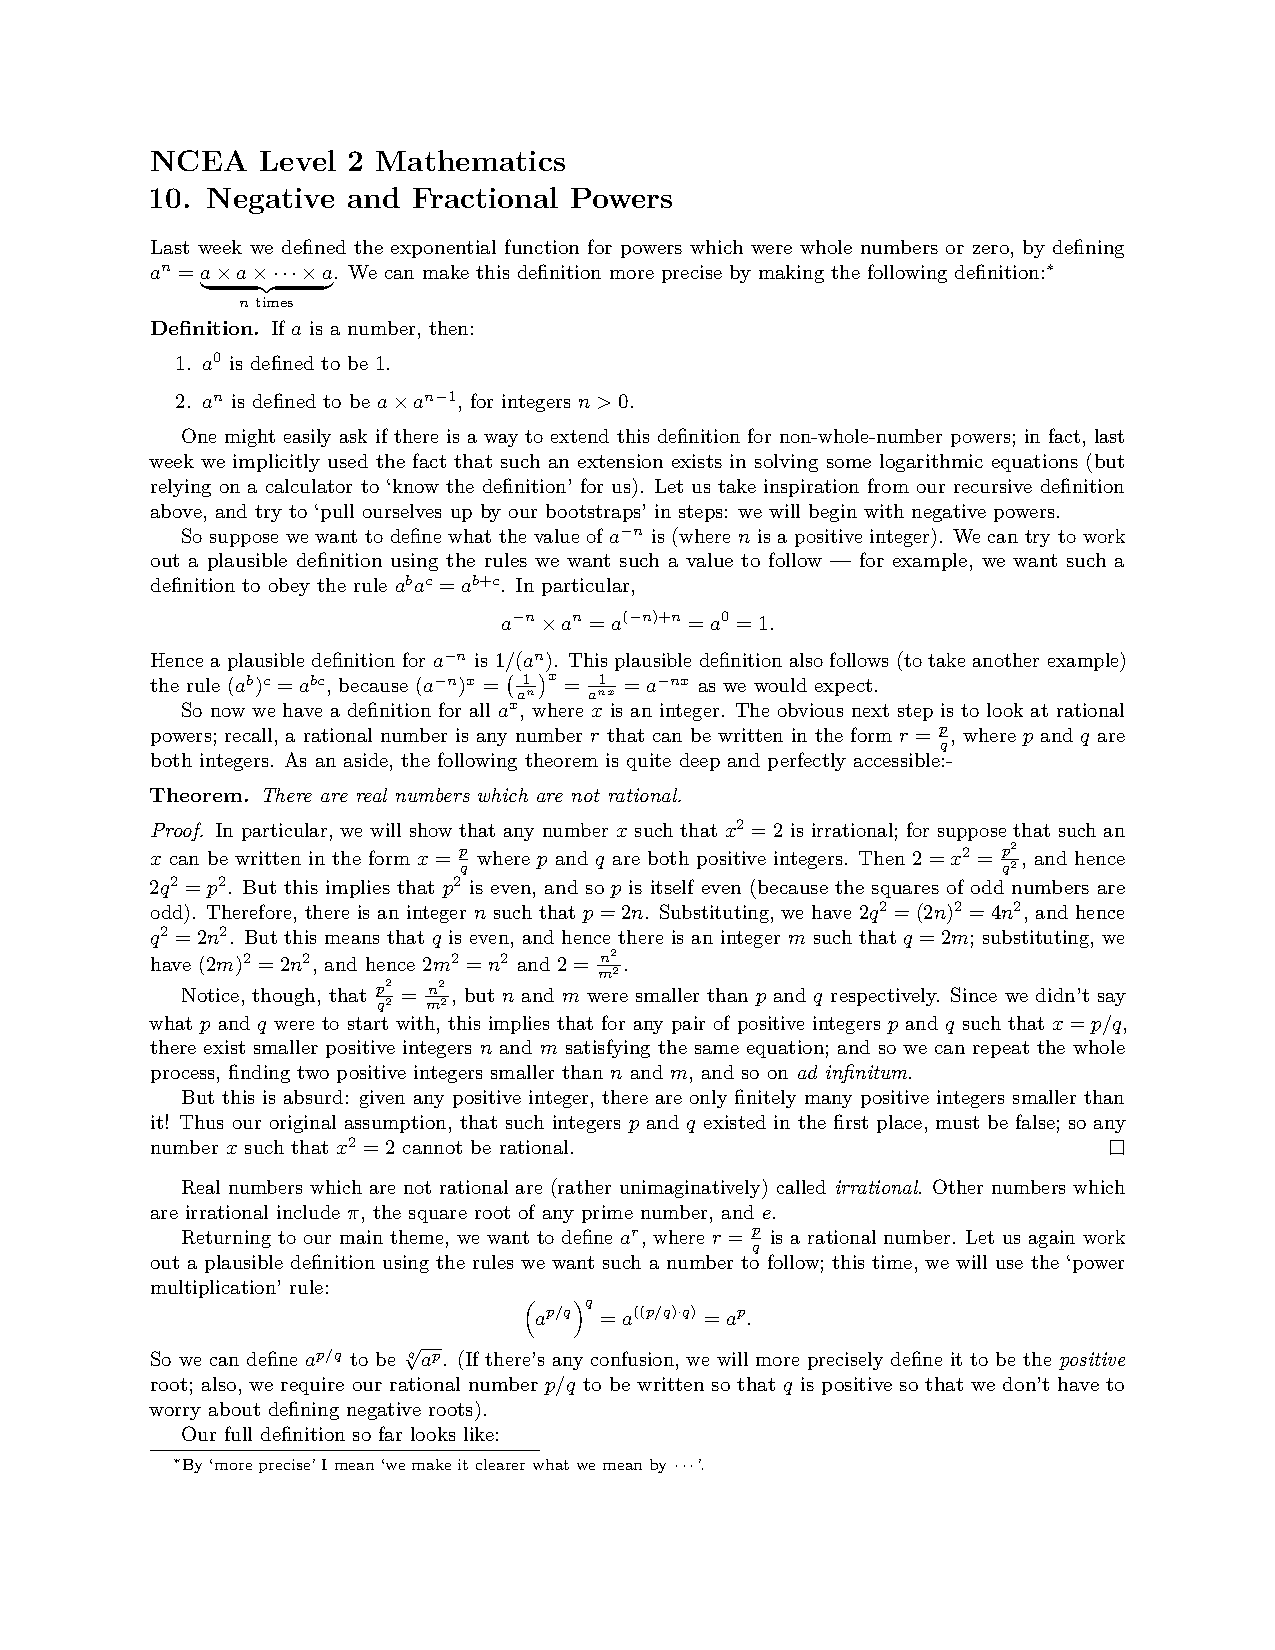
\includepdf[pages={-},pagecommand={}]{10-radicals.pdf}
  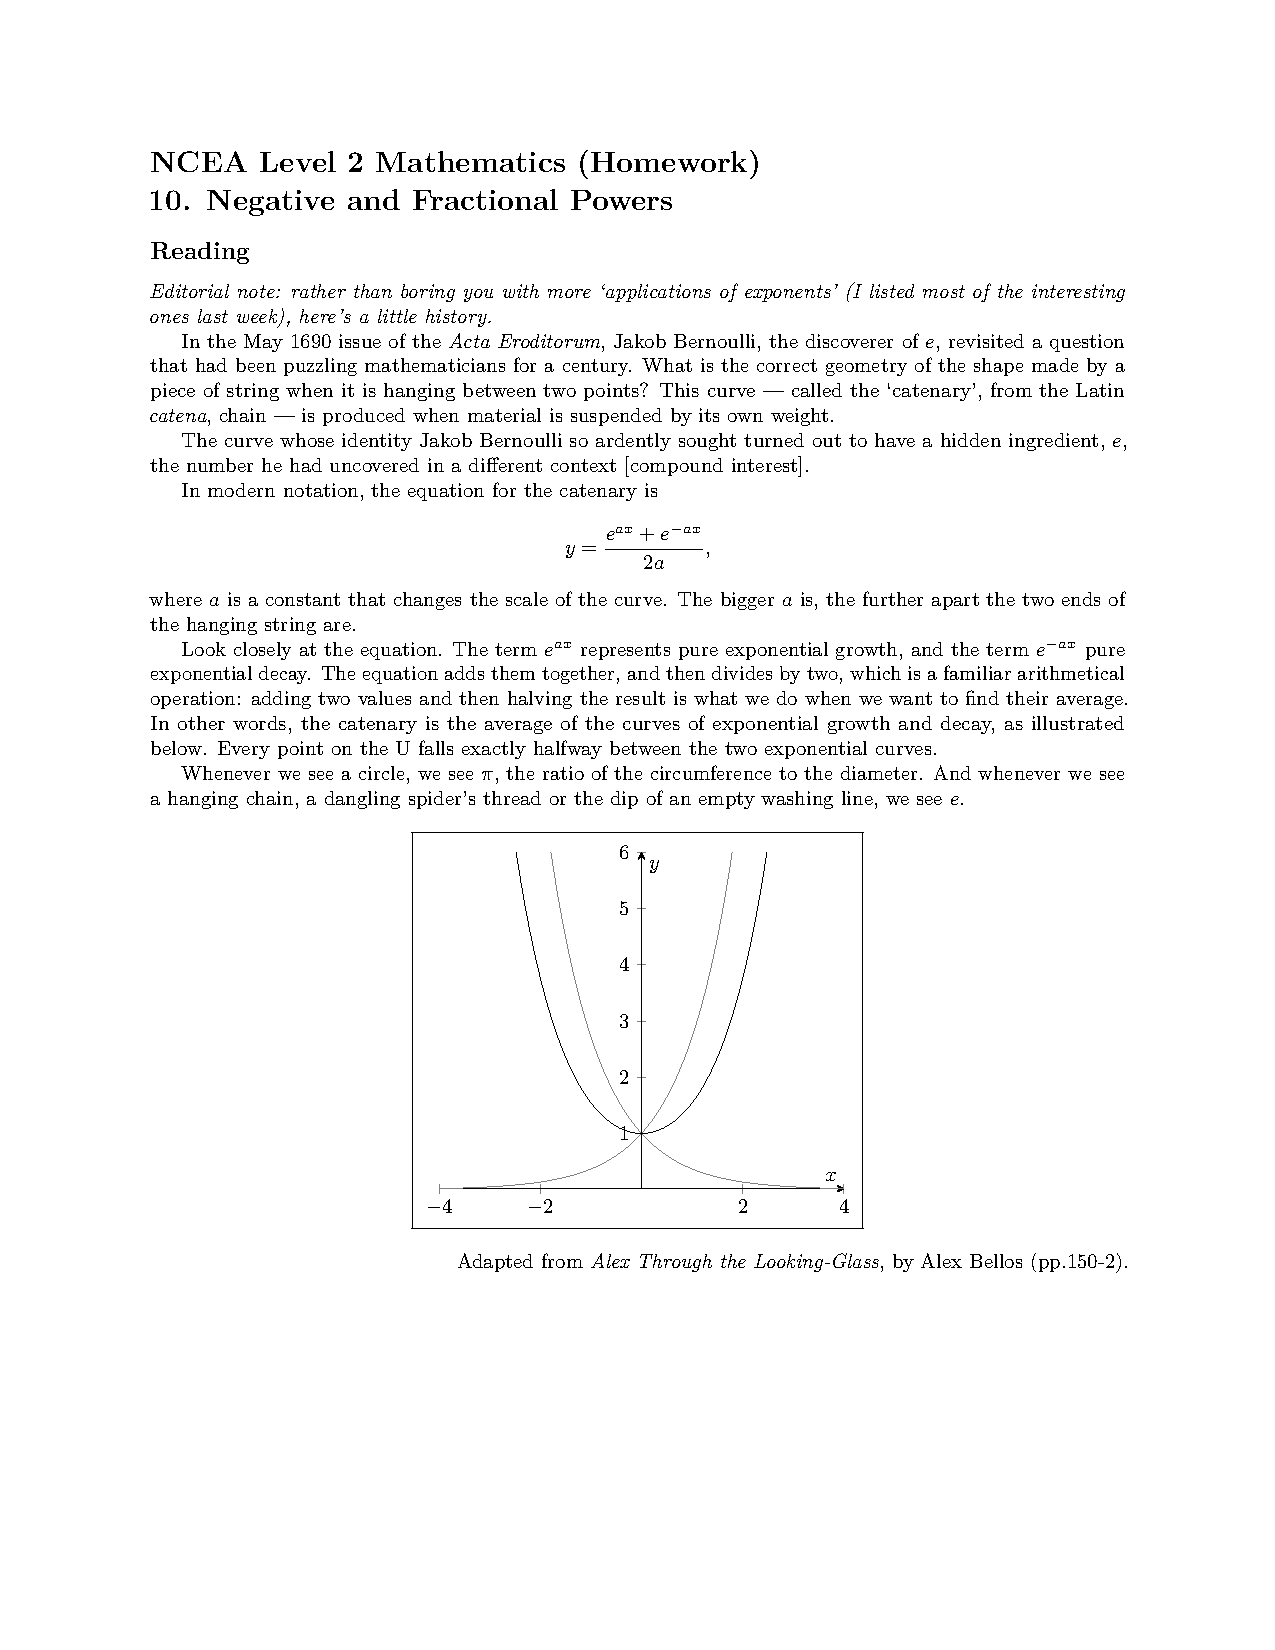
\includepdf[pages={-},pagecommand={}]{10-radicals-hw.pdf}

  \chapter{Calculus}
  \phantomsection\addcontentsline{toc}{section}{Slopes and Differentiation}
  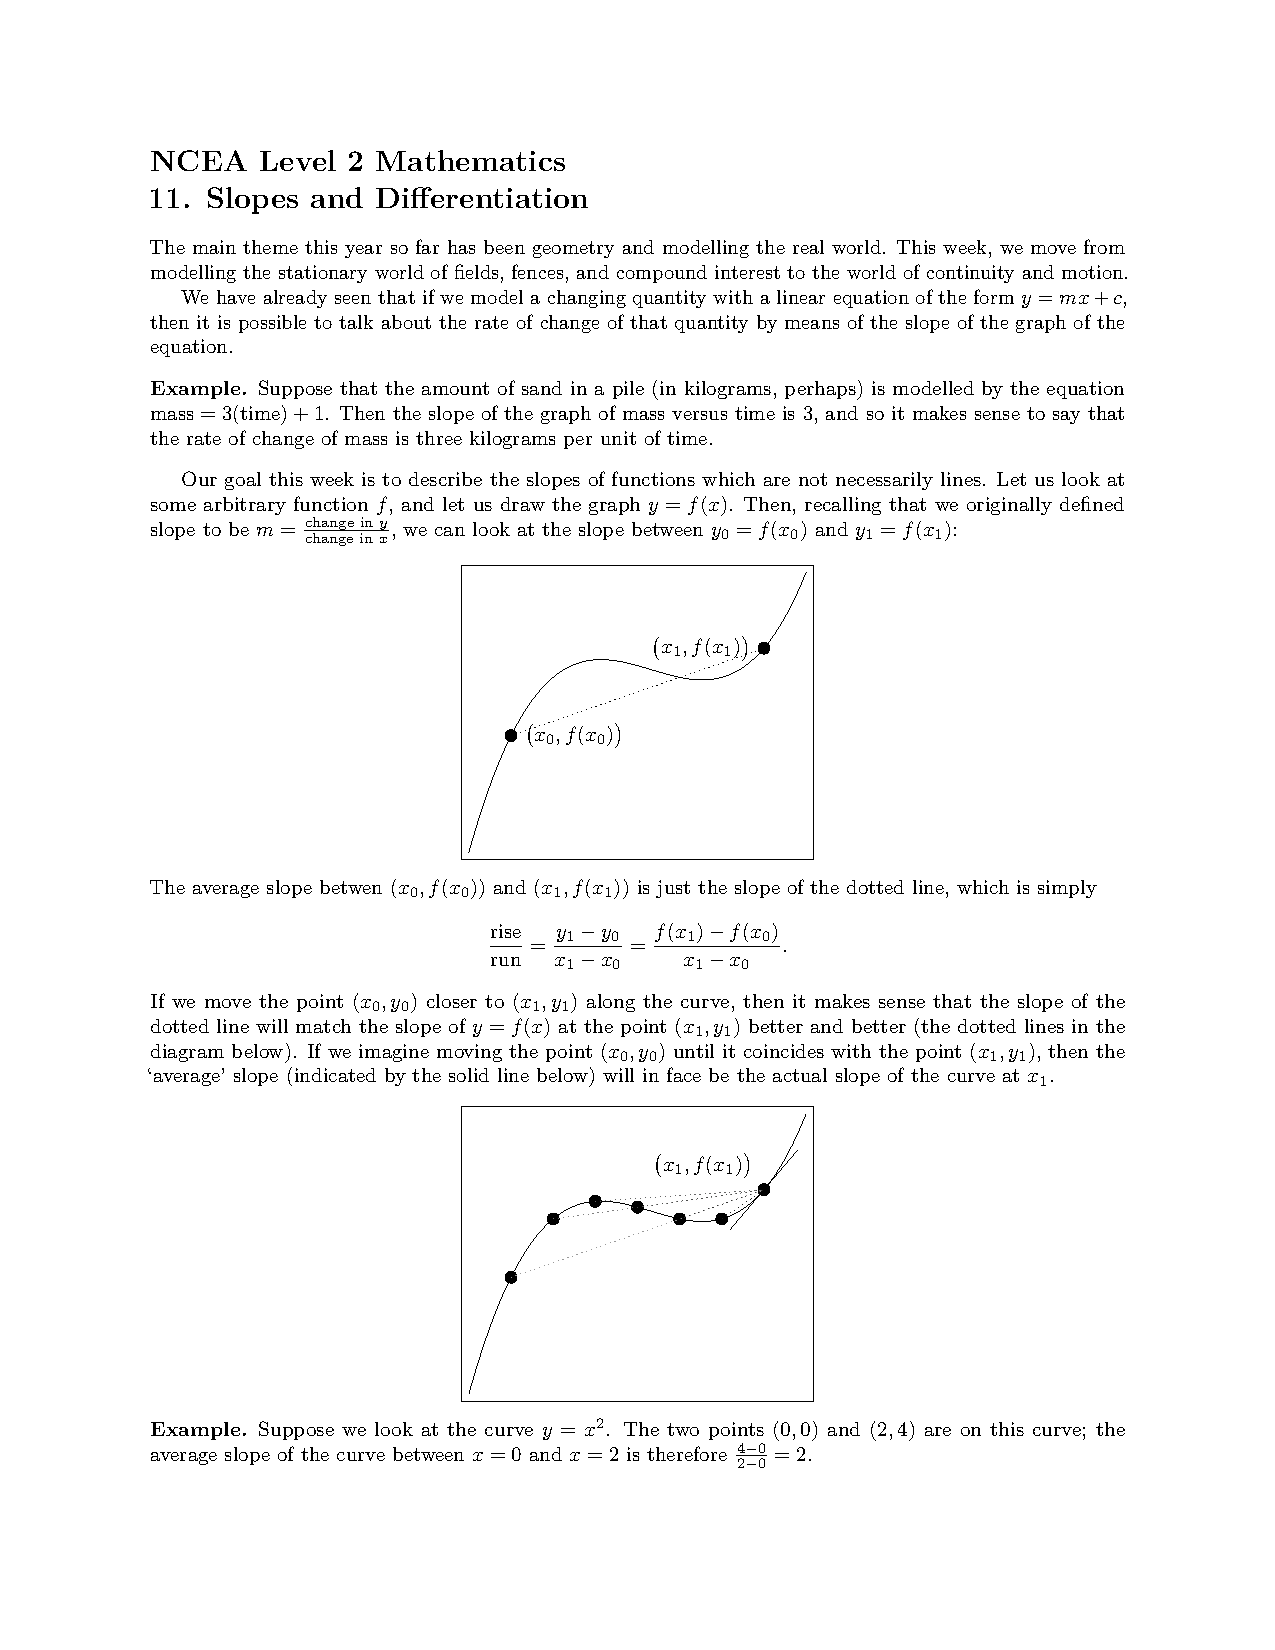
\includepdf[pages={-},pagecommand={}]{11-slopes.pdf}
  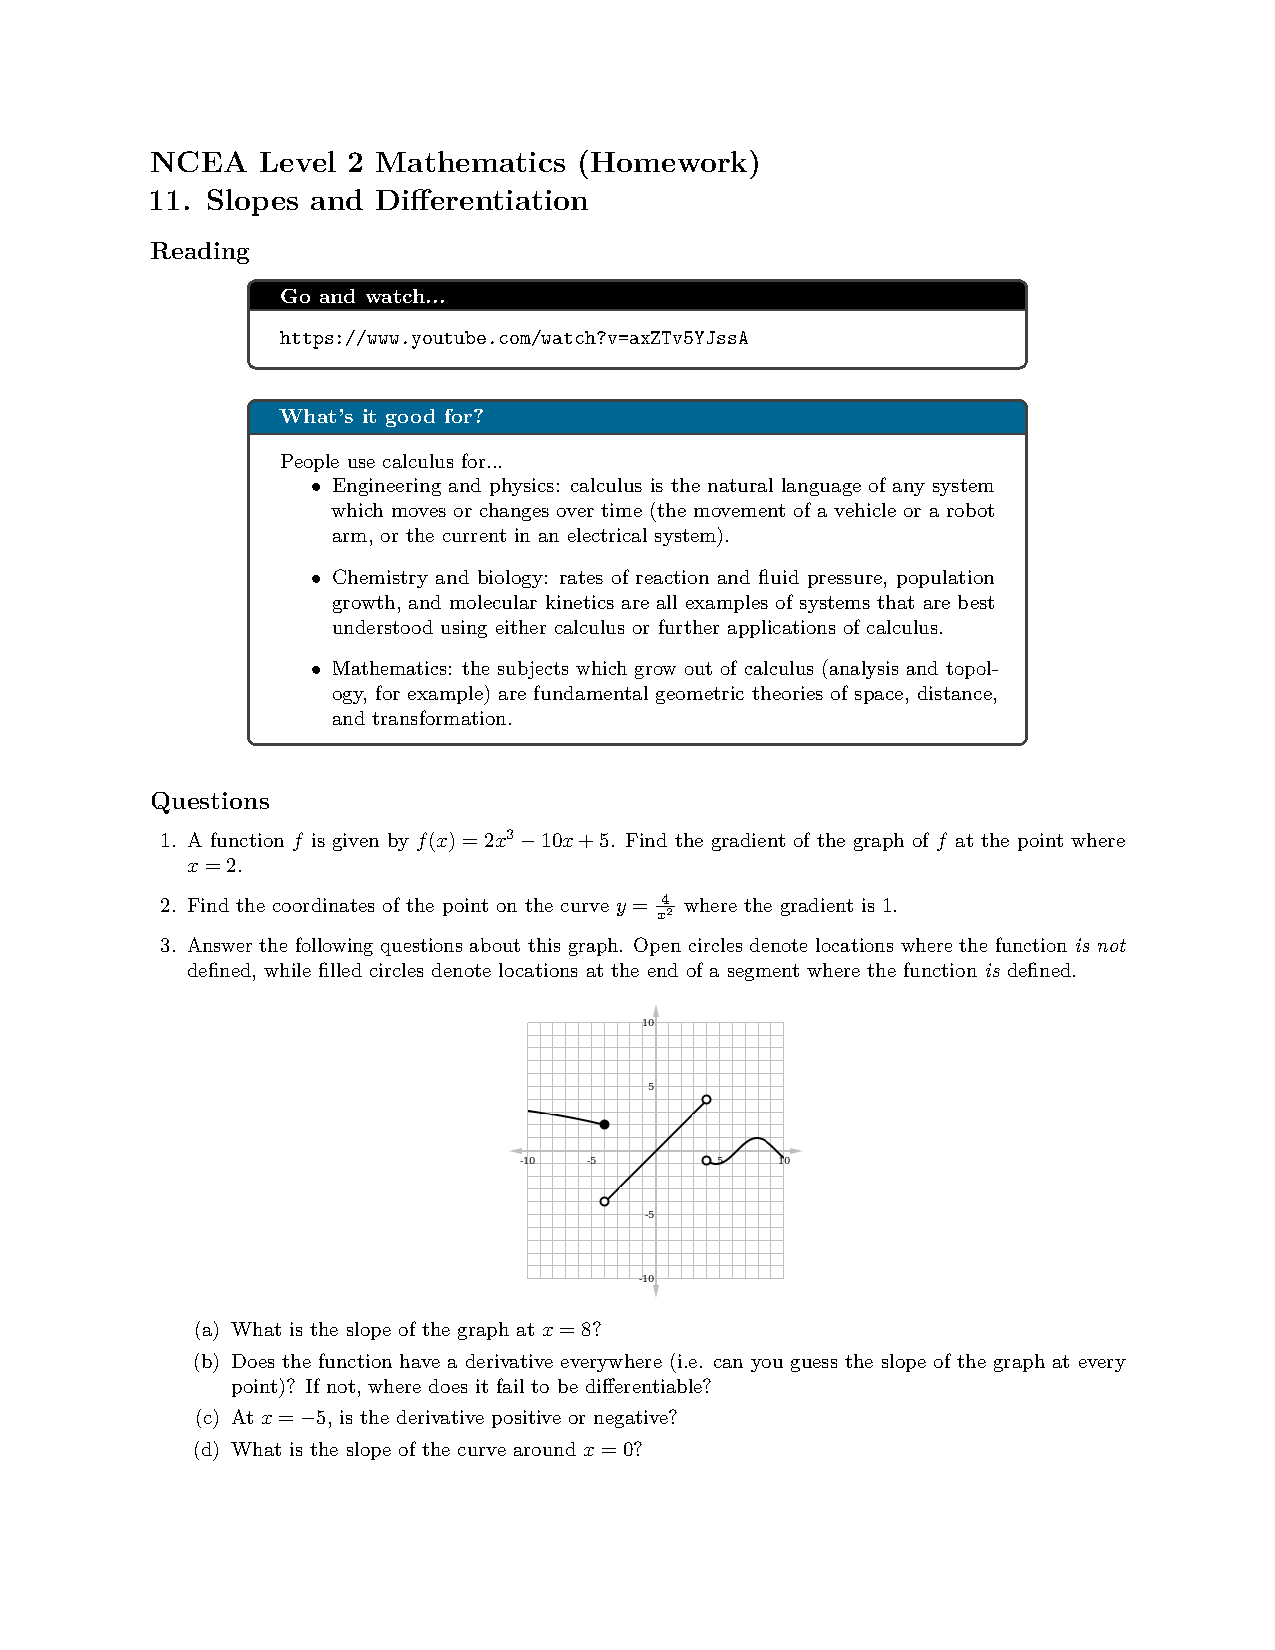
\includepdf[pages={-},pagecommand={}]{11-slopes-hw.pdf}
  \phantomsection\addcontentsline{toc}{section}{Tangent Lines and Approximations}
  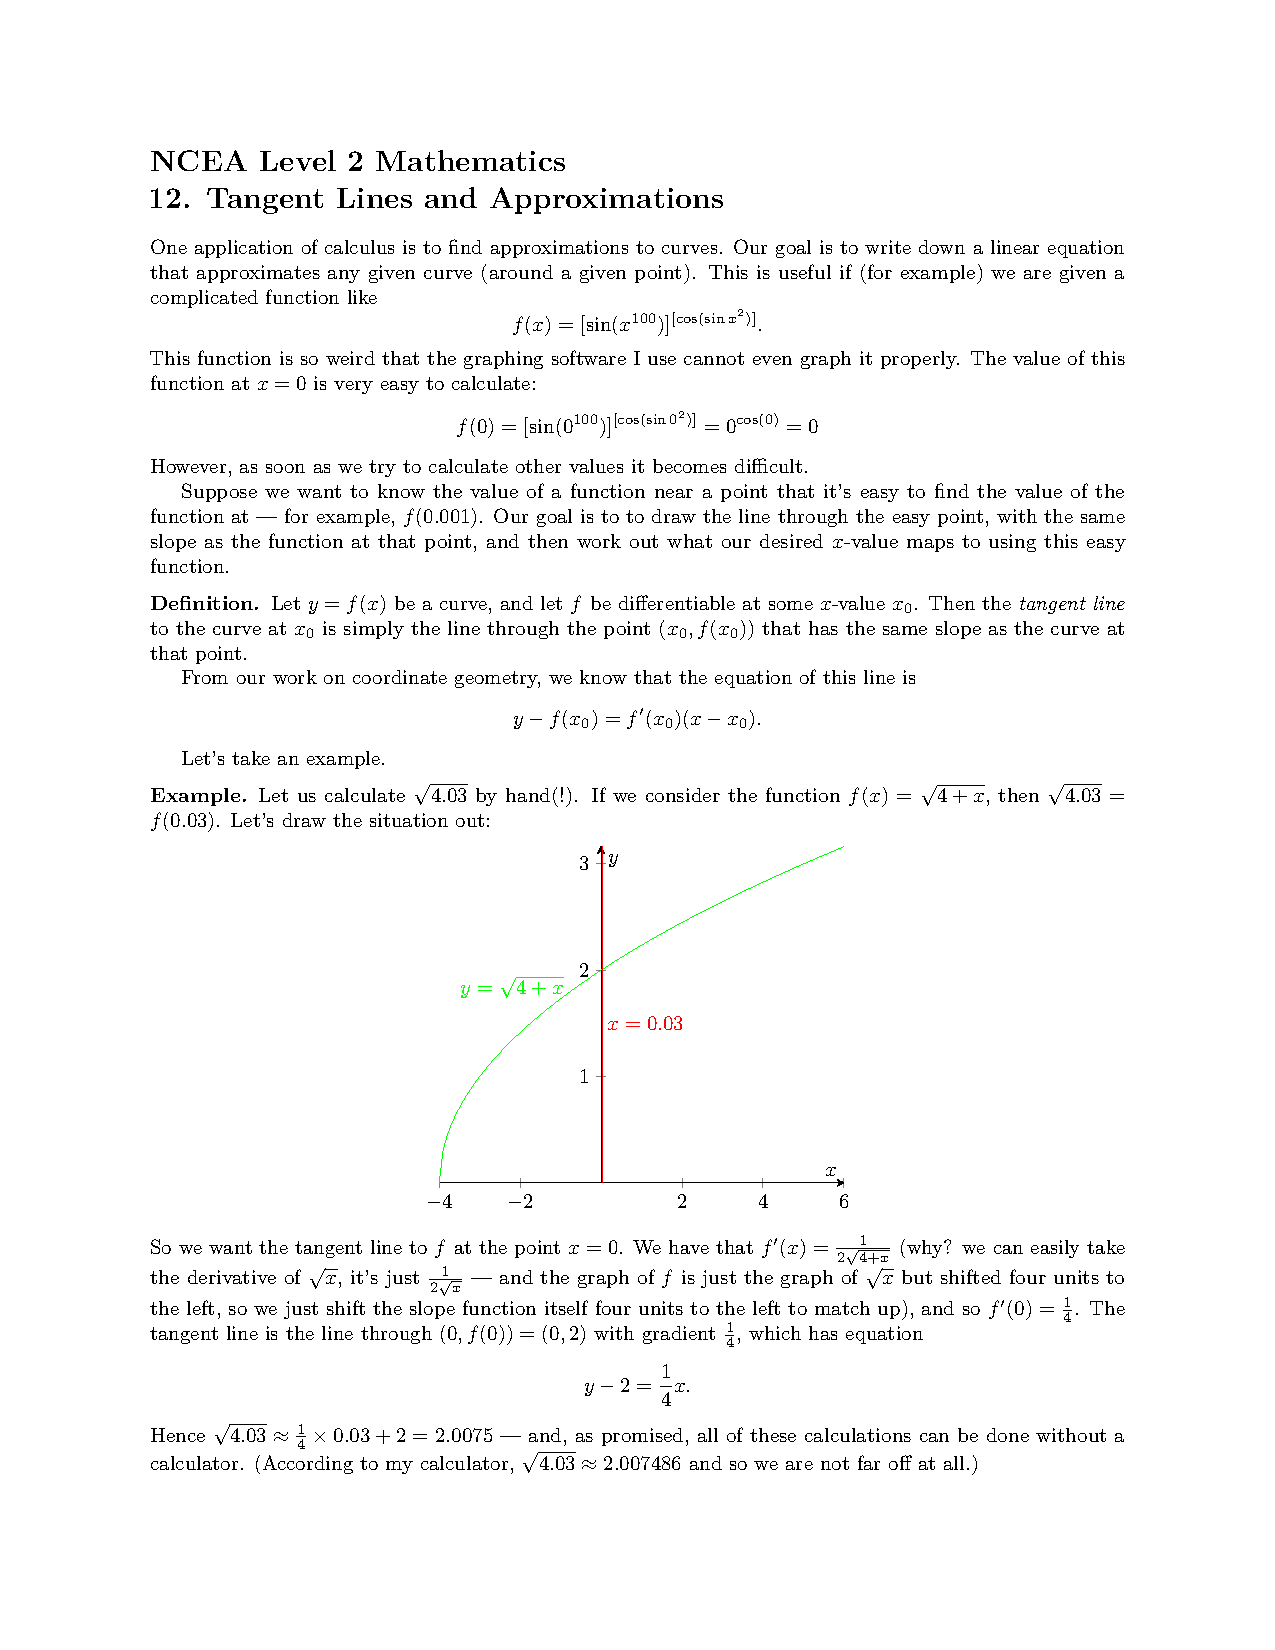
\includepdf[pages={-},pagecommand={}]{12-tangents.pdf}
  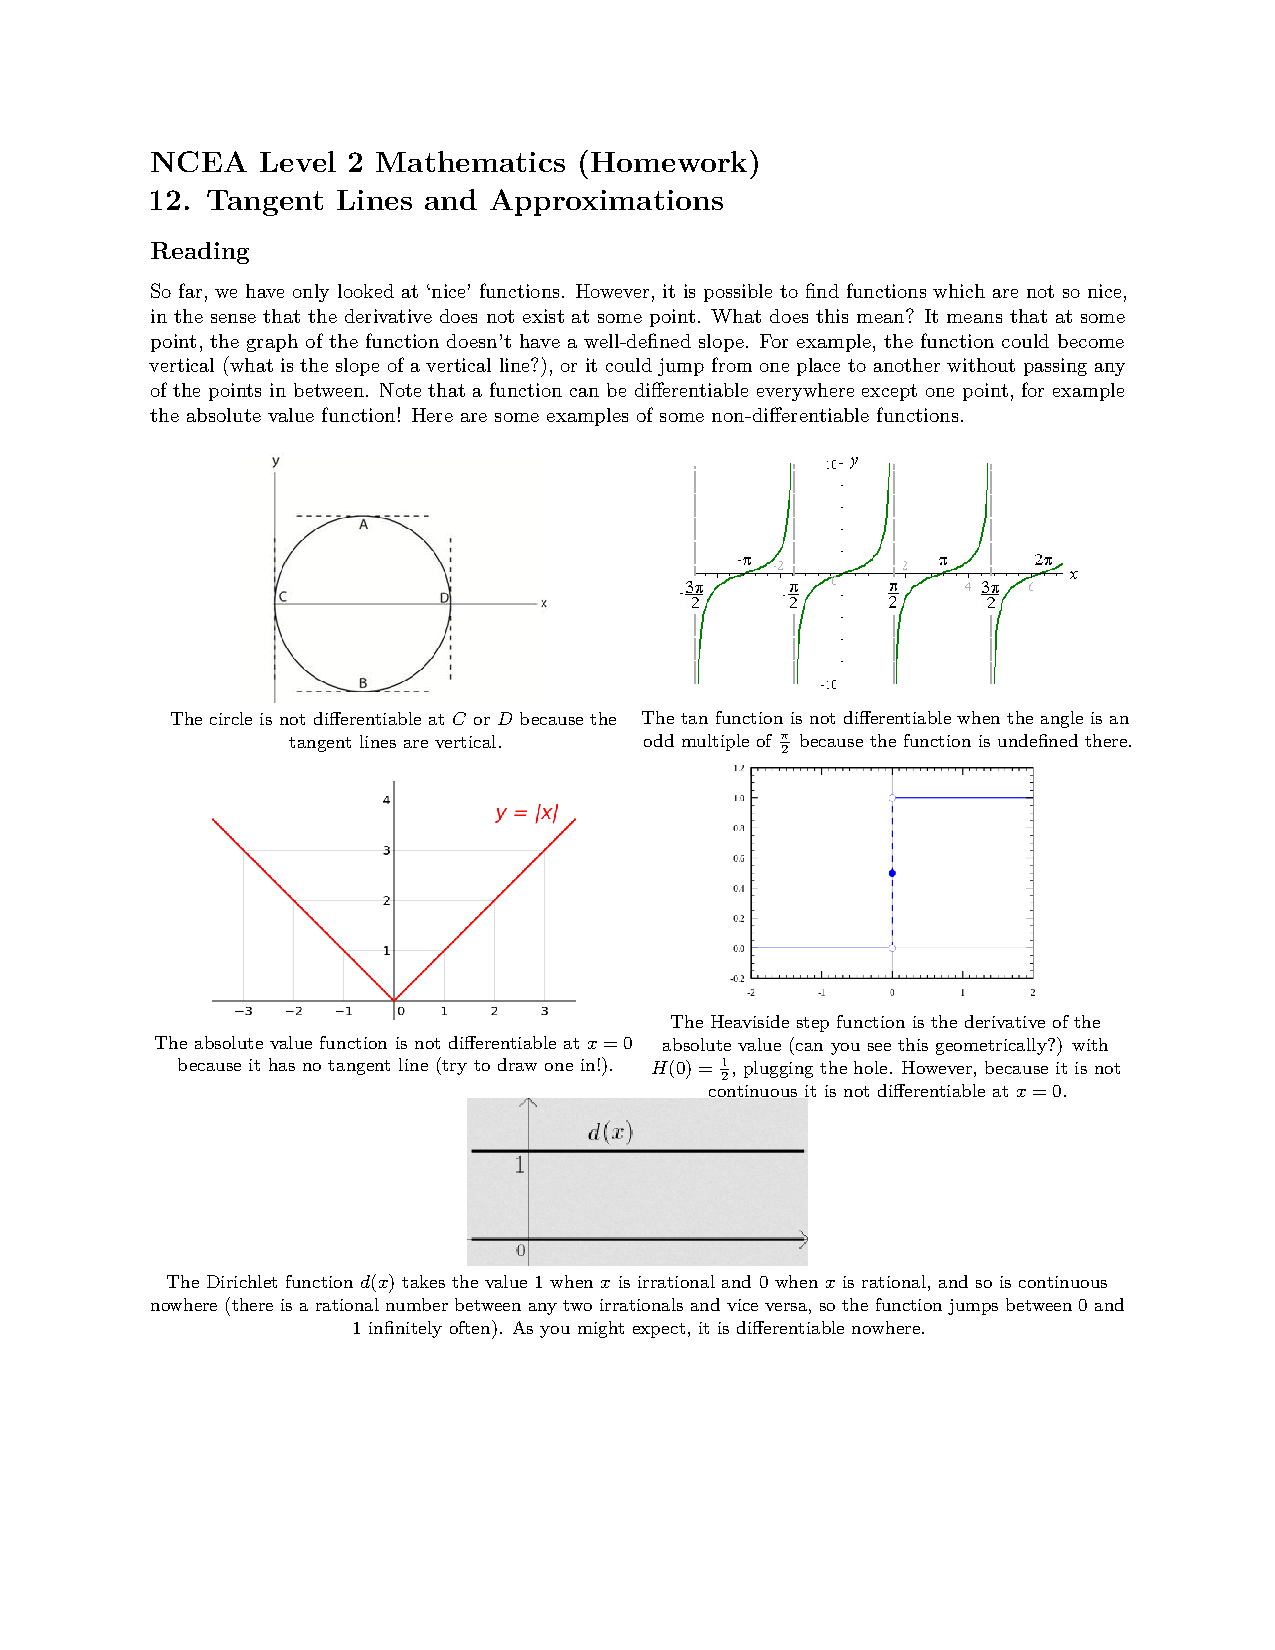
\includepdf[pages={-},pagecommand={}]{12-tangents-hw.pdf}
  \phantomsection\addcontentsline{toc}{section}{Turning Points and Optimisation}
  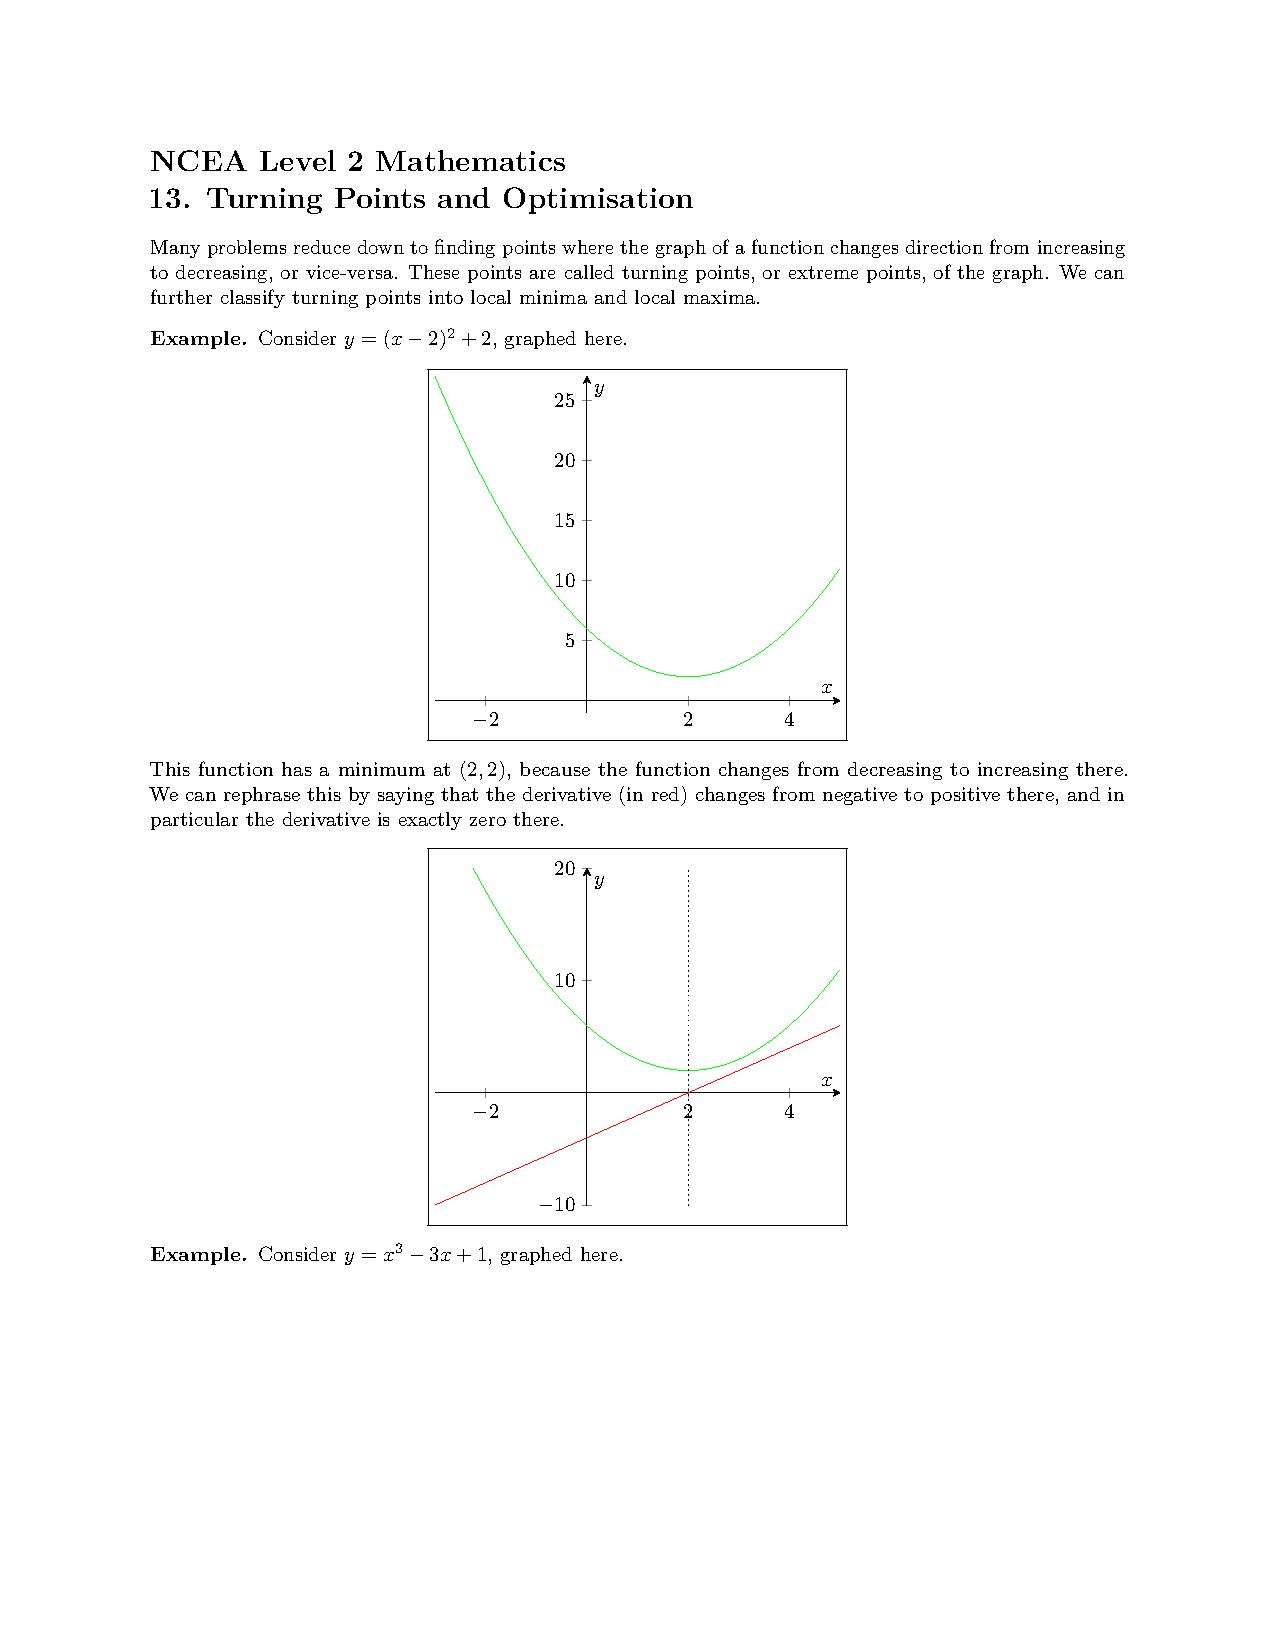
\includepdf[pages={-},pagecommand={}]{13-optimisation.pdf}
  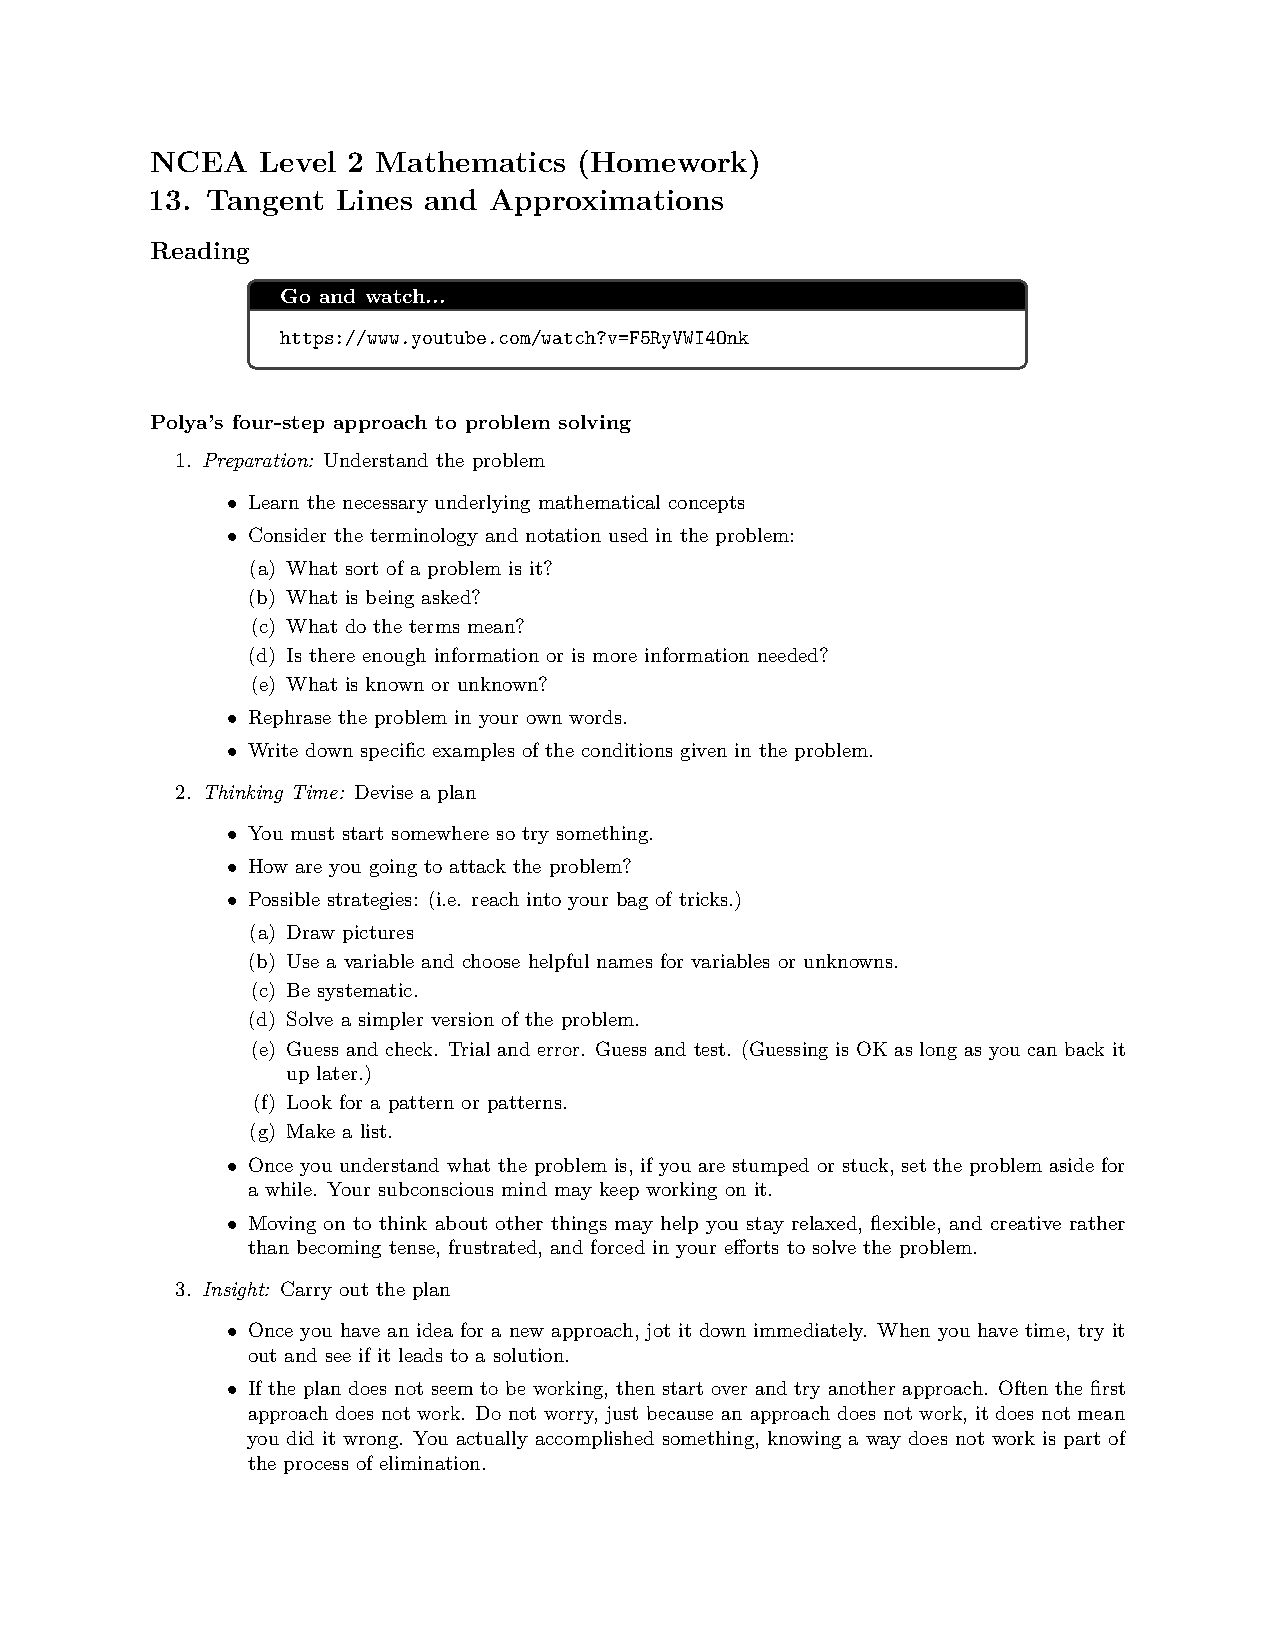
\includepdf[pages={-},pagecommand={}]{13-optimisation-hw.pdf}
  \phantomsection\addcontentsline{toc}{section}{Anti-differentiation}
  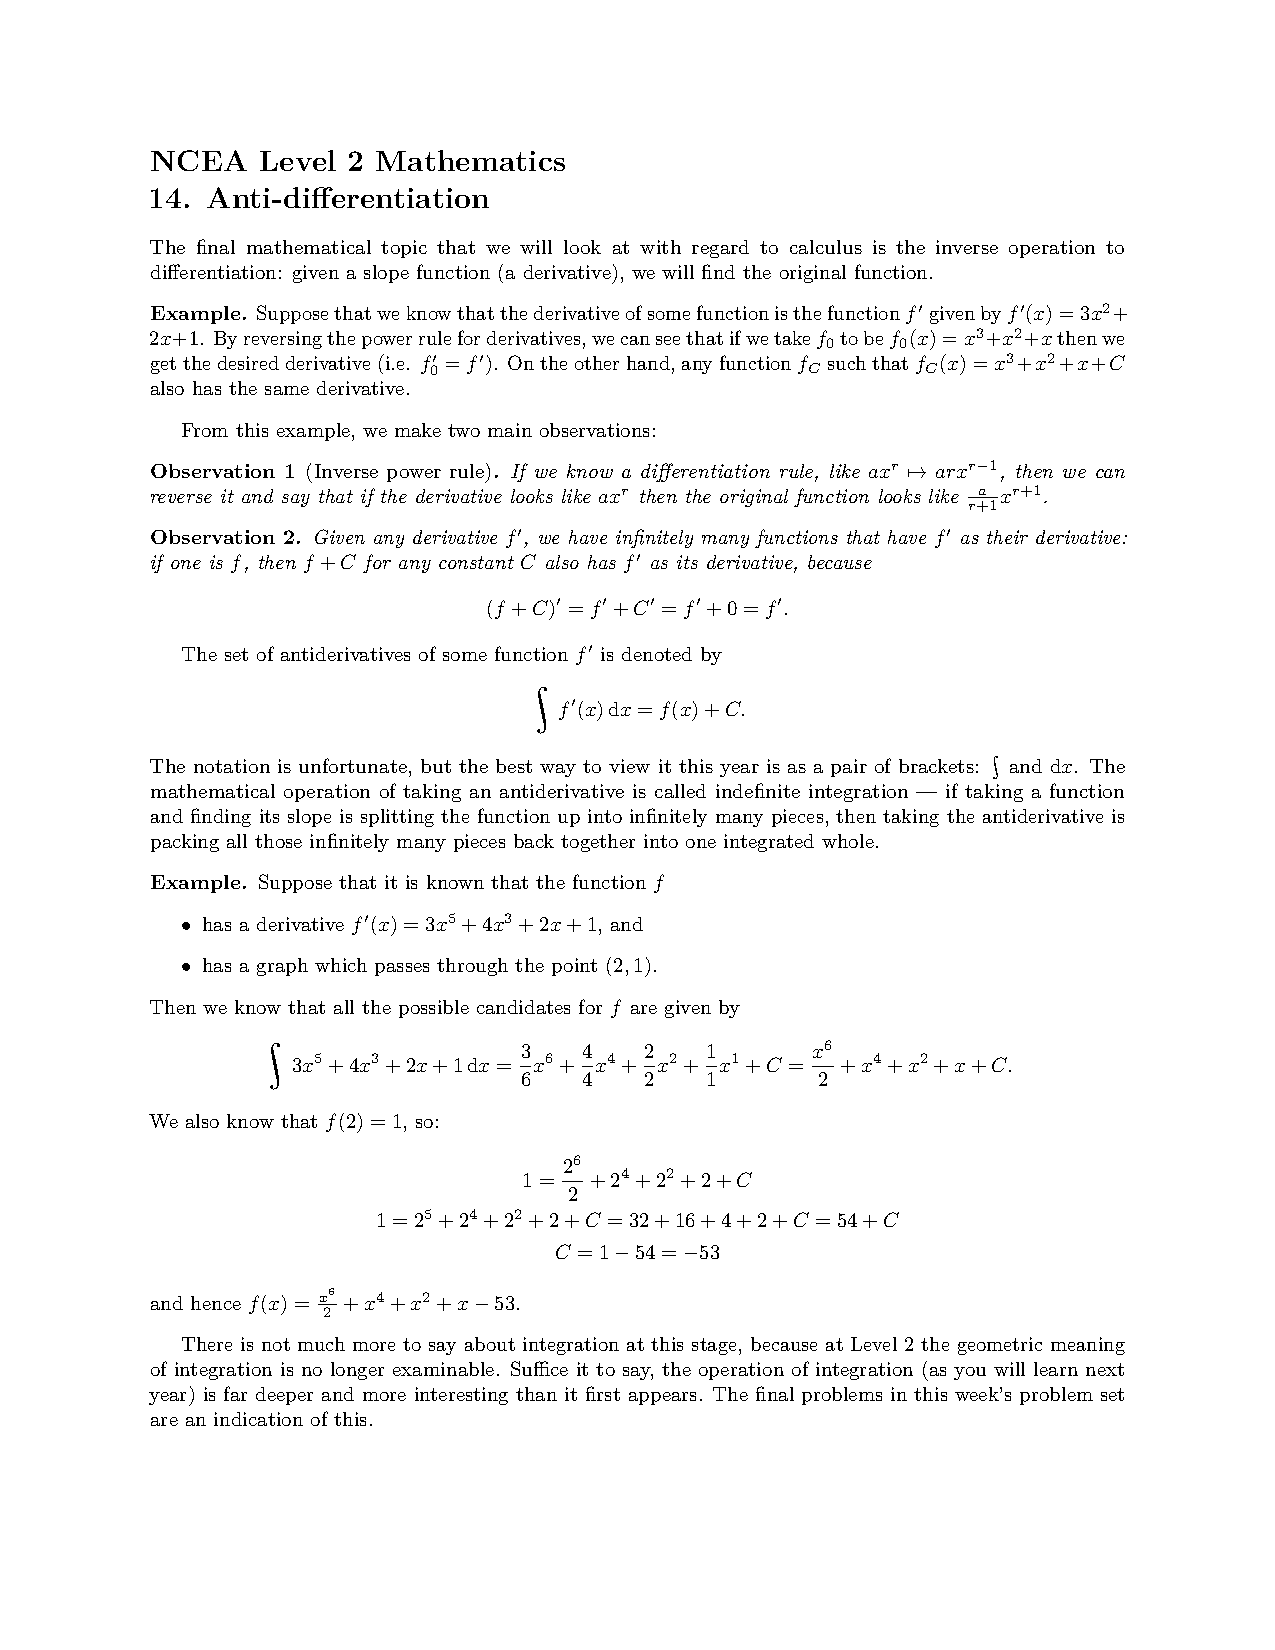
\includepdf[pages={-},pagecommand={}]{14-antidifferentiation.pdf}
  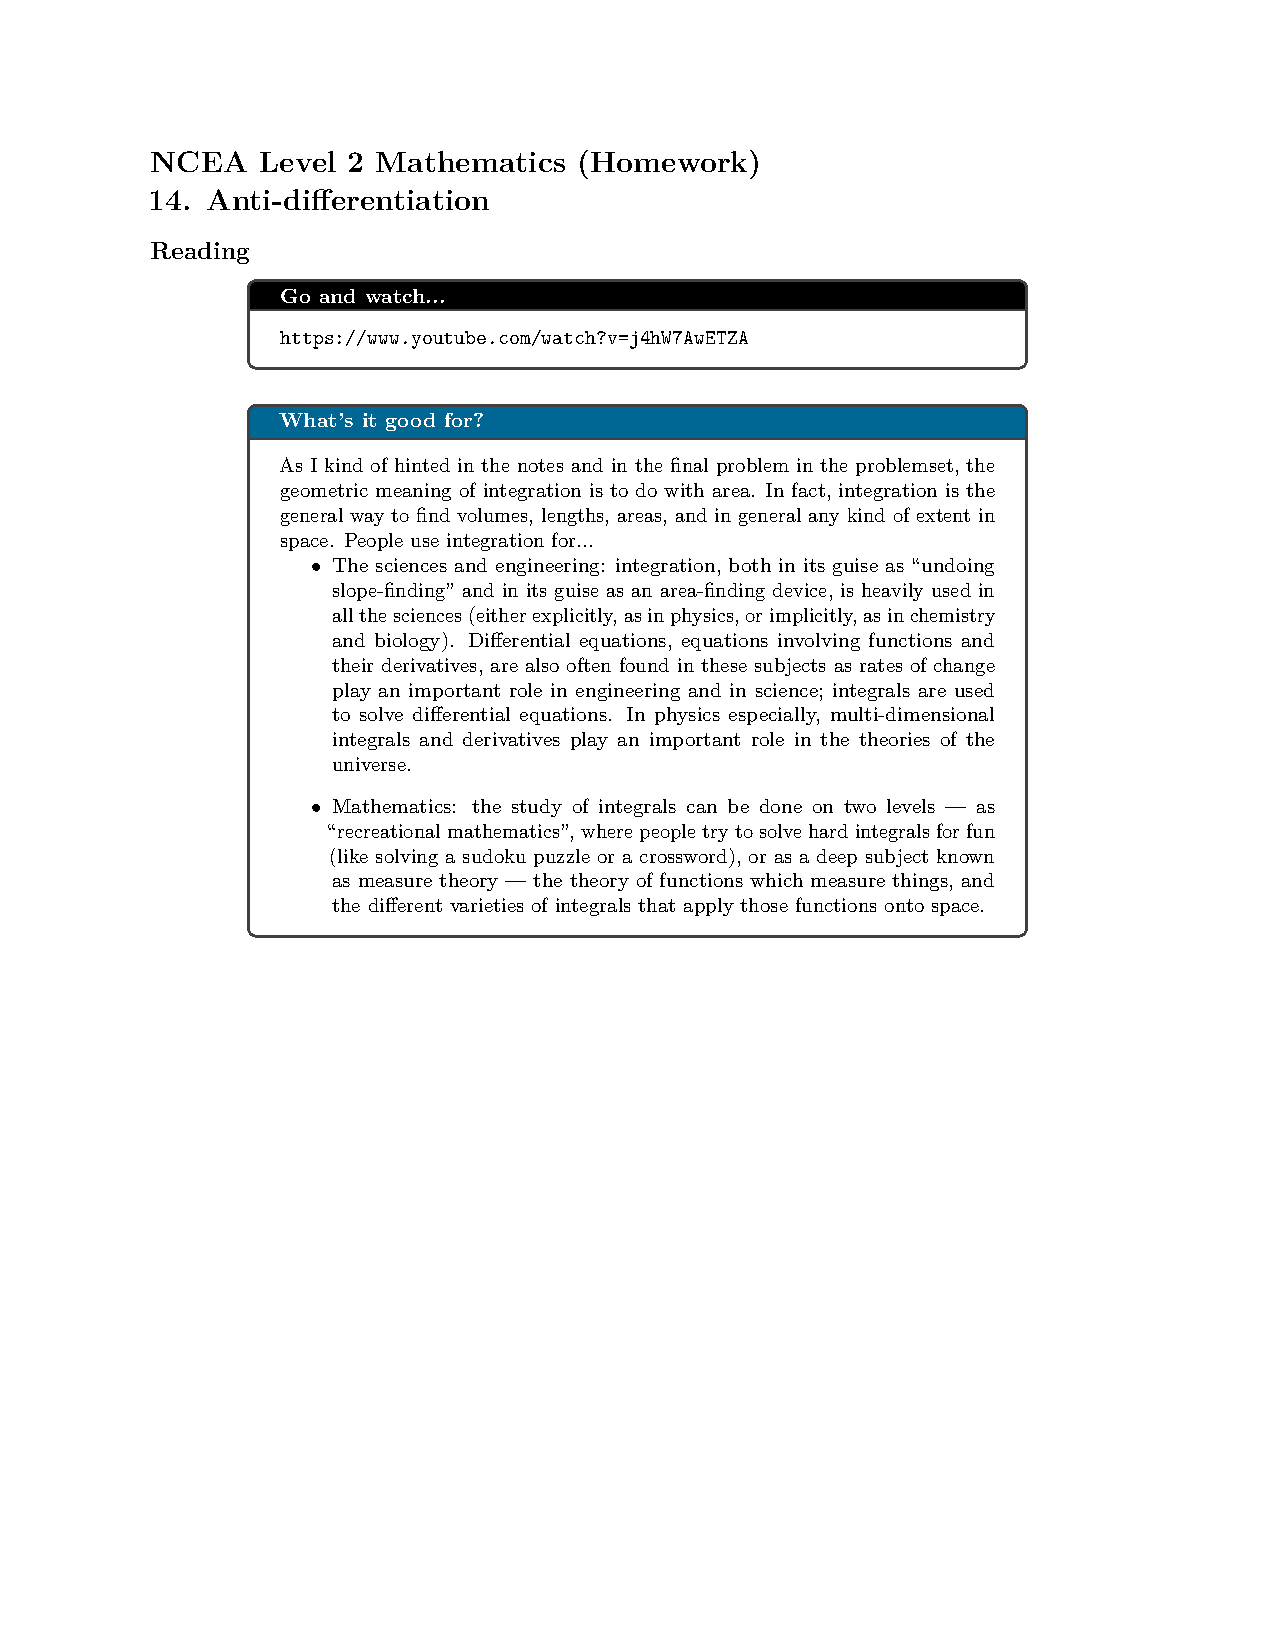
\includepdf[pages={-},pagecommand={}]{14-antidifferentiation-hw.pdf}
  \phantomsection\addcontentsline{toc}{section}{Kinematics and Rates of Change}
  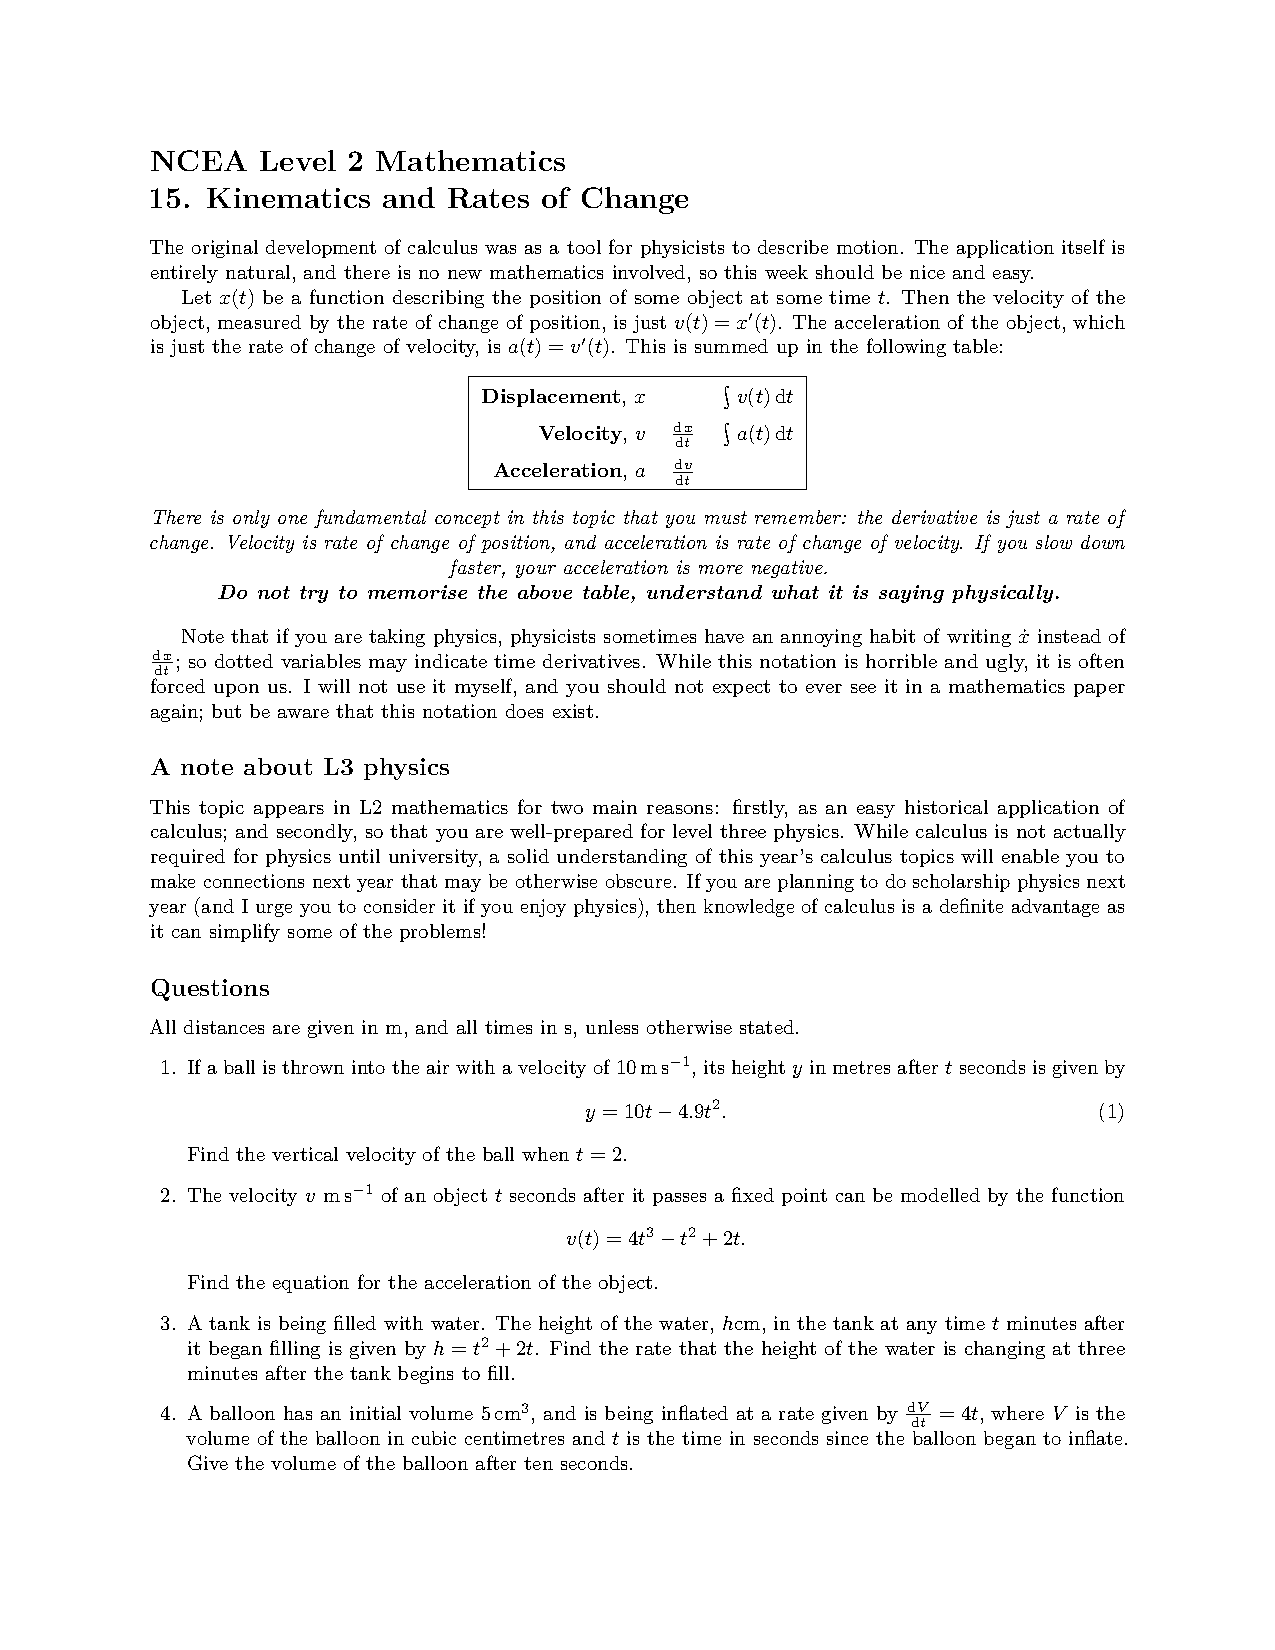
\includepdf[pages={-},pagecommand={}]{15-kinematics.pdf}
  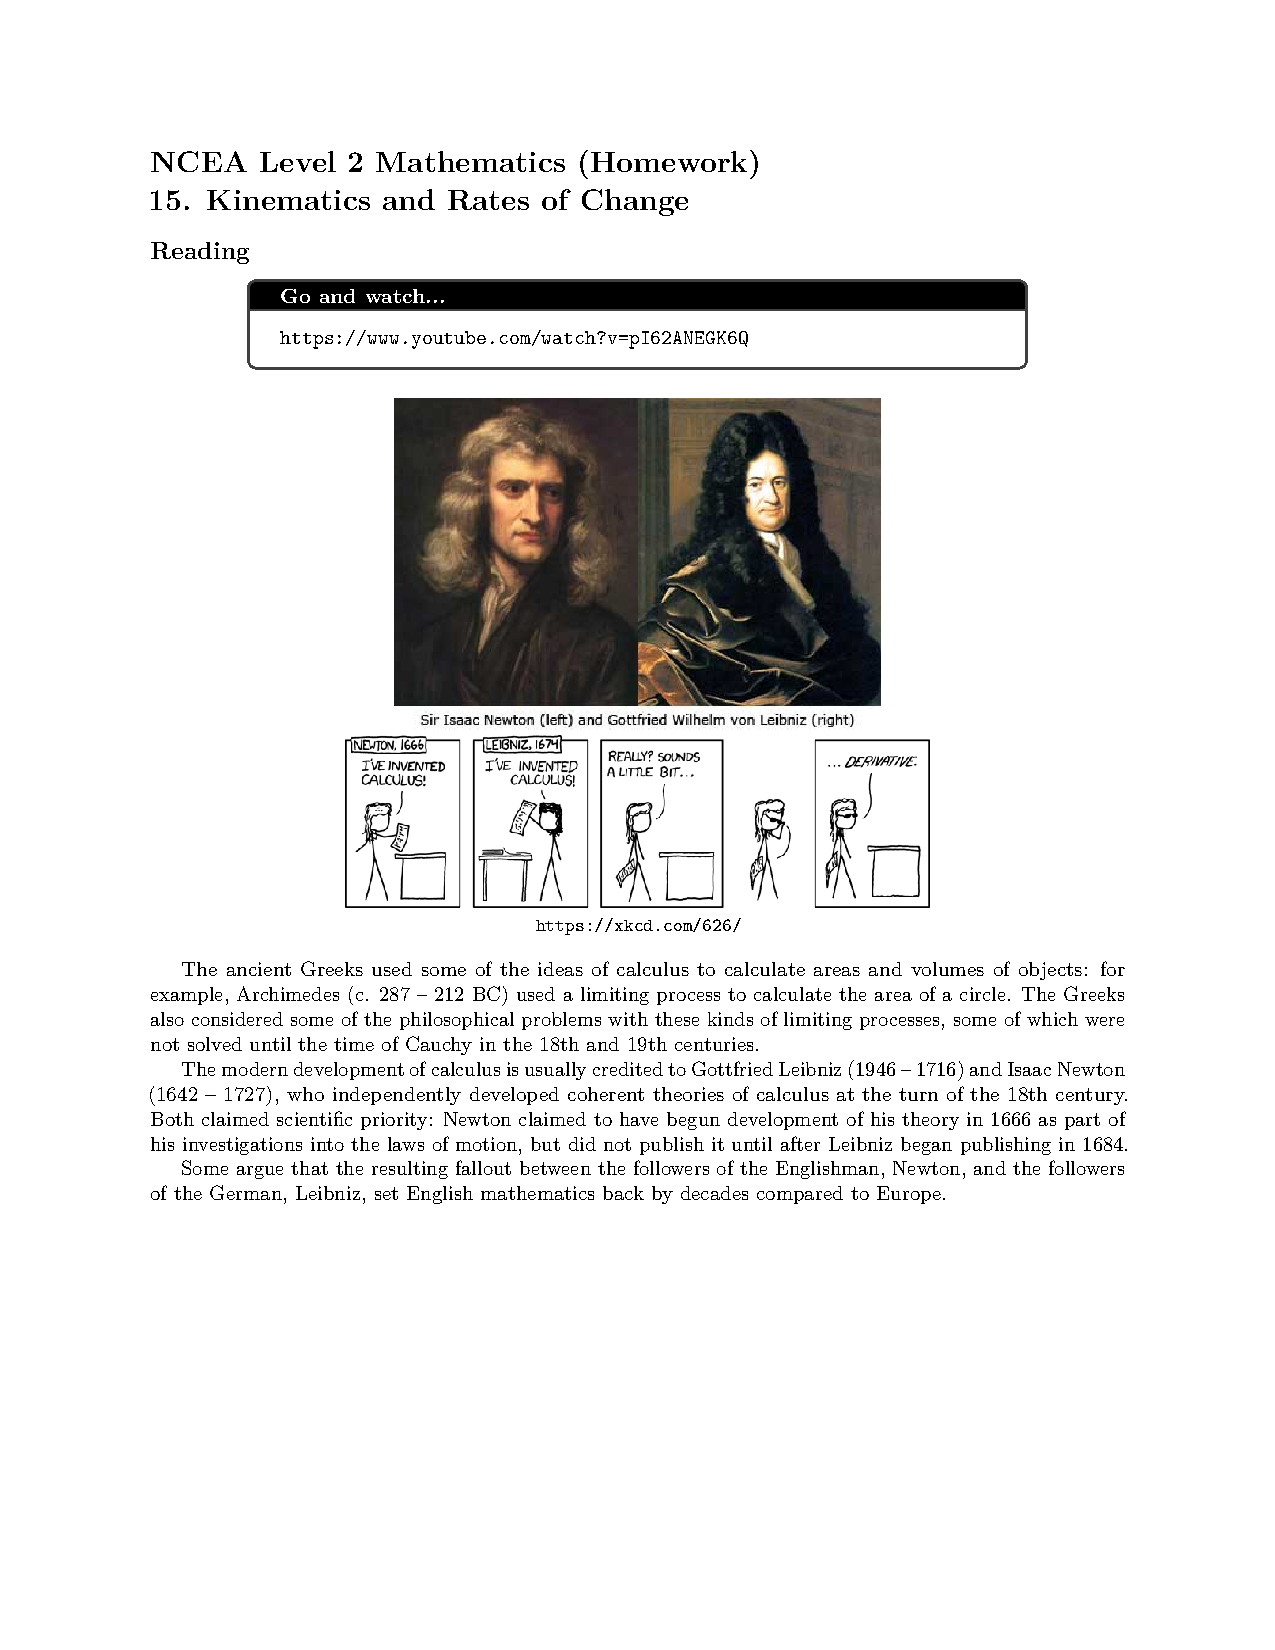
\includepdf[pages={-},pagecommand={}]{15-kinematics-hw.pdf}

  \chapter{Counting}
  \phantomsection\addcontentsline{toc}{section}{Counting and Combinatorics}
  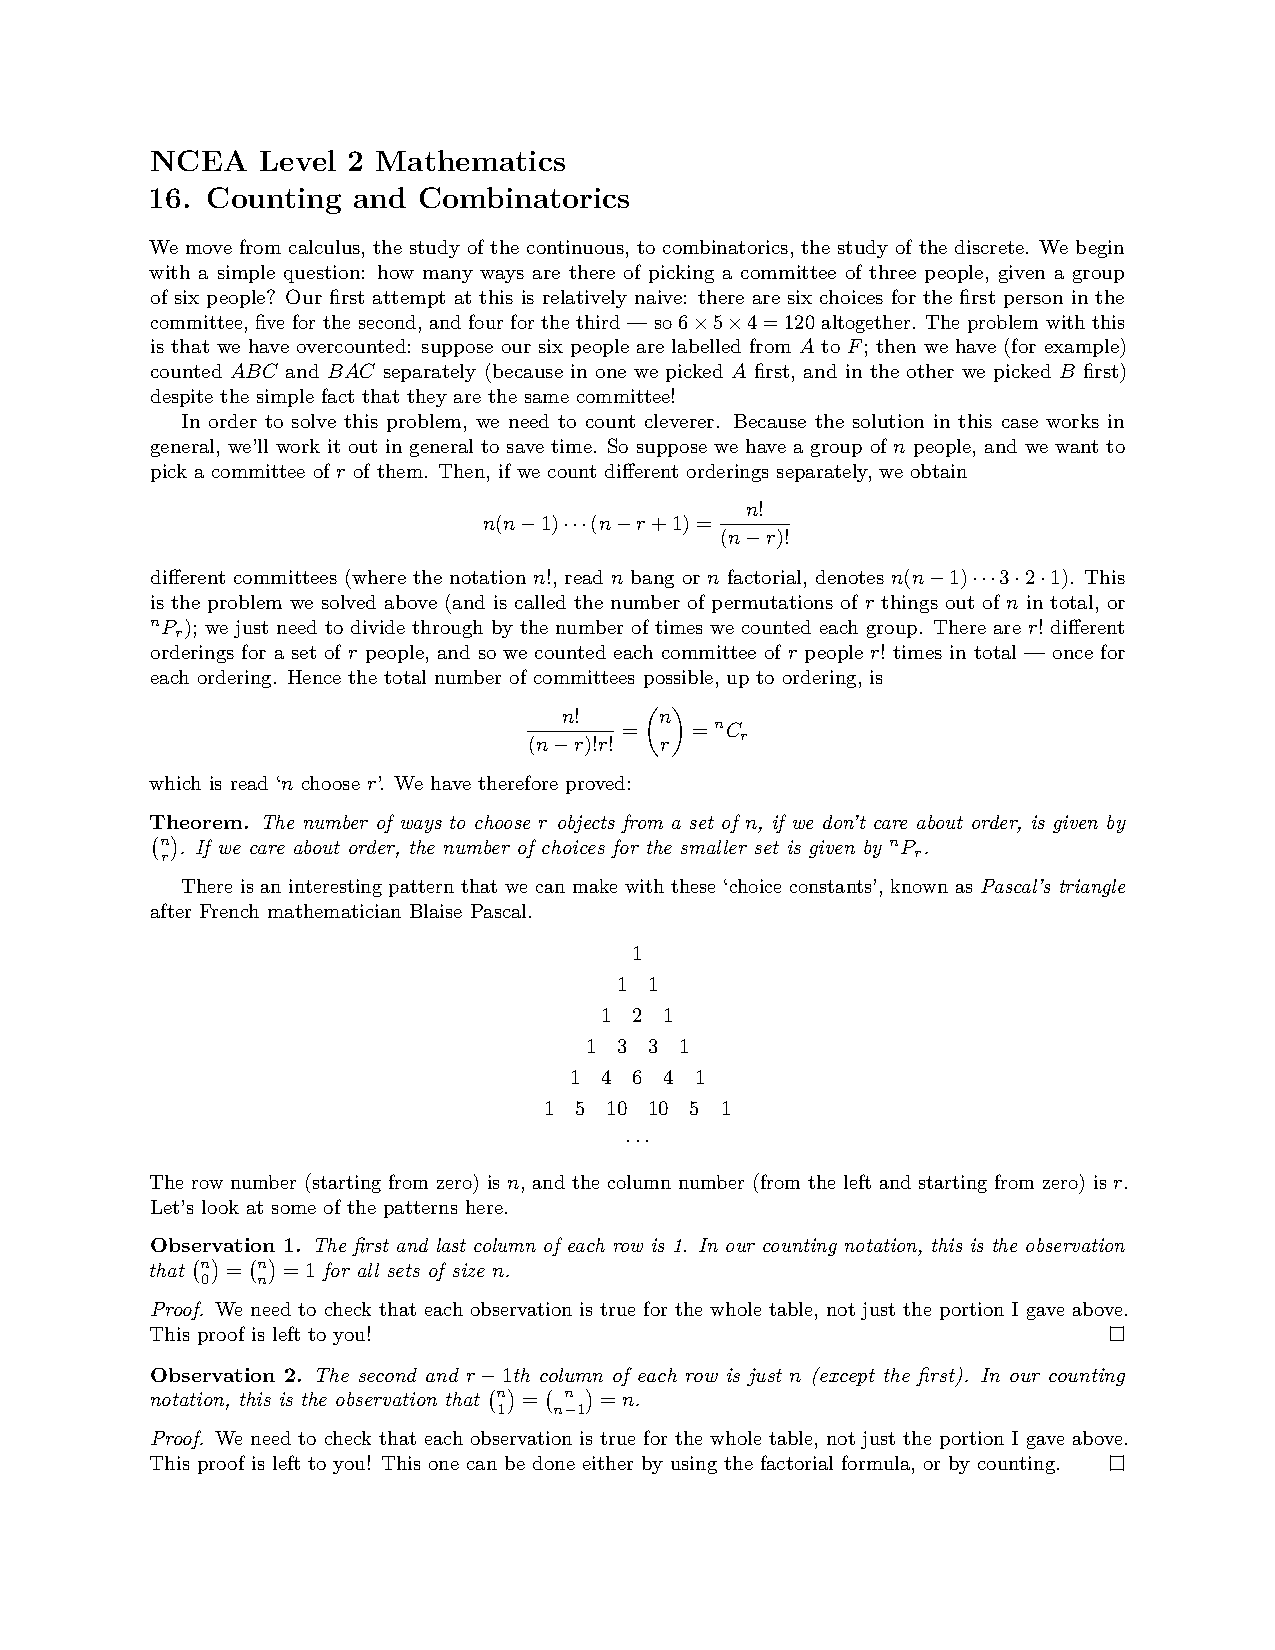
\includepdf[pages={-},pagecommand={}]{16-counting.pdf}
  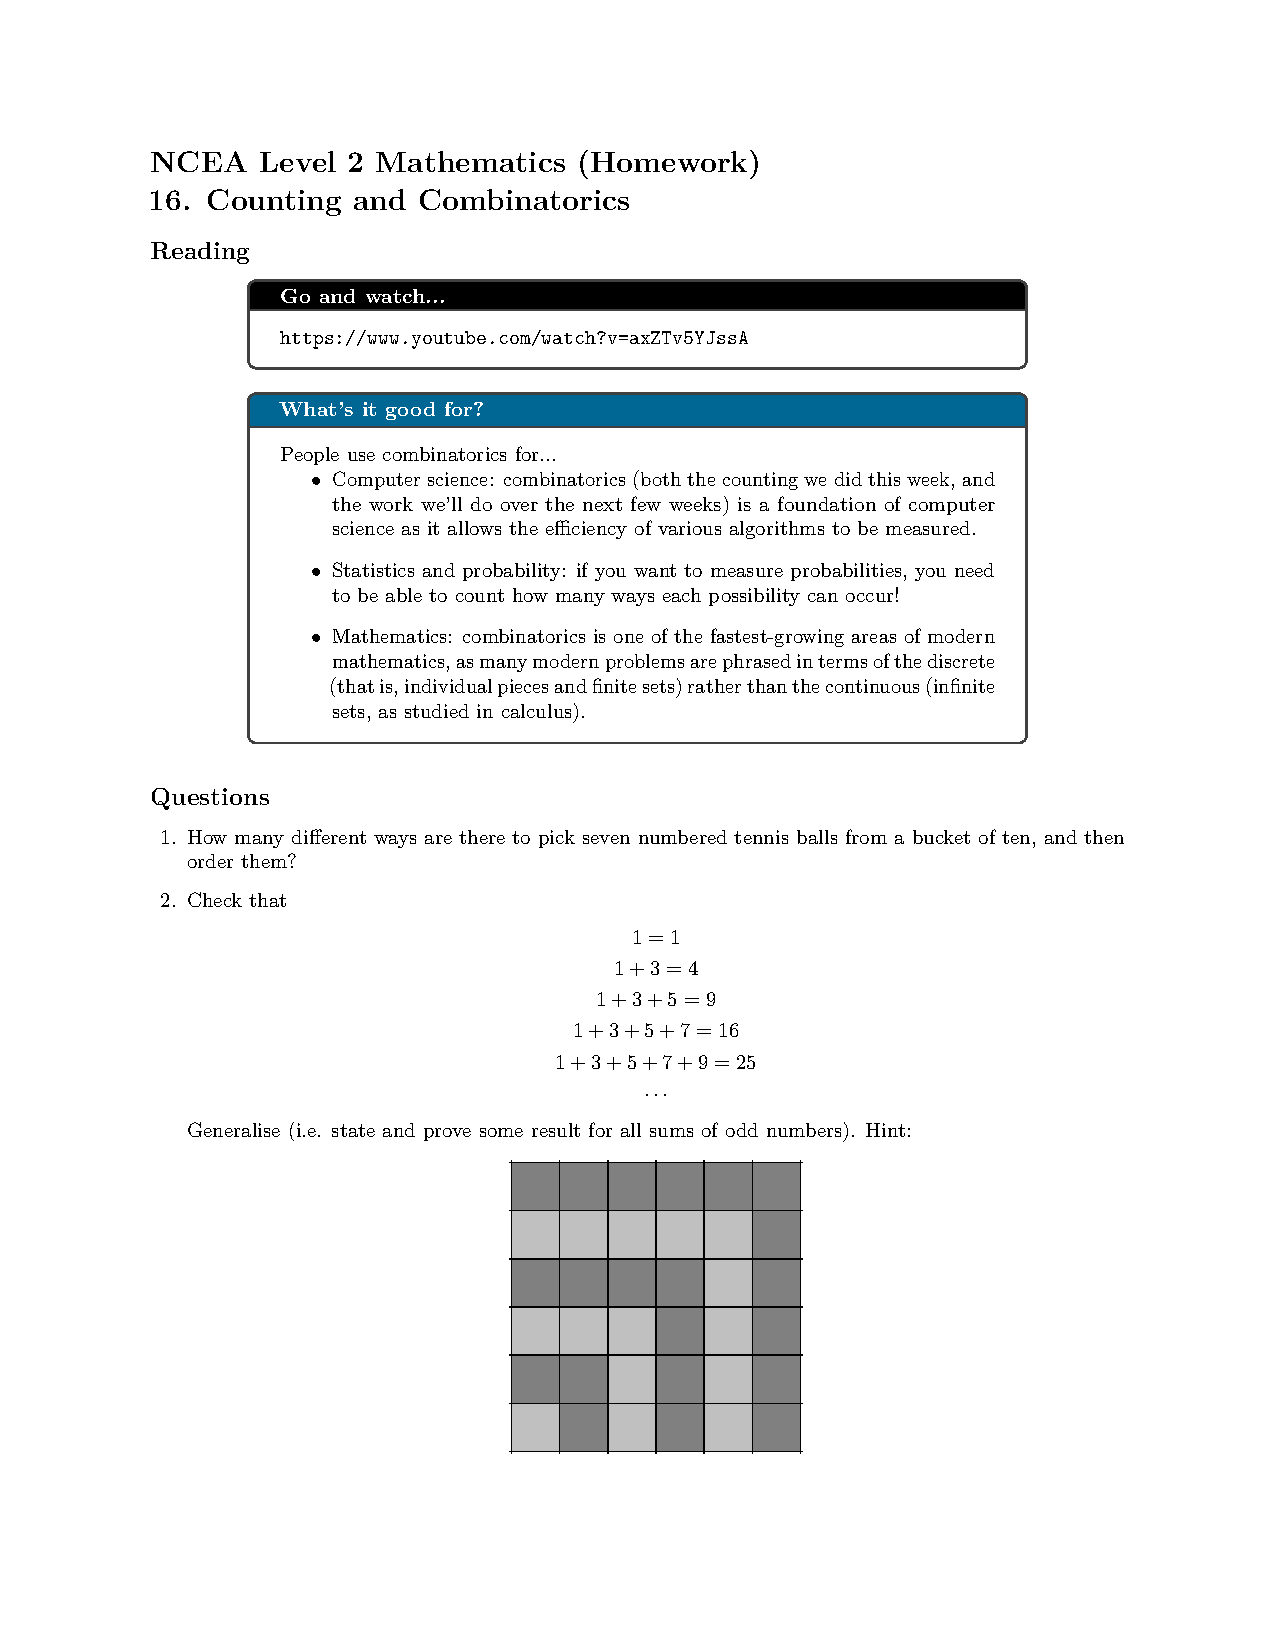
\includepdf[pages={-},pagecommand={}]{16-counting-hw.pdf}
  \phantomsection\addcontentsline{toc}{section}{Number Sequences and Fractals}
  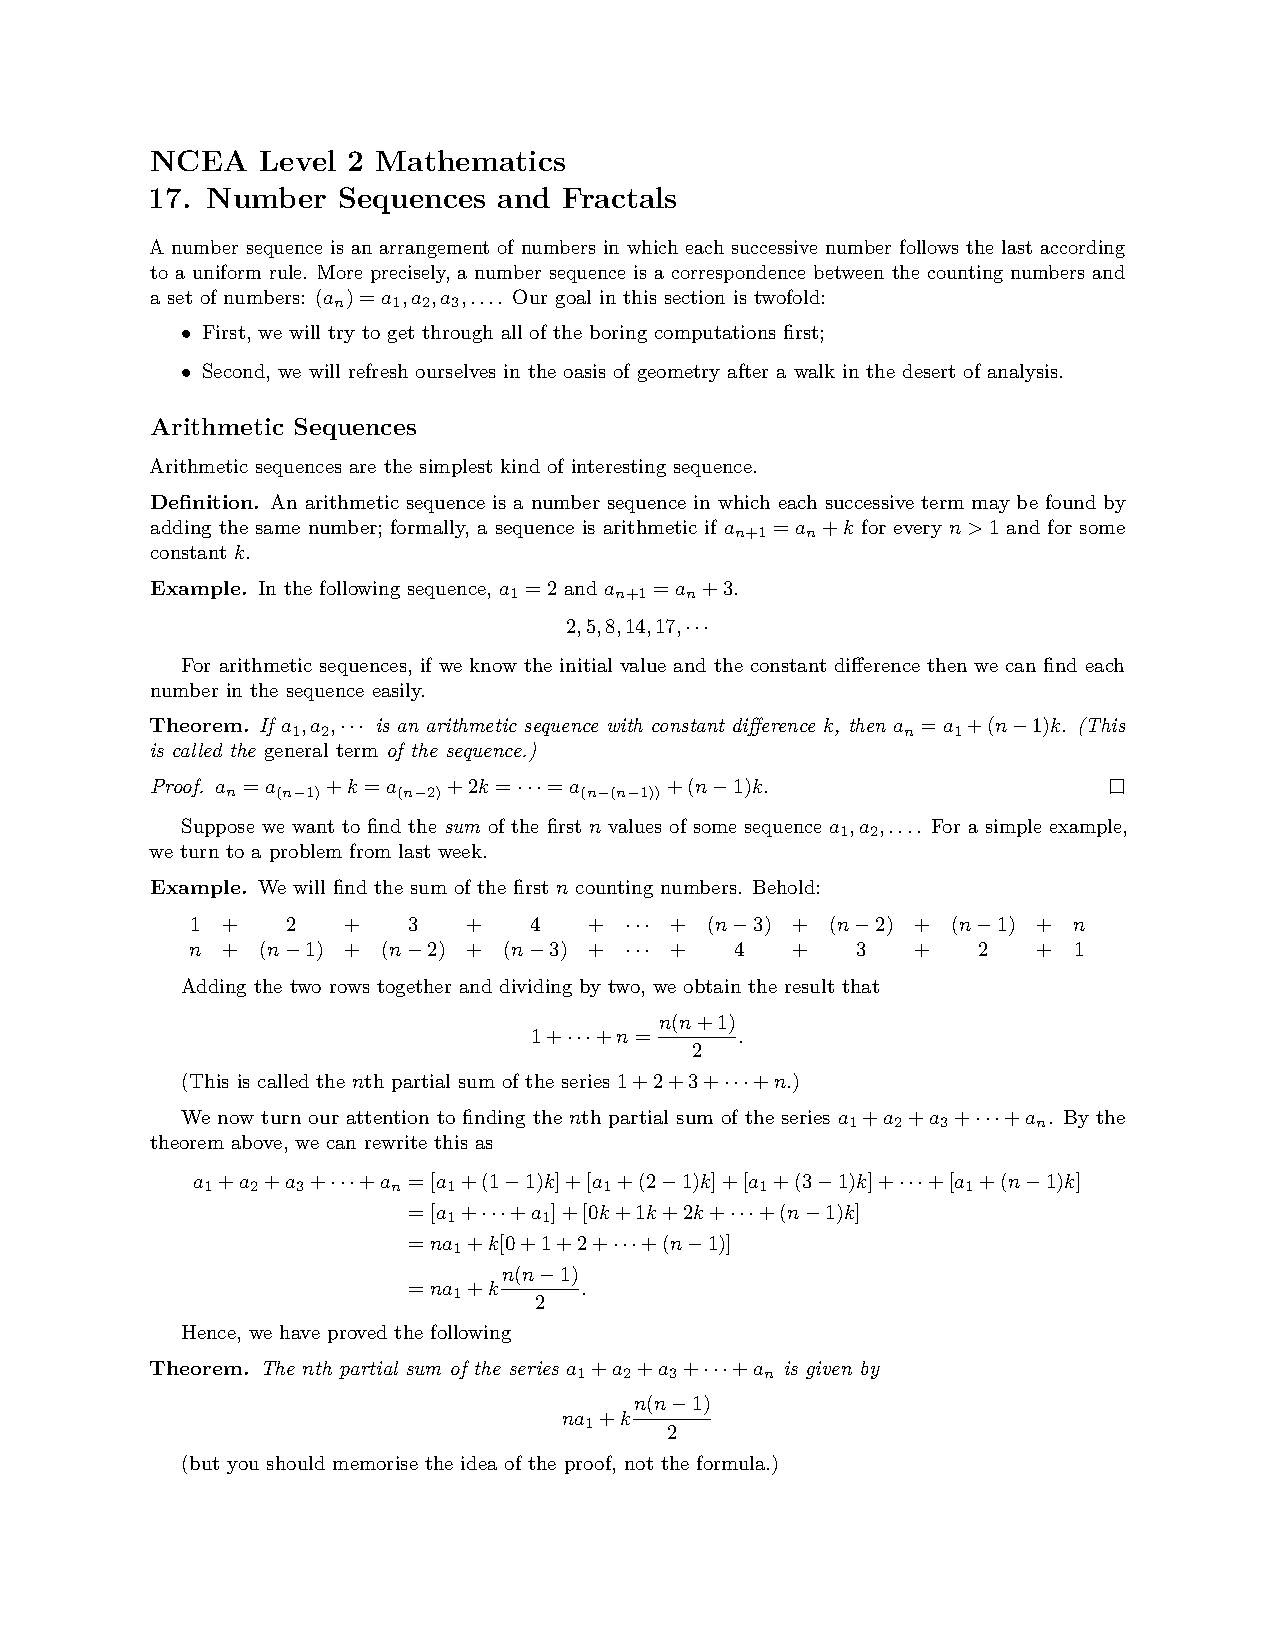
\includepdf[pages={-},pagecommand={}]{17-sequences.pdf}
  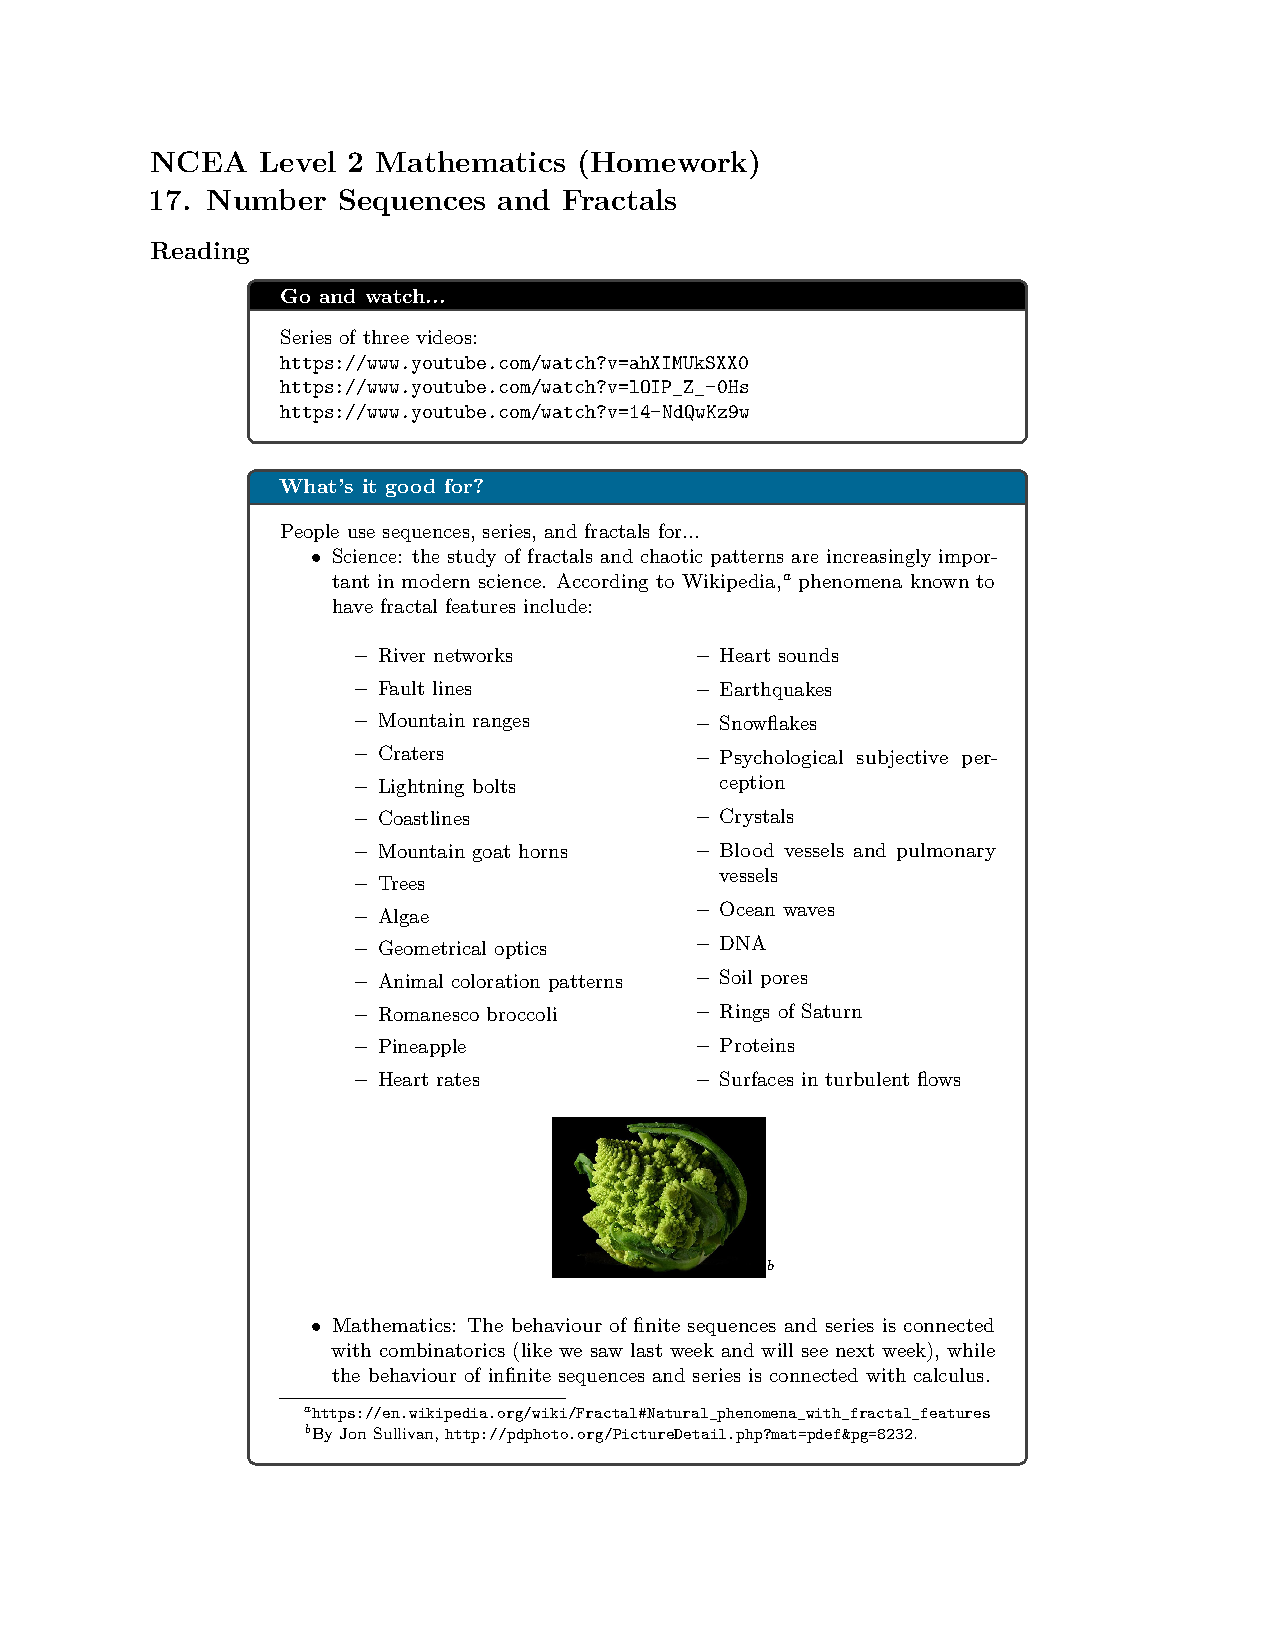
\includepdf[pages={-},pagecommand={}]{17-sequences-hw.pdf}
  \phantomsection\addcontentsline{toc}{section}{Graphs and Networks}
  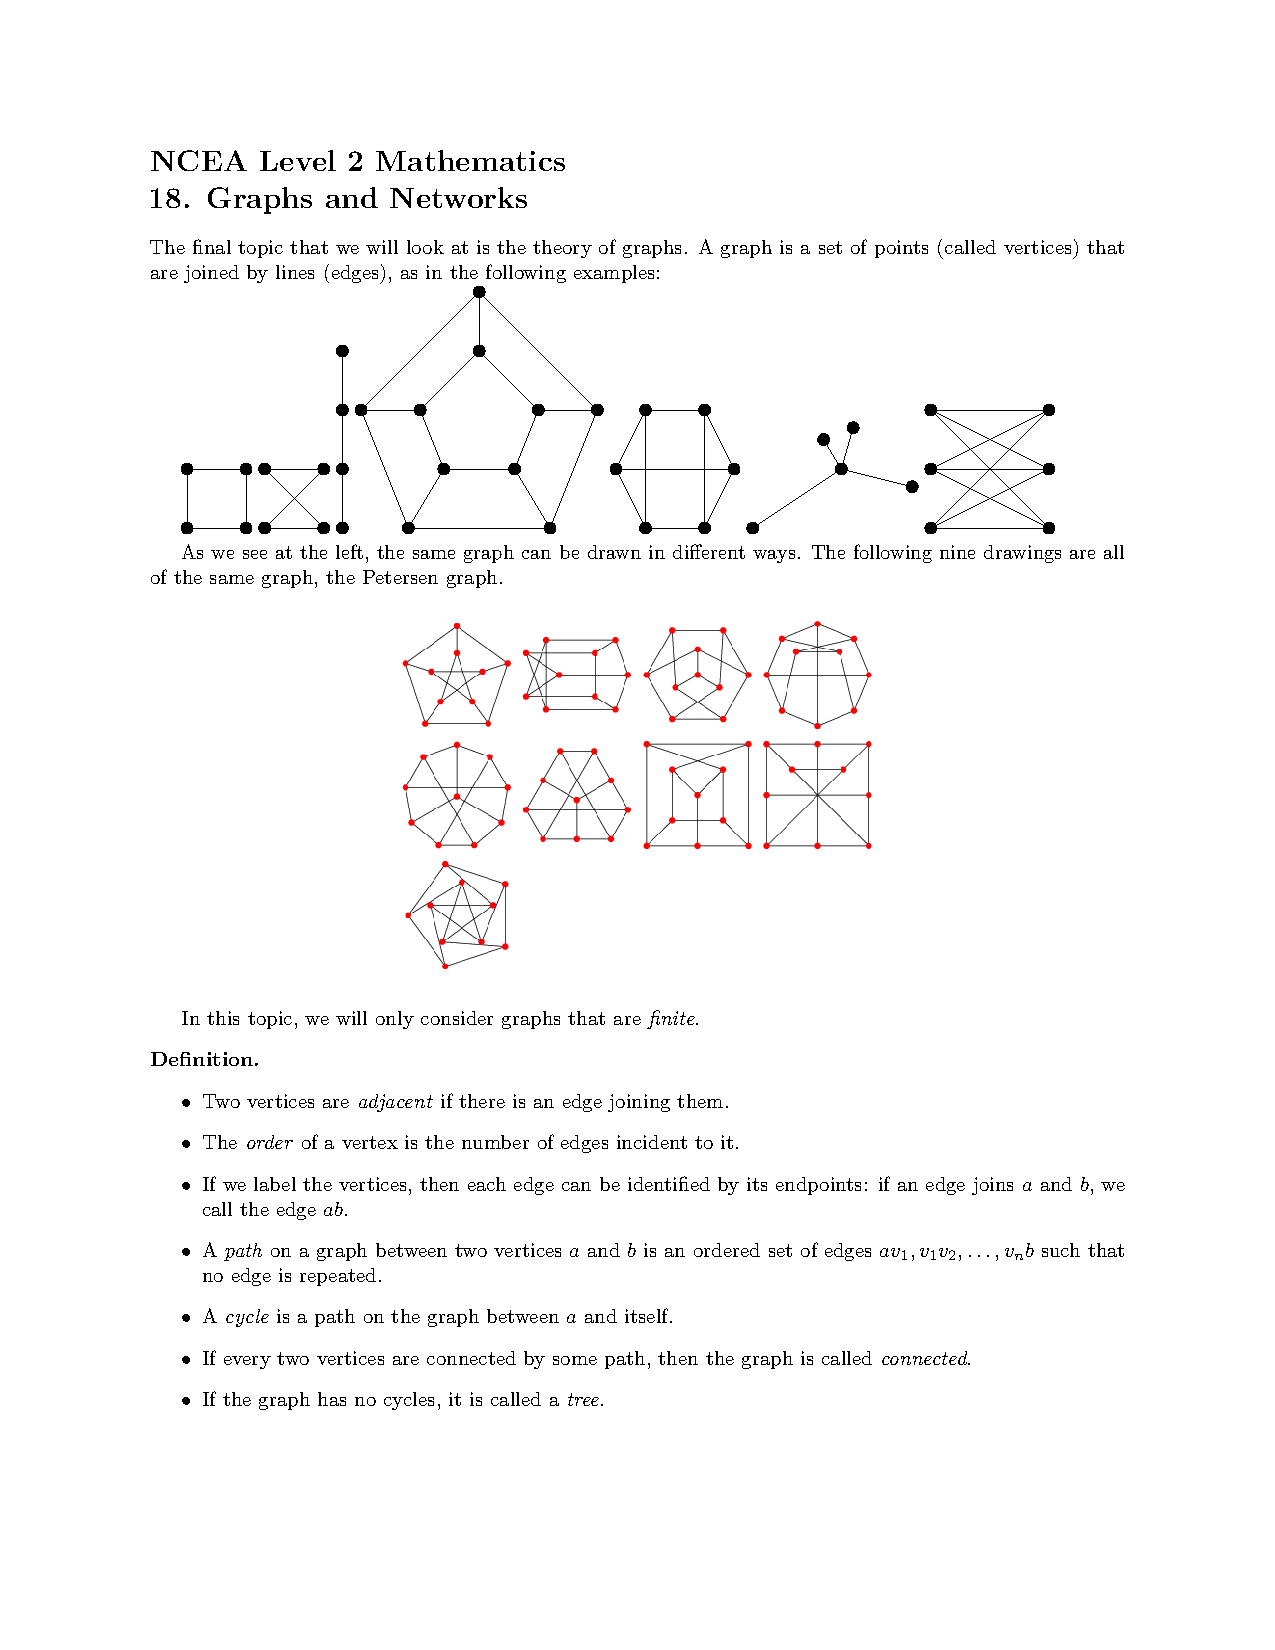
\includepdf[pages={-},pagecommand={}]{18-graphs.pdf}
  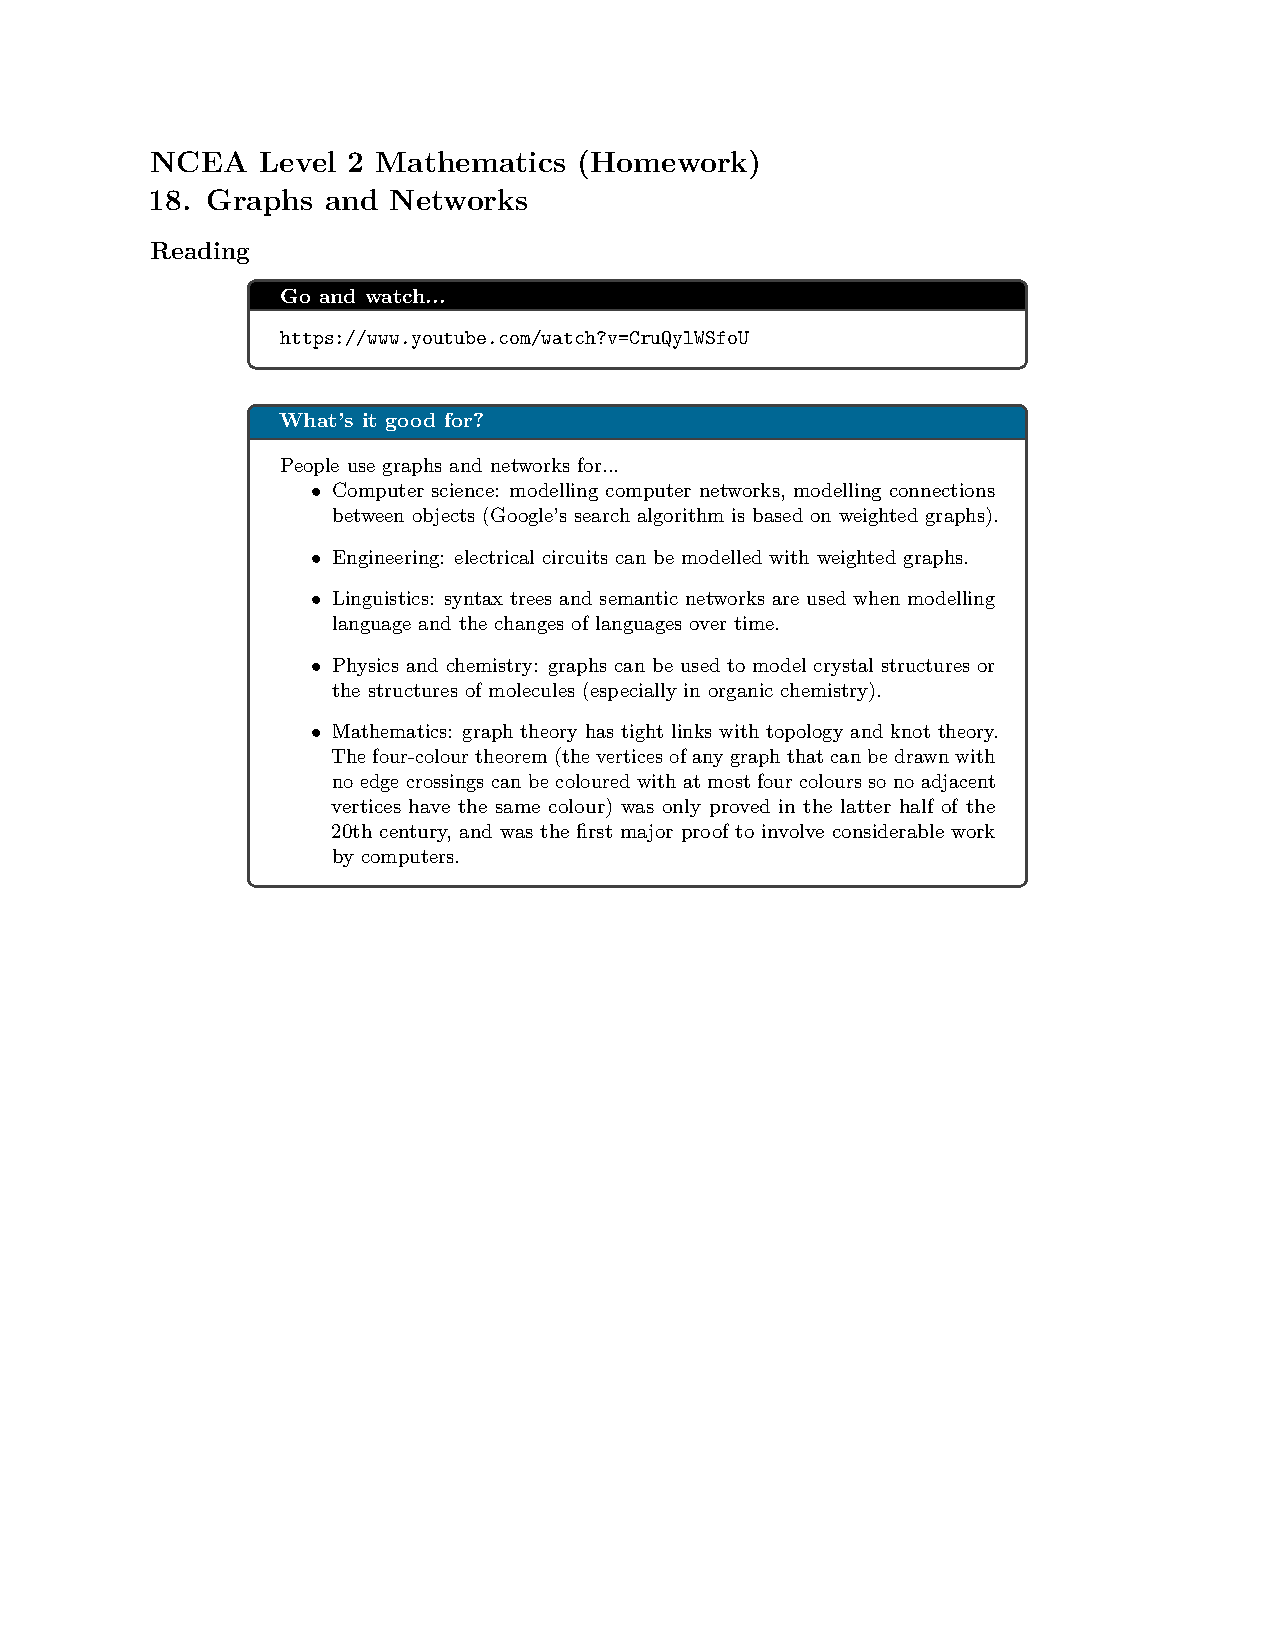
\includepdf[pages={-},pagecommand={}]{18-graphs-hw.pdf}

  \chapter{Statistics}
  \phantomsection\addcontentsline{toc}{section}{The Statistical Enquiry Process}
  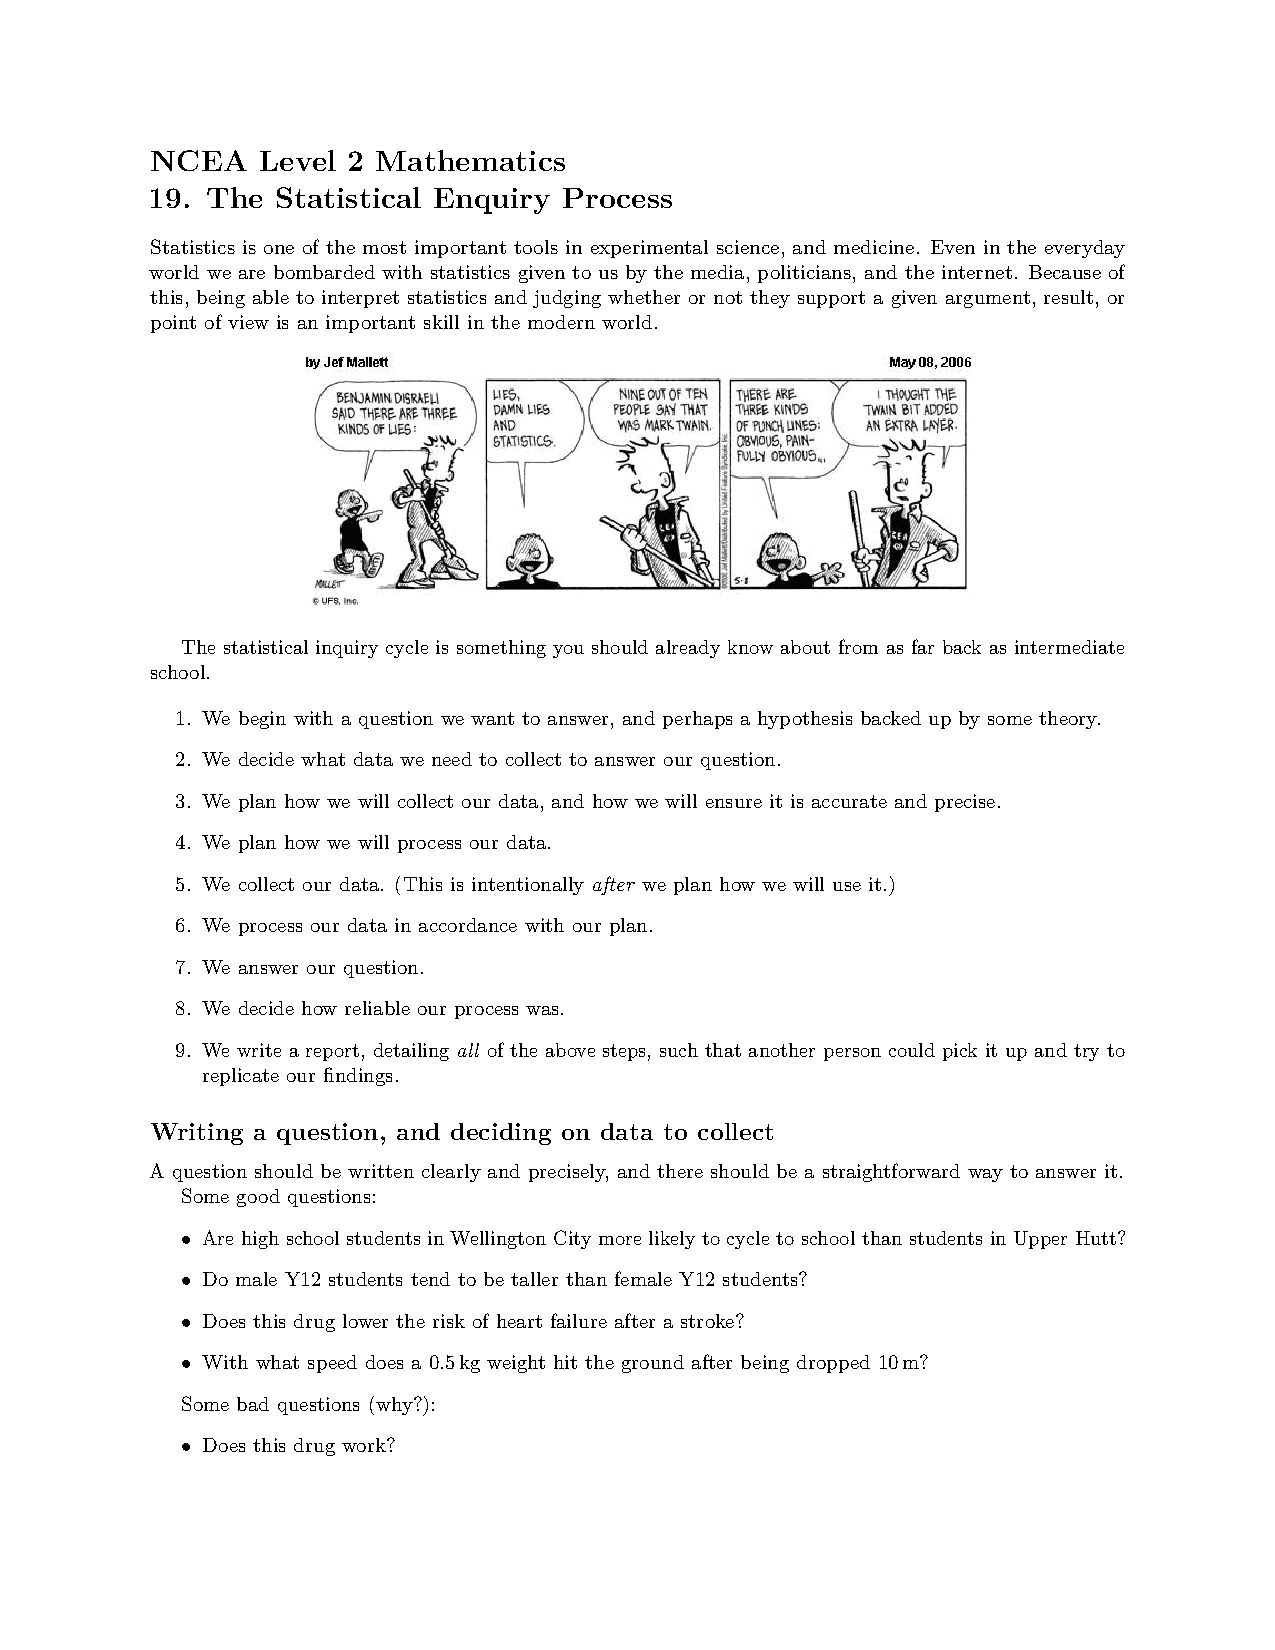
\includepdf[pages={-},pagecommand={}]{19-stats1.pdf}
  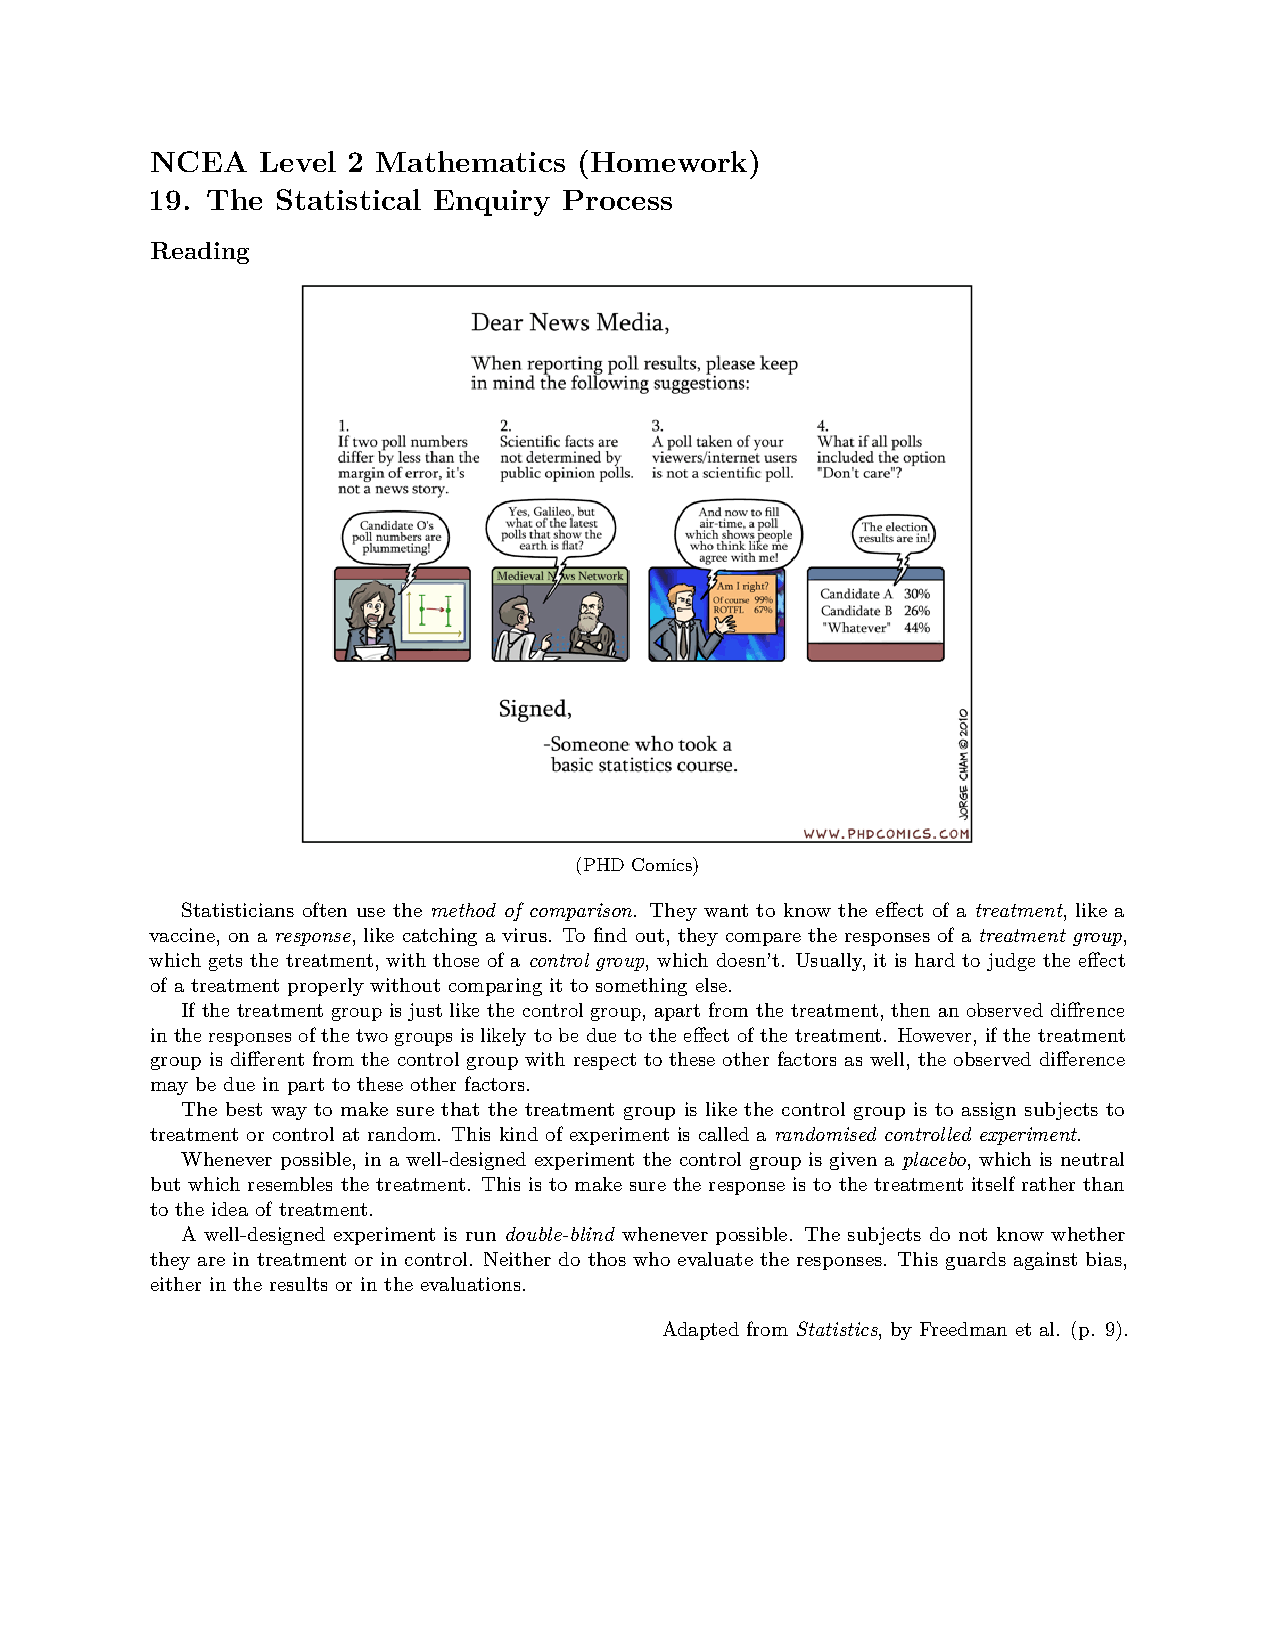
\includepdf[pages={-},pagecommand={}]{19-stats1-hw.pdf}
  \phantomsection\addcontentsline{toc}{section}{Sampling}
  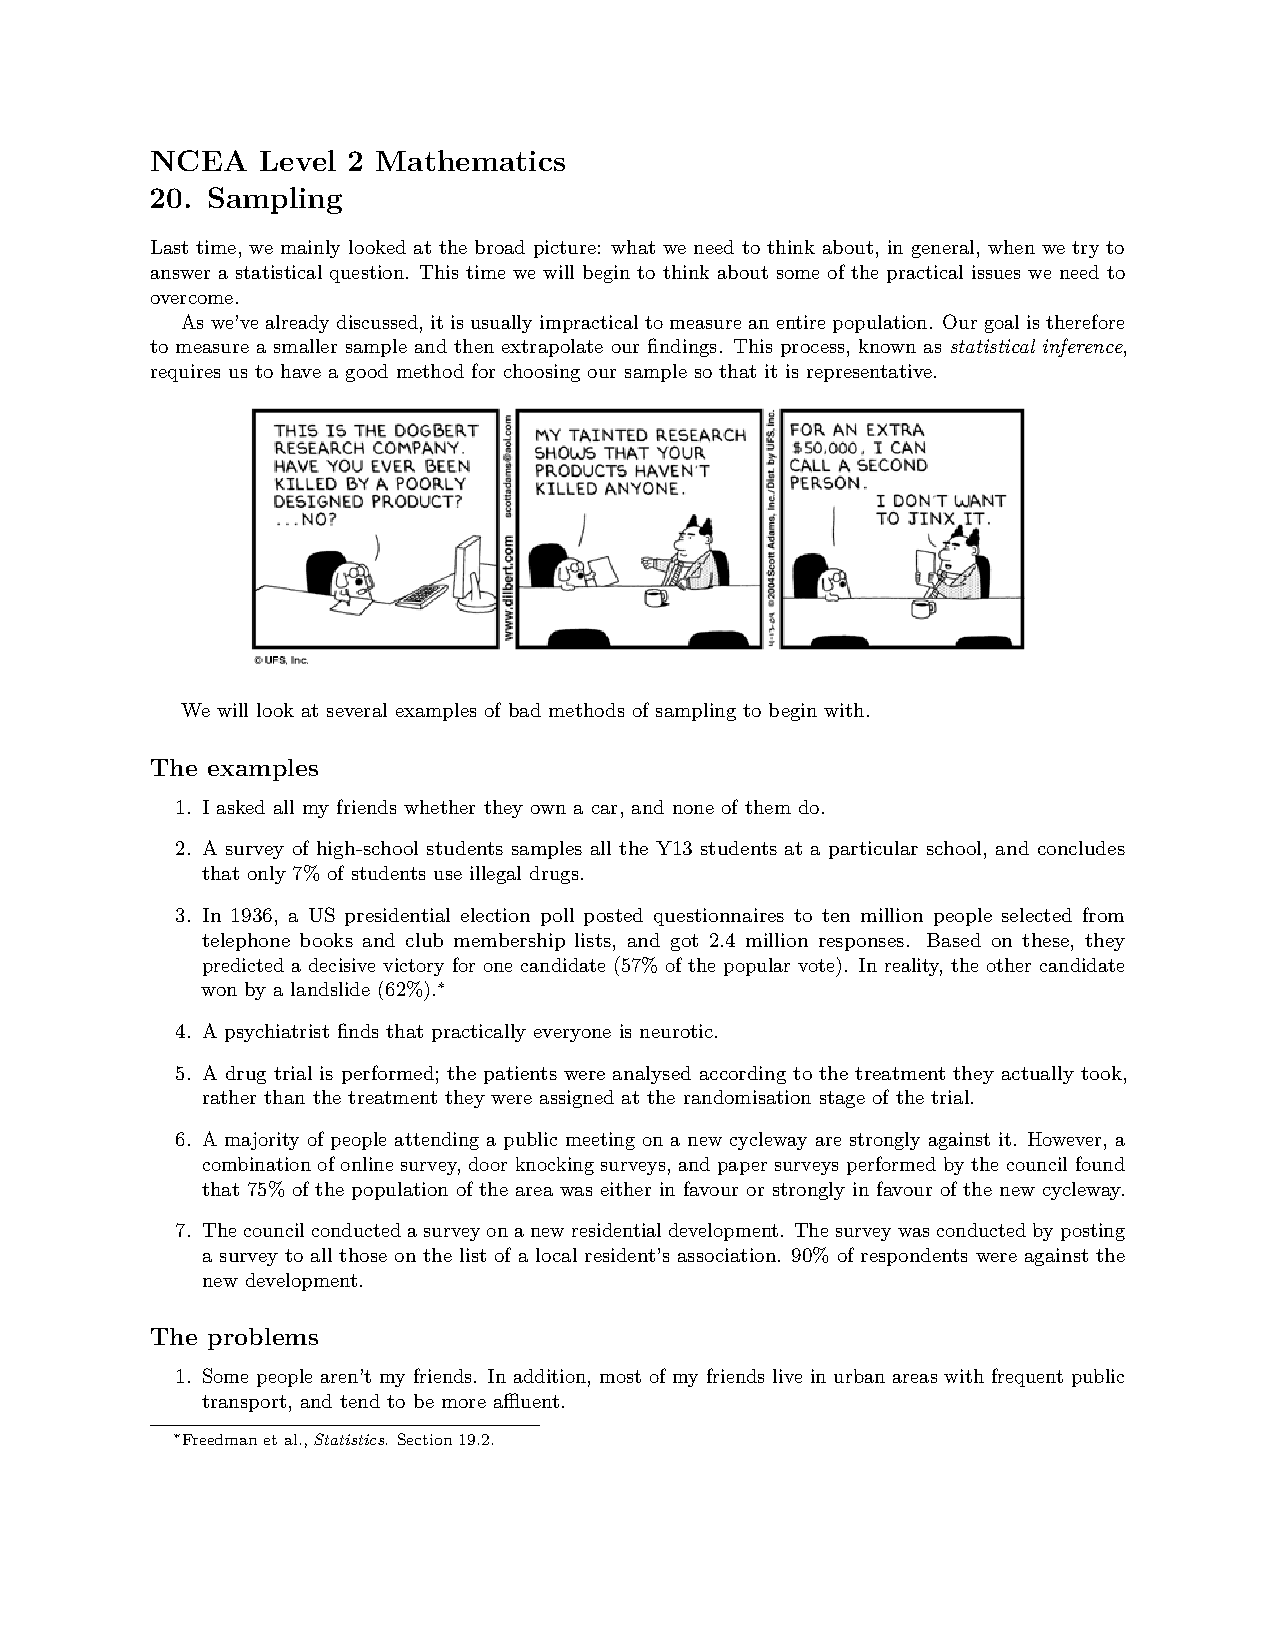
\includepdf[pages={-},pagecommand={}]{20-stats2.pdf}
  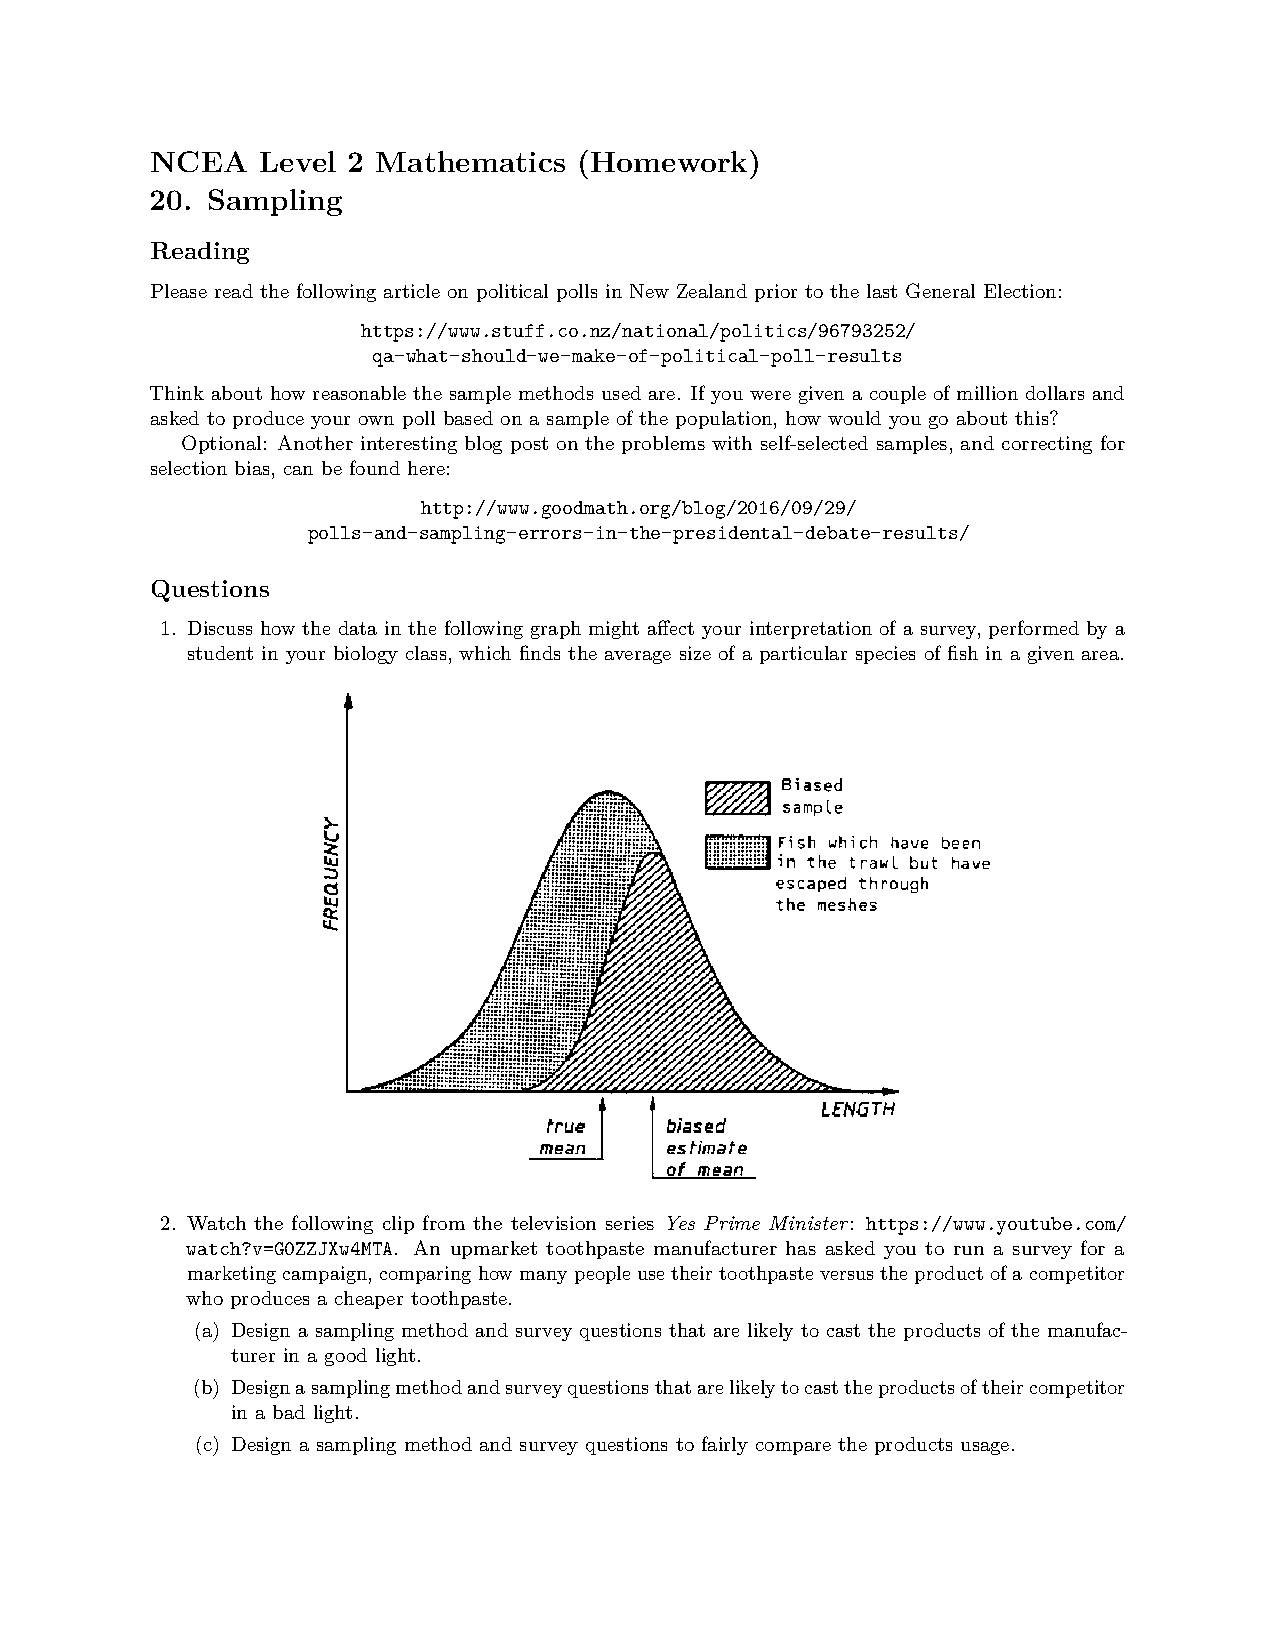
\includepdf[pages={-},pagecommand={}]{20-stats2-hw.pdf}
  \phantomsection\addcontentsline{toc}{section}{Statistical Inference}
  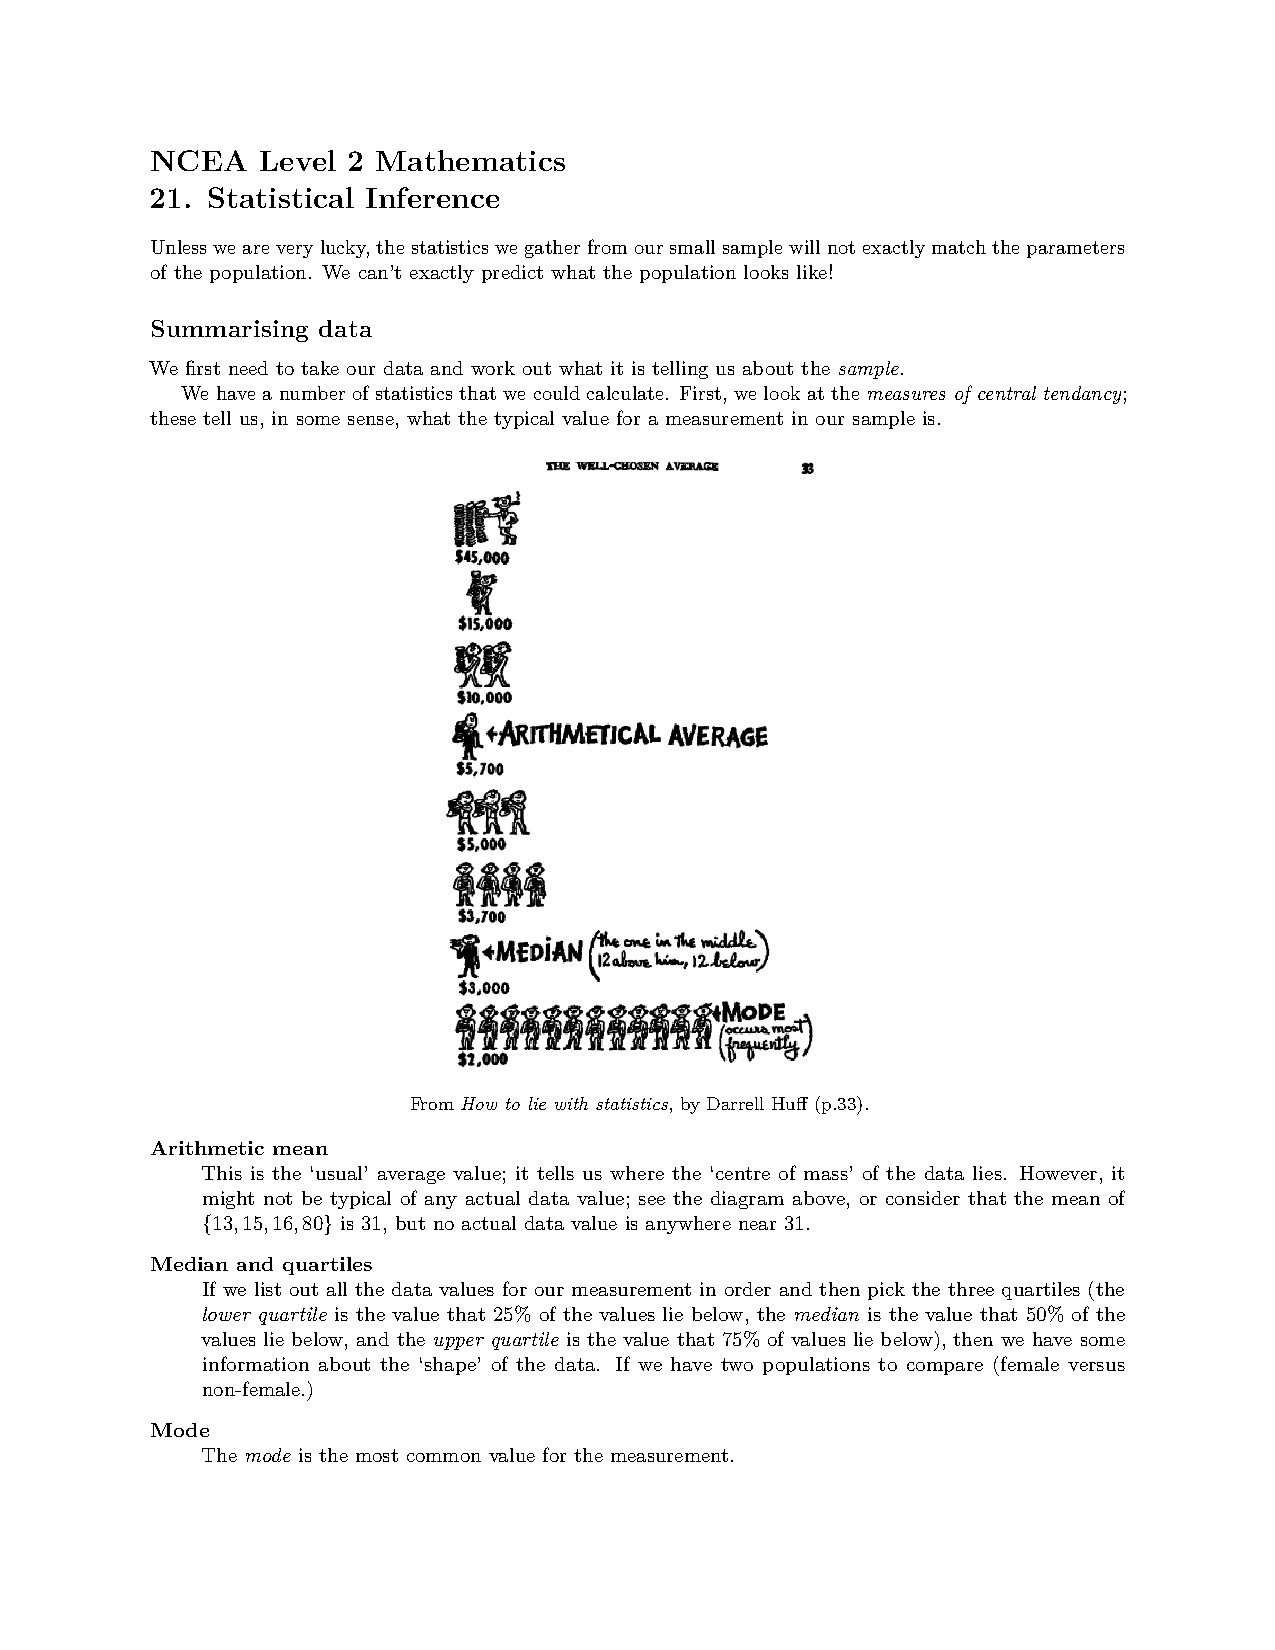
\includepdf[pages={-},pagecommand={}]{21-inference.pdf}
  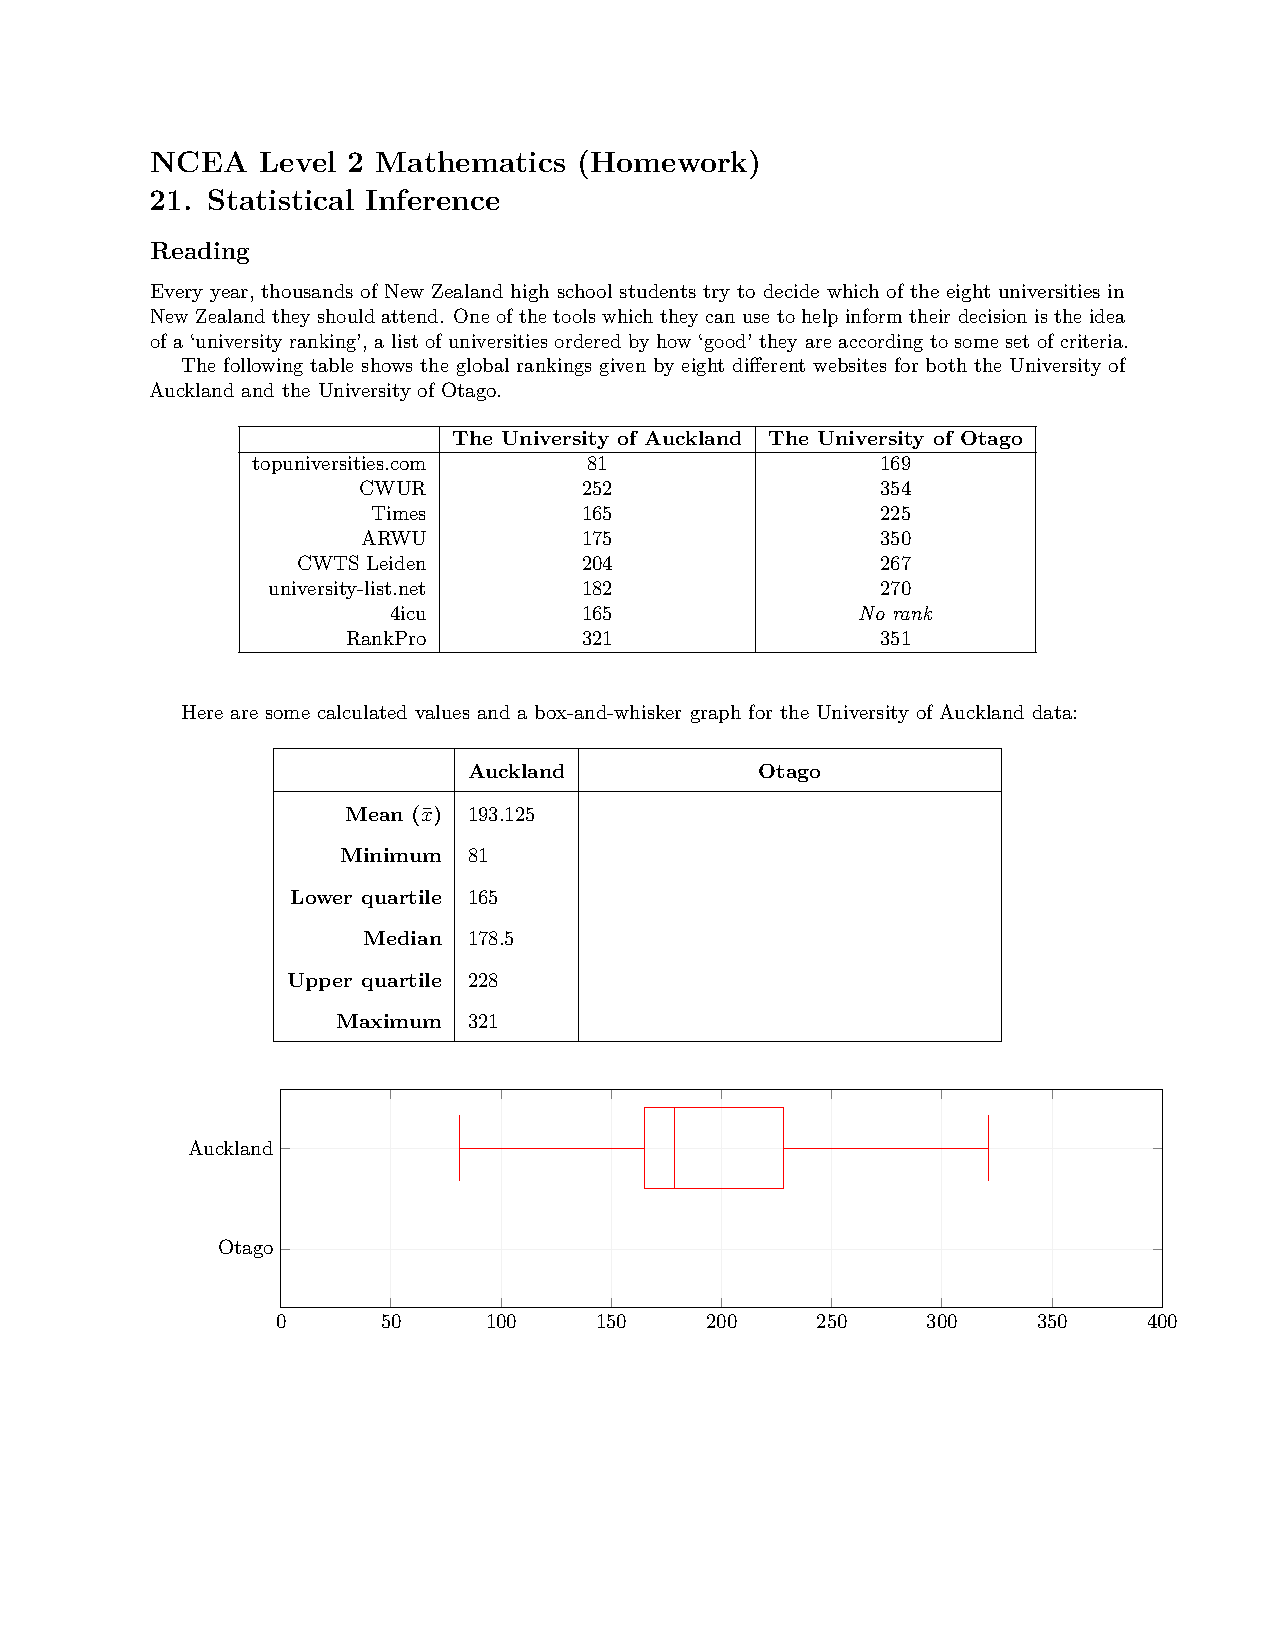
\includepdf[pages={-},pagecommand={}]{21-inference-hw.pdf}
  \phantomsection\addcontentsline{toc}{section}{Probability and Risk}
  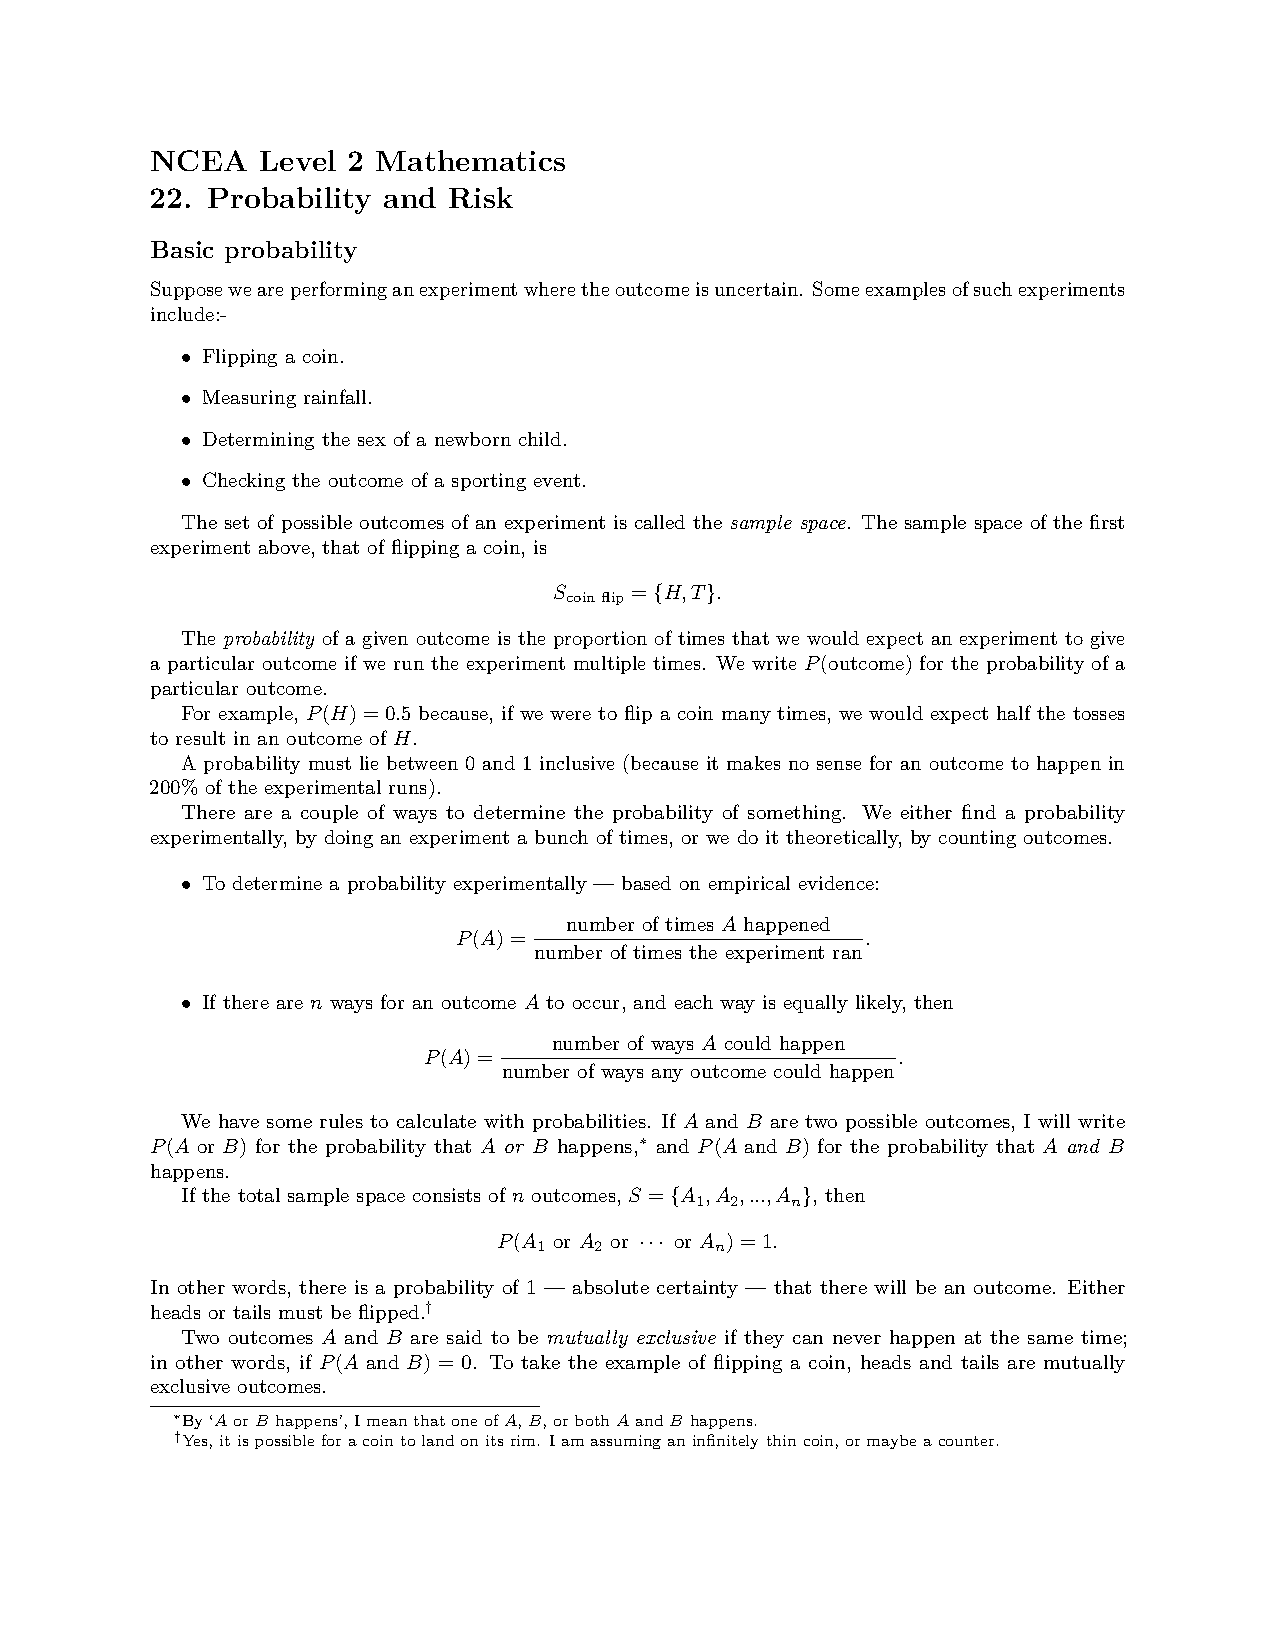
\includepdf[pages={-},pagecommand={}]{22-prob1.pdf}
  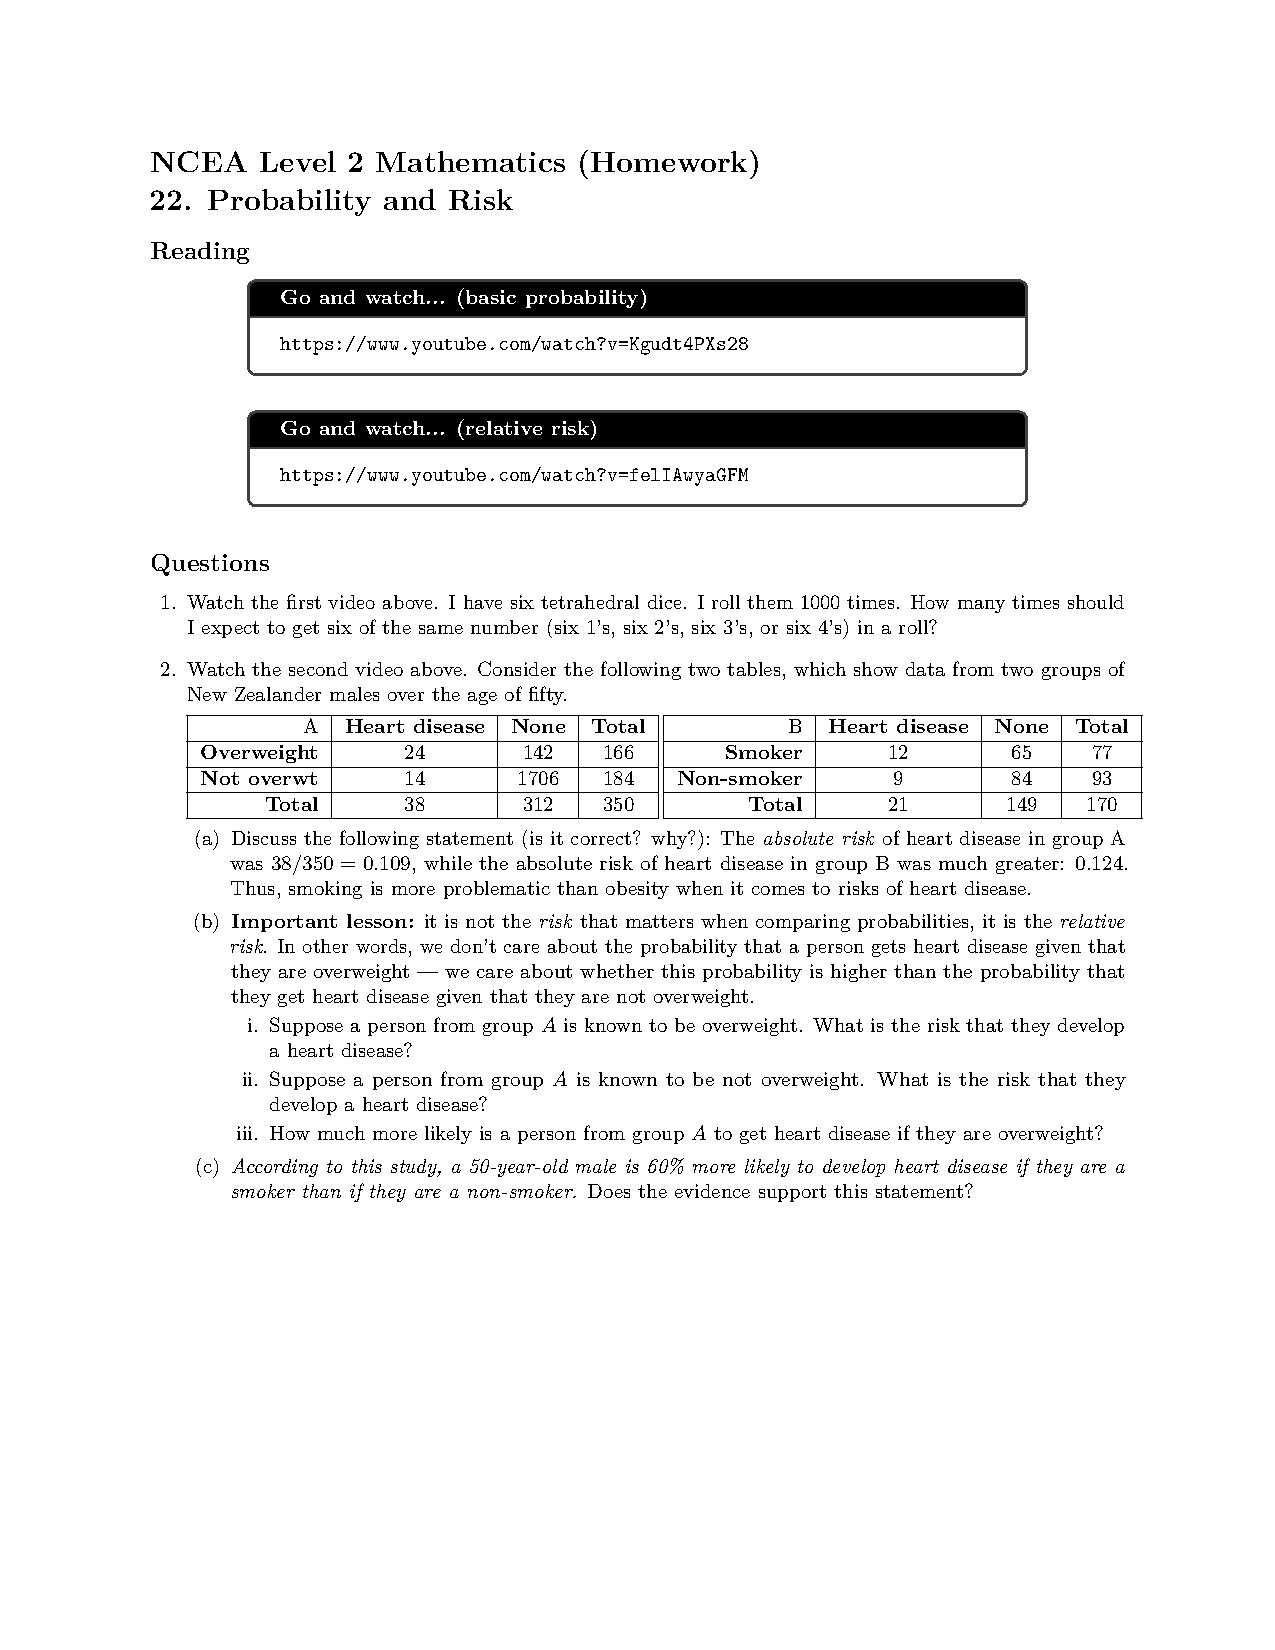
\includepdf[pages={-},pagecommand={}]{22-prob1-hw.pdf}
  \phantomsection\addcontentsline{toc}{section}{Probability Distributions}
  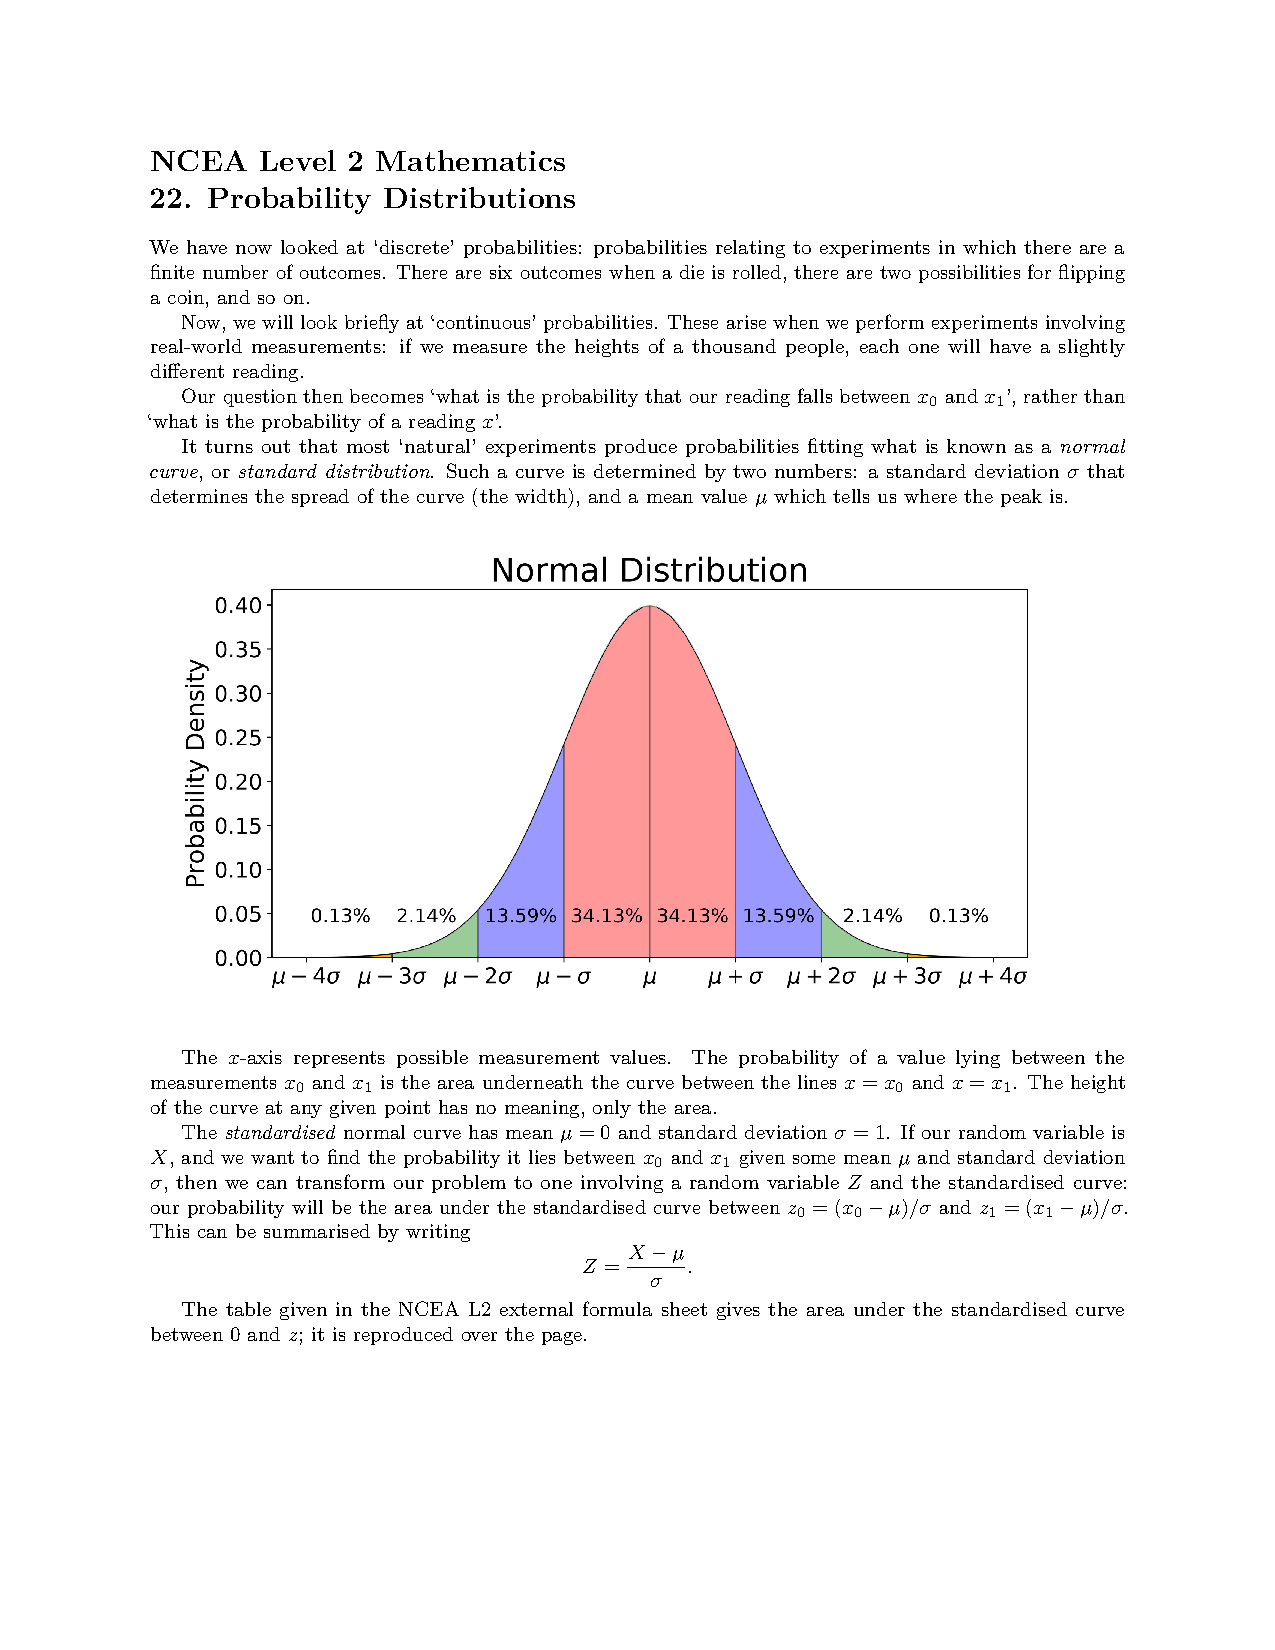
\includepdf[pages={-},pagecommand={}]{23-prob2.pdf}
  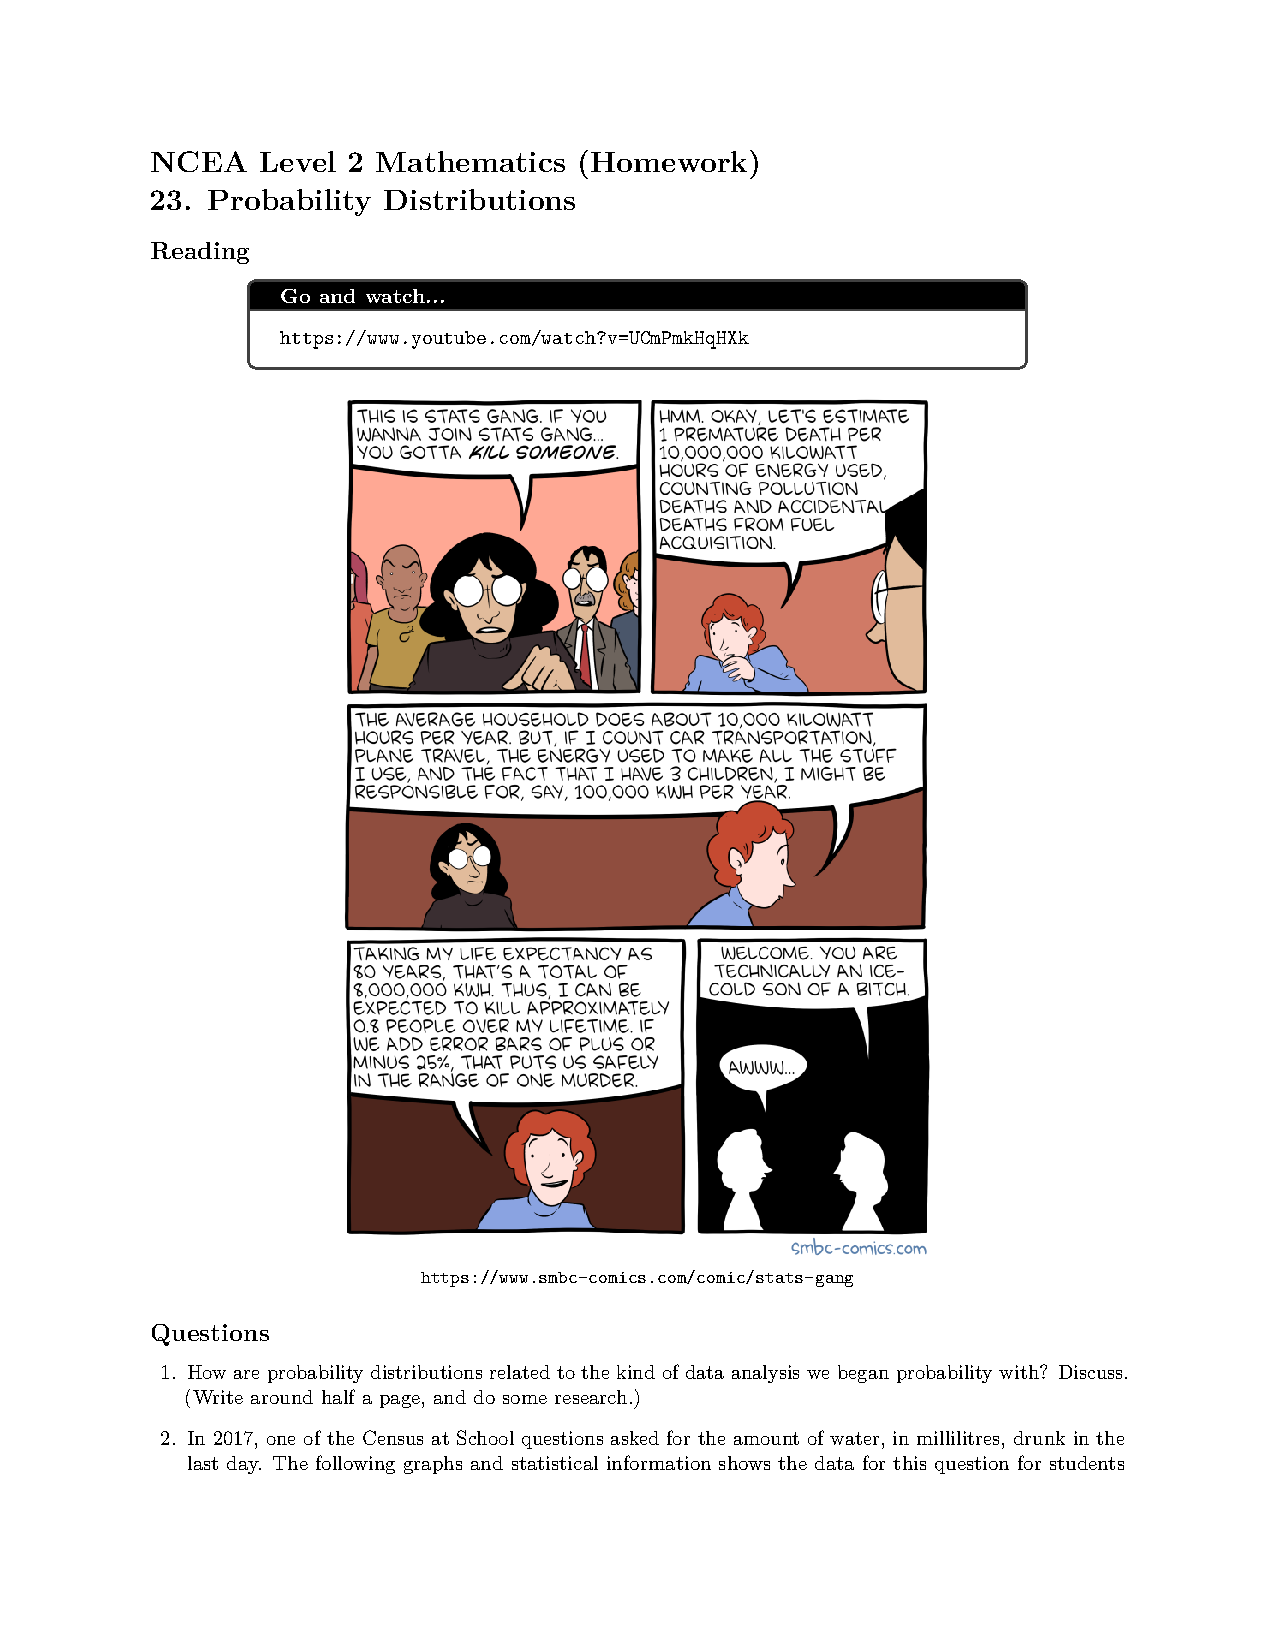
\includepdf[pages={-},pagecommand={}]{23-prob2-hw.pdf}

  \chapter{Addendum}
  \phantomsection\addcontentsline{toc}{section}{Bibliography and Further Reading}
  \includepdf[pages={-},pagecommand={}]{99-bibliography.pdf}

\end{document}
